% document set up
\documentclass{article}
\usepackage[utf8]{inputenc}
\usepackage{fullpage}
\setlength{\parindent}{0cm}
\setlength{\parskip}{1em}

% math packages
\usepackage{amsfonts}
\usepackage{amsmath}
\usepackage{amssymb}
\usepackage{amsthm}
\usepackage{enumitem}
\usepackage{bbm}
\setlist[itemize]{leftmargin=*}

% general packages
\usepackage[colorlinks=true,linkcolor=blue,citecolor=blue]{hyperref}
\usepackage{natbib}

% algorithms
\usepackage[ruled,vlined]{algorithm2e}
\newcommand\mycommfont[1]{\footnotesize\ttfamily\textcolor{blue}{#1}}
\SetCommentSty{mycommfont}


% plate diagram
\usepackage{tikz}
\usetikzlibrary{bayesnet}

\newcommand\indep{\perp\!\!\!\perp}
\newcommand{\sforall}{\;\forall\;}
\newcommand{\E}{\mathbb{E}}
\renewcommand{\Pr}{\mathbb{P}}
\newcommand{\Var}{\text{\normalfont Var}}
\newcommand{\Cov}{\text{\normalfont Cov}}
\newcommand{\argmin}[1]{\underset{#1}{\text{\normalfont arg min}}}
\newcommand{\argmax}[1]{\underset{#1}{\text{\normalfont arg max}}}
\newcommand{\red}[1]{\textcolor{red}{#1}}


\newtheorem{assumption}{Assumption}
\newtheorem{theorem}{Theorem}
\newtheorem{proposition}{Proposition}
\newtheorem{corollary}{Corollary}
\newtheorem{remark}{Remark}
\newtheorem{definition}{Definition}
\newtheorem{lemma}{Lemma}

% Title
\usepackage{authblk}

\title{Bayesian change-point detection and uncertainty quantification via variational inference}

\author[1]{Davis Berlind}
\author[2]{Lorenzo Cappello}
\author[3]{Oscar Hernan Madrid Padilla}
\affil[1]{Department of Statistics, University of California, Los Angeles}
\affil[2]{Department of Economics and Business, Universitat Pompeu Fabra; Data Science Center, Barcelona School of Economics}
\affil[3]{Department of Statistics, University of California, Los Angeles}


\date{\today}

\begin{document}

\numberwithin{equation}{section}

\maketitle

\begin{abstract}
    %Change-point detection is a well-studied problem in statistical inference dating back to the use of control charts during World War II. Despite this long history, there are only a few methods that provide measures of uncertainty for their estimated change-point locations. 
    We introduce a novel Bayesian method that can detect multiple structural breaks in the mean and variance of a sequence and return $\alpha$-level credible sets around the locations of the breaks. In the case of a single change in the mean and/or variance of the data, our method consistently localizes the change at a rate that is minimax optimal up to either i) a $\log T$ factor if we observe an independent sub-Gaussian sequence, or ii) a $\log^2 T$ factor for an $\alpha$-mixing sequence. For multivariate data, our method continues to localize mean changes at the optimal rate, and in high-dimensions exact recovery of the change-point is possible when the mean signal is dense or spatially clustered and  $d \gtrsim \log T$. For multiple change-points, we modularly combine many single change-point models, which allows for efficient approximation of the posterior distribution using a variational algorithm.  Extensive simulation studies demonstrate that our method is competitive with the state-of-the-art and returns credible sets that are an order of magnitude smaller than those returned by competitors, all without sacrificing nominal coverage guarantees. We test our method on real data by detecting i) changes in the lithological structure of an oil well, and ii) gating of the ion channels in the outer membrane of a bacterial cell.

\end{abstract}

\section{Introduction}
\label{sec:intro}

Broadly speaking, change-point detection (CPD) is the task of locating structural breaks in the signal underlying an ordered sequence of data. In this article, we consider a univariate data stream of the form:
\begin{align}
    y_t &= \mu_t + \sigma_t \varepsilon_t, \quad\forall\; t\in\{1,\ldots,T\} \\
    \varepsilon_t &\overset{\text{i.i.d.}}{\sim} \mathcal{N}(0,1)
\end{align}
where either $\mu_t$, $\sigma_t$, or both have a piece-wise constant structure. CPD problems with this structure are found in a variety of scientific fields. Examples include: detecting an increase in the real interest rate (\citealp{Bai03}), the location of a change in the structure of a genome (\citealp{Muggeo11}), or the occurrence of deforestation events (\citealp{Wendelberger21}). Due to this diversity of applications, CPD has remained a perennial topic of interest for statistical inference since it was first addressed by \cite{Page54}.

One of the classical methods for detecting multiple changes in both the underlying mean and scale of a univariate sequence is Binary Segmentation (BS; \citealp{Scott74, Sen75, Vostrikova81}), which has remained popular due to its $\mathcal{O}(T\log T)$ computational complexity. Variants of BS that attempt to overcome the greedy nature of the algorithm include Wild Binary Segmentation (WBS; \citealp{Fryzlewicz14}) and Circular Binary Segmentation (CBS; \citealp{Olshen04}). Other popular methods include: the segment neighborhood method (SN; \citealp{Auger89}), which has a computational cost of $\mathcal{O}(LT^2)$, where $L$ is the number of segments to be estimated; the pruned exact linear time method (PELT; \citealp{Killick12}), which improves to an $\mathcal{O}(T)$ computational cost when the number of change-points increases linearly in $T$; and the narrowest-over-threshold method (NOT; \citealp{Baranowski19}), which allows for detection of changes in more general features than just the mean and variance, e.g. changes in the derivatives of a signal function. There are also specialized methods for detecting changes in the just the variance, including: cumulative sum squares (\citealp{Inclan94}), penalized weighted least squares methods (\citealp{Chen97, Gao19}), and the fused lasso (\citealp{Padilla22}). 

The drawback of each of these and the majority of other existing frequentist CPD methods is that they do not provide uncertainty quantification around the point estimates they generate. A few early works sought to address this gap by generating confidence sets around change-point estimates at prescribed significance levels (\citealp{Worsley86, Siegmund86, Bai03}), but the literature has mostly ignored this issue until recently. The past decade has seen a renewed emphasis on providing uncertainty quantification with various theoretical guarantees. We now have methods that return confidence sets around change-points in the cases of: changes to a piece-wise constant mean (\citealp{Frick14, Fang20, Jewell22}), changes to a piece-wise linear mean (\citealp{Fryzlewicz23}), and simultaneous changes in a piece-wise constant mean and variance (\citealp{Bai10, Pein17, Eichinger18}). 

Alternatively, Bayesian methods can offer parsimonious approaches to uncertainty quantification. \cite{Smith75} was the first to take a Bayesian approach to CPD but was limited to the case of a single change-point in the mean. \cite{Stephens94} used Gibbs sampling to generalize to the case of multiple change-points. \cite{Barry93} offered further computational improvements by reformulating CPD as an application of the product partition model (\citealp{Hartigan90, Barry92}), which allowed the authors to bypass the need for Gibbs sampling through the use of efficient recursions. Recent developments include: extensions of \cite{Barry93} to the case of online CPD (\citealp{Fearnhead06, Adams07}), empirical Bayes procedures (\citealp{Liu17}), and the use of approximate recursions (\citealp{Cappello21}). Despite the improvements offered by each of these methods, they all still require some degree of Markov chain Monte Carlo (MCMC) sampling. As a result, these Bayesian CPD methods remain orders of magnitude slower than state-of-the-art methods like PELT and NOT.

A new idea that circumvents the need for MCMC methods altogether is to forego exact inference in favor of finding a variational approximation to the posterior distribution of the change-points. Variational Bayesian methods seek to find a distribution $q$ that is in some sense the ``closest" approximation to the posterior within a specified family of distributions (\citealp{Jordan99, Bishop06, Wainright08, Blei17}). \cite{Wang20} were the first to apply this idea to the case of a piece-wise constant mean using their variable selection method, the Sum of Single Effects (SuSiE) model. \cite{Cappello22} adapted \citeauthor{Wang20}'s idea to the case of series with a piece-wise constant variance with the Product of Individual Scale Parameters (PRISCA) model and were the first to show that a Bayesian procedure can achieve a minimax optimal localization rate for the problem of identifying a variance change-point. Our work is a continuation of this branch of the literature.

In this article we introduce the Multiple Independent Change-Point (MICH) model which combines SuSiE and PRISCA's respective abilities to identify separate changes in a piece-wise constant mean and variance, with the new ability to identify simultaneous changes in the mean and variance of the sequence. We are able to show that like SuSiE and PRISCA, MICH can be efficiently implemented as a backfitting procedure (\citealp{Friedman81, Breiman85}). In simulations, our method performs competitively with state-of-the-art models for identifying joint changes in the mean and variance of a sequence, and often returns credible set that are an order of magnitude smaller than competitors. Furthermore, we build upon the theoretical results in \cite{Cappello22} to show that i) the single effect model of \cite{Wang20} when applied to identifying a single change-point has a localization rate that is minimax optimal up to a $\log(T)$ factor, and ii) our new Bayesian model for identifying a single simultaneous change in the mean and variance of a sequence achieves a localization rate that is minimax optimal regardless of whether we are in the regime of an identifiable change in the mean or an identifiable change in the variance.  

The structure of the rest of this article is as follows: In Section \ref{sec:scp}, we introduce three Bayesian models for identifying a single change-point in the mean, variance, and a simultaneous change in the mean and variance respectively. We establish optimality results for the localization rate of each model. In Section \ref{sec:mich}, we modularly combine the three models from Section \ref{sec:scp} to create MICH, introduce the backfitting algorithm to fit MICH, and show that this procedure returns a variational approximation to the true posterior distribution. In Section \ref{sec:simulations}, we repeat a simulation study first seen in \cite{Pein17} to compare the performance of MICH to competitors. In Section \ref{sec:data}, we apply MICH to oil well log data to show that it can effectively identify substantive changes in the mean and variance of a series. In Section \ref{sec:discussion}, we conclude and discuss future directions. An \texttt{R} package implementation of MICH is available for download at \url{https://github.com/davis-berlind/SUPR}.


\section{Single Change-Point (SCP) Models}
\label{sec:scp}



We start by presenting our methodology for the single change point setting, as this will be the building block for the multiple change point detection methods in Section  \ref{sec:mich}. Suppose that we have $T$ observations of a $d$-dimensional time-series $\mathbf{y}_{1:T}$ where each $\mathbf{y}_t$ is generated according to:
\begin{align}\label{eq:dgp}
    \mathbf{y}_t \:|\: \boldsymbol{\mu}_t, \boldsymbol{\Lambda}_t \overset{\text{ind.}}{\sim} \mathcal{N}_d\left(\boldsymbol{\mu}_t, \boldsymbol{\Lambda}^{-1}_t\right), \;\sforall t \in [T].
\end{align}
We assume that either $\boldsymbol{\mu}_{1:T} := \{\boldsymbol{\mu}_t\}_{t=1}^{T}$, $\boldsymbol{\Lambda}_{1:T} := \{\boldsymbol{\Lambda}_t\}^{T}_{t=1}$, or both exhibit piece-wise constant structures with a single change occurring at some unknown time $\gamma \in [T]$.\footnote{In some cases it may make sense to restrict $\gamma$ to a subset of $[T]$, e.g. it is common in the CPD literature to assume that there is a buffer at the start and end of $\mathbf{y}$ within which no change $\boldsymbol{\mu}_{1:T}$ or $\boldsymbol{\Lambda}_{1:T}$ can occur. We show how to include such a buffer in our model in Appendix \ref{app:posterior-parameters}. \label{fn:buffer}} We introduce three single change-point (SCP) models for the random processes that generate $\gamma$ along with the jumps in $\boldsymbol{\mu}_{1:T}$ and $\boldsymbol{\Lambda}_{1:T}$. In Section \ref{sec:smcp} and Section \ref{sec:sscp} we introduce models that handle the respective cases of either a single change-point in $\boldsymbol{\mu}_{1:T}$ or a single change-point in $\boldsymbol{\Lambda}_{1:T}$, while the model in Section \ref{sec:smscp} addresses the setting of a simultaneous change in both $\boldsymbol{\mu}_{1:T}$ and $\boldsymbol{\Lambda}_{1:T}$.  In each model, given the prior probabilities for the change-point location $\pi_{1:T} \in \mathcal{S}^T$, we assume that:
\begin{align}
    \gamma \sim \text{Categorical}(\boldsymbol{\pi}_{1:T}). \label{eq:gamma-cat}
\end{align}
\textcolor{red}{Oscar:  we should define what "Categorical" means. This can go in the Notation section }
By modeling $\gamma$ as in (\ref{eq:gamma-cat}) and choosing conditionally conjugate prior distributions for the jumps in $\boldsymbol{\mu}_{1:T}$ and $\boldsymbol{\Lambda}_{1:T}$, we arrive below at simple closed form posterior distributions for the jumps $\boldsymbol{\mu}_{1:T}$ and $\boldsymbol{\Lambda}_{1:T}$ and the location of $\gamma$:
\begin{align}
    \gamma &\sim \text{Categorical}(\overline{\boldsymbol{\pi}}_{1:T}) \label{eq:gamma-post-cat1} \\ 
    \overline{\pi}_t &\propto  \pi_t p(\mathbf{y}_{1:T} \;|\; \gamma = t ; \eta) \label{eq:gamma-post-cat2}
\end{align}
where $\eta$ is a generic stand-in for the parameters in the marginal density of $\mathbf{y}_{1:T}$. Explicit calculations for the posterior parameters in each of the following models are available in Appendix \ref{app:posterior-parameters}.

\subsection{Mean Change-Point Model}
\label{sec:smcp}


Suppose that we have $T$ observations from (\ref{eq:dgp}) where the sequence of positive definite precision matrices $\boldsymbol{\Lambda}_{1:T}$ is known and given $\gamma$ from (\ref{eq:gamma-cat}) and some known $\tau_0 > 0$, $\boldsymbol{\mu}_{1:T}$ is a random sequence with an underlying piece-wise constant structure generated by the following mean change-point (mean-scp) model:
\begin{align} \label{eq:smcp-start}
    \boldsymbol{\mu}_t &= \mathbf{b}\mathbbm{1}{\left\{t\geq \gamma \right\}} \\
    \mathbf{b} &\sim \mathcal{N}_d(\mathbf{0},\tau_0^{-1} \mathbf{I}_d).    
    \label{eq:smcp-end}
\end{align}
Each of the coordinates of $\mathbf{y}_{t}$ start centered at zero and jump by $\mathbf{b}\in\mathbb{R}^d$ at some time $\gamma \in [T]$. For each $t \in [T]$, our choice of conjugate priors results in the following closed form posterior distribution:
\begin{align}
    \mathbf{b} \:|\: \gamma = t, \: \mathbf{y}_{1:T} &\sim \mathcal{N}_d\left(\overline{\mathbf{b}}_{t}, \overline{\boldsymbol{\mathcal{T}}}_{t}^{-1}\right) \label{eq:b-smcp}. 
\end{align}
When appropriate, we will use the notation $\{\mathbf{b},\gamma\} \sim \text{mean-scp}(\{\overline{\mathbf{b}}_t, \overline{\boldsymbol{\mathcal{T}}}_t, \overline{\pi}_t\}_{t=1}^T)$ to mean that $\{\mathbf{b}, \gamma\}$ follows the distribution specified in (\ref{eq:gamma-post-cat1})-(\ref{eq:gamma-post-cat2}) and (\ref{eq:b-smcp}). Even though $\mathbf{b}$ and $\gamma$ are generated independently, we see from the joint posterior that these parameters can exhibit an arbitrary degree of dependence after conditioning on $\mathbf{y}_{1:T}$. When $d = 1$, the model described in (\ref{eq:smcp-start})-(\ref{eq:smcp-end}) is identical to the SER model introduced in \cite{Wang20} when the covariate matrix $\mathbf{X}$ is lower-triangular with the non-zero entries equal to one. Motivated by this connection, we define a \texttt{mean-scp} function that is analogous to the \texttt{SER} function in \cite{Wang20} and takes $\mathbf{y}_{1:T}$ and the model parameters as inputs and returns the posterior parameters as its output: 
\begin{align}\label{eq:mean-scp-fn}
    \texttt{mean-scp}\left(\mathbf{y}_{1:T} \:;\: \boldsymbol{\Lambda}_{1:T}, \tau_0, \boldsymbol{\pi}_{1:T}\right) := \{\overline{\mathbf{b}}_t, \overline{\boldsymbol{\mathcal{T}}}_t, \overline{\pi}_t\}_{t=1}^T.
\end{align}

\subsection{Variance Change-Point Model}
\label{sec:sscp}

For the variance change-point model in this section, we restrict $d = 1$ so that $y_t$ is univariate and $\Var(y_t) := \lambda_t^{-1}$. We assume that $\boldsymbol{\mu}_{1:T} \equiv \mathbf{0}$ and given $\gamma$ from (\ref{eq:gamma-cat}) and some known constants and $\tau_t, u_0, v_0 > 0$, the sequence of precision parameters $\boldsymbol{\lambda}_{1:T}$ is generated by the following variance change-point (var-scp) model: 
\begin{align}\label{eq:sscp-start}
    \lambda_t &= \tau_t s^{\mathbbm{1}\{t \geq \gamma\}} \\
    s &\sim \text{Gamma}(u_0,v_0).
    \label{eq:sscp-end}
\end{align}
The model in (\ref{eq:sscp-start})-(\ref{eq:sscp-end}) independently draws the location of the change-point $\gamma$ and the jump in the precision $s$, then scales each precision parameter $\tau_t$ by $s$ if $t \geq \gamma$.\footnote{The inclusion of the parameter $\tau_t$ in the var-scp model allows for variation in $\boldsymbol{\lambda}_{1:T}$ independent of the change-point. This general construction will prove to be useful in Section \ref{sec:mich} when we seek to model multiple change-points.} To see this, suppose that $\gamma > t$, i.e. $t$ is a time before the change-point occurs, then we will have $\mathbbm{1}\{t \geq \gamma\} = 0$ and $s^{\mathbbm{1}\{t \geq \gamma\}} = 1$. On the other hand, if $\gamma \leq t$, then we have $s^{\mathbbm{1}\{t \geq \gamma\}} = s$, so multiplying $\tau_t$ by $s^{\mathbbm{1}\{t \geq \gamma\}}$ gives us the desired scaling effect. This is precisely the  model introduced by \cite{Cappello22} with the following posterior distribution:
\begin{align}
    s \:|\: \gamma = t, \: \mathbf{y}_{1:T} &\sim \text{Gamma}\left(\overline{u}_{t}, \overline{v}_{t}\right). \label{eq:s-sscp} 
\end{align}
As with the mean-scp model, we use $\{s,\gamma\} \sim \text{var-scp}(\{\overline{u}_t, \overline{v}_t, \overline{\pi}_t\}_{t=1}^T)$ as a shorthand for the distribution (\ref{eq:gamma-post-cat1})-(\ref{eq:gamma-post-cat2}) and (\ref{eq:s-sscp}) and we define a function \texttt{var-scp}: 
\begin{align}\label{eq:var-scp-fn}
    \texttt{var-scp}\left(\mathbf{y}_{1:T} \:;\: \boldsymbol{\tau}_{1:T}, u_0, v_0, \boldsymbol{\pi}_{1:T}\right) := \{\overline{u}_t, \overline{v}_t, \overline{\pi}_t\}_{t=1}^T.
\end{align}

\subsection{Mean-Variance Change-Point Model}
\label{sec:smscp}

We now merge the mean-scp and var-scp settings by allowing $\mathbf{y}_{1:T}$ to have a single change-point where both the mean and variance shift simultaneously. We again restrict $d=1$ and assume that we have $T$ observations from (\ref{eq:dgp}). We define $\mu_t$ as in (\ref{eq:smcp-start}) and $\lambda_t$ as in (\ref{eq:sscp-start}), only now $\mu_t$ and $\lambda_t$ share the same $\gamma$ from (\ref{eq:gamma-cat}) and the concurrent jump in the piece-wise constant structure of $\boldsymbol{\mu}_{1:T}$ and $\boldsymbol{\lambda}_{1:T}$ is generated by the following mean-variance change-point (meanvar-scp) model:
\begin{align}
    \{b,s\} &\sim \text{Normal-Gamma}(0,\tau_0, u_0, v_0).
    \label{eq:smscp-end}
\end{align}
\textcolor{red}{Oscar: give definition of Normal-Gamma in the Appendix}
The posterior distribution is given by:
\begin{align}
    \{b,s\} \:|\: \gamma = t, \mathbf{y}_{1:T} &\sim \text{Normal-Gamma}(\overline{b}_t, \overline{\tau}_t, \overline{u}_t, \overline{v}_t). \label{eq:b-smscp}
\end{align}
As with the previous two models, we use $\{b,s,\gamma\} \sim \text{meanvar-scp}(\{\overline{b}_t, \overline{\tau}_t, \overline{u}_t, \overline{v}_t, \overline{\pi}_t\}_{t=1}^T)$ for the distribution (\ref{eq:gamma-post-cat1})-(\ref{eq:gamma-post-cat2}) and (\ref{eq:b-smscp}) and define a function \texttt{meanvar-scp}: 
\begin{align}\label{eq:meanvar-scp-fn}
    \texttt{meanvar-scp}\left(\mathbf{y}_{1:T} \:;\: \boldsymbol{\tau}_{1:T}, \tau_0, u_0, v_0, \boldsymbol{\pi}_{1:T}\right) := \{\overline{b}_t, \overline{\tau}_t, \overline{u}_t, \overline{v}_t, \overline{\pi}_t\}_{t=1}^T
\end{align}

\subsection{Single Change-Point Theory}
\label{sec:localization}

Suppose that $t_0 \in [T]$ is the true location of the change-point for one of the SCP models. Then given $\overline{\boldsymbol{\pi}}_{1:T}$ from any of the SCP models, a natural estimator for $t_0$ is the posterior most probable location of $\gamma$, i.e. the maximum \textit{a posteriori} (MAP) estimator:
\begin{align}\label{eq:map}
    \hat{t}_{\text{MAP}} := \argmax{1 \leq t \leq T} \; \overline{\pi}_t.
\end{align}
In this section, we supplement the Bayesian perspective of the SCP models by studying the asymptotic behavior of $\hat{t}_{\text{MAP}}$. In particular, we show that under mild regularity conditions, $\hat{t}_{\text{MAP}}$ is consistent in the sense that there exists some error bound $\epsilon_T$, where:
\begin{align}
    \lim_{T\to\infty} \Pr\left(|t_0 - \hat{t}_{\text{MAP}}| \leq \epsilon_T\right) = 1 \text{ and } \lim_{T\to\infty} \frac{\epsilon_T}{T} = 0. \label{def:loc-rate}
\end{align}
Throughout this article we refer to $\epsilon_T$ as the \textit{localization rate}. Our aim is to find the smallest localization rate that satisfies (\ref{def:loc-rate}). We begin by making the following assumption:
\begin{assumption}\label{assumption:1}
    Let $t_0 \in [T]$ be the time such that $y_t \sim F_0$ for $t < t_0$ and $y_t \sim F_1$ for $t_0 \geq t$. Assume that: \vspace{-10pt}
    \begin{enumerate}[label=(\roman*)]
        \item (Minimum Spacing) $\min\{t_0,T-t_0 + 1\} > \log^{1+\varepsilon} T$ for some $\varepsilon > 0$. 
        \item (Proper Prior) The hyper-parameters in the SCP models are chosen so that $\tau_0, u_0, v_0 > 0$.
        \item (Bounded Prior) The prior distribution for the change-point location, $\pi_t := \Pr(\gamma = t \:; \boldsymbol{\pi}_{1:T})$, is chosen so that $\min_{t\in[T]} |\log \pi_{t}| \leq C_\pi \log T$ for some $C_\pi > 0$ that does not depend on $T$.
    \end{enumerate}
\end{assumption}
\vspace{-10pt}

In the context of multiple CPD, Assumption \ref{assumption:1} (i) can be interpreted as a minimum spacing condition, i.e. two consecutive change-points must be separated by an interval of minimum length $\log^{1+\varepsilon} T$. \textcolor{red}{Oscar: you can check the EJS paper by Daren Wang, they have lower bounds involving minimum spacing  }As per Table 1 in \cite{Cho15}, this appears to be smallest minimum spacing condition under which other state-of-the-art methods can consistently recover $t_0$. Assumption \ref{assumption:1} (ii) simply requires that the parameters in the SCP models are chosen so that the priors are non-degenerate and we have proper posterior distributions. Lastly, Assumption \ref{assumption:1} (iii) ensures that our choice of $\boldsymbol{\pi}_{1:T}$ does not overwhelm the evidence in the data. This last assumption is trivially satisfied if we set $\pi_t = T^{-1}$ so that each $t \in [T]$ is equally likely to be the location of the change-point \textit{a priori}. We leave a more detailed discussion of the choice of $\boldsymbol{\pi}_{1:T}$ for Appendix \ref{app:prior}. 

\subsubsection{Mean-SCP Localization Rate for Fixed- and High-Dimensions}

Suppose that $\boldsymbol{\mu}_{1:T}$ jumps by $\mathbf{b}_0\in\mathbb{R}^d$ at time $t_0$, then the conditions in Assumption \ref{assumption:1} will be sufficient for the SCP models to detect this change provided that the aggregated jump-size as measured by $\lVert \mathbf{b}_0 \rVert_2$ is large enough. Assumption \ref{assumption:mean} formalizes this condition:

\begin{assumption}[Detectable Mean Change]\label{assumption:mean}  
    Suppose $\E[\mathbf{y}_t] = \mathbf{b}_0\mathbbm{1}\{t \geq t_0\}$ for some $t_0 \in [T]$. Assume that $\lVert \mathbf{b}_0 \rVert^2_2 \gtrsim d$ and $\lVert\mathbf{b}_0\rVert_\infty < \infty$.
\end{assumption}
\vspace{-5pt}

\begin{remark}[Vanishing Mean]\label{rmk:vanishing-signal}
    When $\normalfont{\Var}(\mathbf{y}_t) = \boldsymbol{\Lambda}^{-1}$ for all $t \in [T]$, we can weaken Assumption \ref{assumption:mean} to $\lVert \boldsymbol{\Lambda}^{\frac{1}{2}} \mathbf{b}_0\rVert_2^2 \gtrsim d$, where $\lVert \boldsymbol{\Lambda}^{\frac{1}{2}} \mathbf{b}_0\rVert_2^2$ is the multivariate signal to noise ratio. This condition is implied in Theorem \ref{theorem:smcp} since $\lVert \boldsymbol{\Lambda}^{\frac{1}{2}} \mathbf{b}_0\rVert_2^2 \geq \lambda_{\min} \lVert \mathbf{b}_0\rVert_2^2$, where $\lambda_{\min}$ is the smallest eigenvalue of $\boldsymbol{\Lambda}$. Additionally, if Assumption \ref{assumption:1} (i) holds for $\varepsilon > 0$, then we can weaken Assumption \ref{assumption:mean} further to to $\lVert \mathbf{b}_0 \rVert^2_2 \gtrsim d\log^{-\xi} T$ for some $\xi < \min\{\varepsilon, 1/2\}$. For fixed $d$, this weaker assumption permits the signal $\mathbf{b}_0$ to vanish at the rate $\log^{\xi} T$.
\end{remark}
\vspace{-10pt}

The assumption that $\E[\mathbf{y}_t] = \mathbf{0}$ for $t < t_0$ is made out of notational convenience. In reality, only the magnitude of the jump at $t_0$ matters and the theoretical results in this section still hold if $\E[\mathbf{y}_1] \neq \mathbf{0}$. Regarding the magnitude of $\lVert \mathbf{b}_0 \rVert_2$, when $d$ grows with $T$, Assumption \ref{assumption:mean} implies a non-sparse condition on $\mathbf{b}_0$. For example, if some proportion $\alpha \in (0,1)$ of the elements of $\mathbf{b}_0$ are equal to $b_0 > 0$ and the rest are equal to zero, then the Assumption \ref{assumption:mean} is met since $(b^2_0\alpha)^{-1/2}\lVert \mathbf{b}_0 \rVert_2 = \sqrt{d}$. Assumptions of this form are standard in the high-dimensional CPD for methods that depend on $\ell_2$-based aggregation of the signal (see e.g. \citealp{Bai10, Horváth12, Li23}). The sparse signal setting is inherently challenging in high-dimensions. If $\lVert \mathbf{b}_0\rVert_1 = o(d)$, then as $d$ grows, we are adding more noise with each new series, potentially drowning out the signal (for more on high-dimensional CPD with a sparse signal, see \citealp{Cho15, Jirak15, Wang17, Yu21, Chen22}). On the other hand, if $d$ is fixed, then Assumption \ref{assumption:mean} simply implies $\mathbf{b}_0$ is bounded away from the origin.

\begin{theorem}[Mean-SCP Localization Rate]\label{theorem:smcp}
    Let $\{\mathbf{y}_t\}_{t=1}^T$ be a sequence of independent, sub-Gaussian random vectors with $\mathbf{y}_t \in \mathbb{R}^d$, $\normalfont{\Var}(\mathbf{y}_t) = \boldsymbol{\Lambda}^{-1}$ for all $t \in [T]$, and $\sup_{t \geq 1, d \geq 1} \lVert \mathbf{y}_t\rVert_{\psi_2} < \infty$. Let $\lambda_{\max}$ and $\lambda_{\min}$ be the largest and smallest eigenvalues of $\boldsymbol{\Lambda}$ respectively and assume that $\sup_{d\geq 1}  \lambda_{\max} < \infty$ and $\inf_{d\geq 1} \lambda_{\min} > 0$. Additionally, suppose that for some $\varepsilon >0$, Assumptions \ref{assumption:1} and \ref{assumption:mean} hold. If we construct $\hat{t}_{\normalfont \text{MAP}}$ as in (\ref{eq:map}) by fitting the mean-scp model in (\ref{eq:gamma-post-cat1})-(\ref{eq:gamma-post-cat2}) and (\ref{eq:b-smcp}), then there exists some universal constant $C > 0$ so that:
    \vspace{-5pt}
    \begin{align}
        \lim_{T\to\infty}\Pr\left(|t_0 - \hat{t}_{\normalfont \text{MAP}}| \leq \frac{C \log T}{\lVert\boldsymbol{\Lambda}^{\frac{1}{2}}\mathbf{b}_0\rVert_2^2}\right) = 1. \label{eq:thm-1}
    \end{align}
\end{theorem}
\vspace{-5pt}

\begin{remark}[Bounded Orlicz Norm]\label{rmk:sub-g}
    When $d$ is allowed to grow with $T$, then the assumption that $\lVert \mathbf{y}_t\rVert_{\psi_2}$ is uniformly bounded restricts the strength of the dependence between the $d$ time-series. Two sufficient conditions under which this restriction holds include: i) each entry of $\mathbf{y}_t$ is independent and $\mathcal{SG}(\sigma)$ for some $\sigma < \infty$, and ii) $\mathbf{y}_t \sim \mathcal{N}_d(\boldsymbol{\mu}_t, \boldsymbol{\Lambda}^{-1})$ and $\inf_{d\geq 1}  \lambda_{\min} > 0$ as in Theorem \ref{theorem:smcp}. When $d$ is fixed, the coordinates of $\mathbf{y}_t$ can display arbitrary levels of dependence so long as they are sub-Gaussian. See Appendix \ref{app:thm1-events} for more detail.
\end{remark}
\vspace{-5pt}
%The proof of Theorem \ref{theorem:smcp} is given in Appendix \ref{app:localization-smcp}. 

In light of Assumption \ref{assumption:mean}, we have $d^{-1}\log T \gtrsim \lVert\boldsymbol{\Lambda}^{1/2}\mathbf{b}_0\rVert_2^{-2}\log T$, so Theorem \ref{theorem:smcp} establishes that the localization rate for the mean-scp model is of order $\mathcal{O}(d^{-1} \log T)$. The quantity $\lVert \boldsymbol{\Lambda}^{\frac{1}{2}} \mathbf{b}_0\rVert_2^2$ is the multivariate signal to noise ratio, so by Lemma 2 of \cite{Wang2020_localization} this rate minimax optimal aside from a $\log T$ factor when $d$ is fixed. On the other hand, if $d$ is allowed to grow with $T$, then Theorem \ref{theorem:smcp} shows a phase change occurs when $d\gtrsim \log^{1+\epsilon}T$ for some $\epsilon > 0$. In this case, the localization rate is itself converging to zero and we get $\lim_{T\to\infty}\Pr(\hat{t}_{\normalfont \text{MAP}} = t_0) = 1$. Therefore, in high-dimensions our model is the first Bayesian method to recover the consistency result of the least-squares estimator introduced by \cite{Bai10}. 

% The precision matrix $\boldsymbol{\Lambda}$ is taken as known in Theorem \ref{theorem:smcp}. Corollary \ref{cor:lambda-hat} shows that under certain conditions on the growth of $d$ and $\lVert \mathbf{b}_0\rVert_0$, it is possible to construct a consistent estimator $\hat{\boldsymbol{\Lambda}}$ and use the normalized observations $\hat{\boldsymbol{\Lambda}}^{\frac{1}{2}}\mathbf{y}_t$ to localize $t_0$.
%
% \begin{corollary}
%     \label{cor:lambda-hat}
% \end{corollary}

\subsubsection{Var-SCP and MeanVar-SCP Localization Rate for Univariate Data}

To analyze the localization rates for the var-scp and meanvar-scp models, we restrict our attention to the univariate case. For these models, we are concerned with detecting a change in the variance of $\mathbf{y}_{1:T}$. Analogous to Assumption \ref{assumption:mean}, we require that the change in variance is bounded away from zero:
\begin{assumption}[Detectable Scale Change]\label{assumption:scale}
   Suppose $\normalfont{\Var}(y_t) = (s_0^2)^{\mathbbm{1}\{t\geq t_0\}}$ for some $t_0 \in [T]$. Assume that there exist some compact intervals $I_1 \subseteq(0, 1)$ and $I_2 \subseteq(1, \infty)$ such that $s_0^2 \in I_1 \cup I_2$. 
\end{assumption}
\vspace{-5pt}
The magnitude of $s_0^2$ does not directly measure the signal strength for a change in the variance of $\mathbf{y}_{1:T}$. In fact, a smaller value of $s_0^2$ will reduce the level of noise in the data and should correspond to a stronger signal. We introduce two functions functions that measure the strength of the signal contained in $s_0^2$:
\begin{align}
    f_1(s_0^2) &:= s_0^2 - \log (s_0^2) - 1 \label{eq:f1-signal-fn} \\
    f_2(s_0^2) &:= \frac{1}{s_0^2} + \log (s_0^2) - 1\label{eq:f2-signal-fn}
\end{align}

\begin{remark}[Vanishing Variance]\label{rmk:var-signal}
Both $f_1$ and $f_2$ are non-negative on $\mathbb{R}_+$ and achieve unique minima at $f_1(1) = f_2(1) = 0$, and thus $\min\{f_1(s_0^2), f_2(s_0^2)\} > 0$ when Assumption \ref{assumption:scale} holds. The function $f_2$ is of particular note as it appeared previously in \cite{Bai10} where it is also used to control the signal strength of the variance changes in Theorem 5.1. Both $f_1$ and $f_2$ increase much more rapidly on $(0,1)$ than on $(1,\infty)$, which matches our intuition that less noise in the data, i.e. smaller values of $s_0^2$, corresponds to a stronger signal. Analogous to Remark \ref{rmk:vanishing-signal}, we can weaken Assumption \ref{assumption:scale} to allow $s_0^2 \to 1$ as $T \to \infty$ so long as there is some $\xi < \min\{\varepsilon, 1/2\}$ so that $\min\{f_1(s_0^2),f_2(s_0^2)\} \geq \log^{-\xi} T$. 
\end{remark}
\vspace{-5pt}

Along with Assumption \ref{assumption:1}, if Assumption \ref{assumption:scale} holds then the var-scp model can consistently estimate $t_0$ with a localization rate proportional to the signal strength functions $f_1$ and $f_2$: 
\begin{theorem}[Var-SCP Localization Rate]\label{theorem:sscp}
    Let $\{y_t\}_{t=1}^T$ be a sequence of independent, sub-Gaussian random variables with $\E[y_t]=0$, and $\sup_{t \geq 1} \lVert y_t\rVert_{\psi_2} < \infty$. Additionally, suppose that for some $\varepsilon >0$, Assumptions \ref{assumption:1} and \ref{assumption:scale} hold. If we construct $\hat{t}_{\normalfont \text{MAP}}$ as in (\ref{eq:map}) by fitting the var-scp model in (\ref{eq:gamma-post-cat1})-(\ref{eq:gamma-post-cat2}) and (\ref{eq:s-sscp}) with the restriction that $\hat{t}_{\normalfont \text{MAP}}$ belongs to $[T - \lfloor \log^\varepsilon T\rfloor]$, then there exists some universal constant $C > 0$ such that:
    \vspace{-5pt}
    \begin{align}
        \lim_{T\to\infty}\Pr\left(|t_0 - \hat{t}_{\normalfont \text{MAP}}| \leq \frac{C \log T}{\min\{f_1(s_0^2),f_2(s_0^2)\}} \right) = 1. \label{eq:thm-2}
    \end{align}
\end{theorem}
\vspace{-5pt}

Theorem \ref{theorem:sscp} improves the localization rate of Theorem 1 of \cite{Cappello22} from order $\mathcal{O}(\sqrt{T\log T})$ to $\mathcal{O}(\log T)$ and does so under the weaker assumption of sub-Gaussian data and the minimum spacing condition in Assumption \ref{assumption:1}. Theorem \ref{theorem:sscp} does require that at least $\log T$ points accumulate between times $\hat{t}_{\normalfont \text{MAP}}$ and $T$, but in light of Assumption \ref{assumption:1} (i) this is a very weak condition. As was the case with the mean-scp model, in the single change-point setting the var-scp model matches the minimax optimal rate achieved by the WBSIP method from \cite{Wang21}. The meanvar-scp model combines the mean-scp and var-scp models respective abilities to detect changes in the mean and variance of $\mathbf{y}_{1:T}$. Theorem \ref{theorem:smscp} shows that the meanvar-scp combines the signal strength from both the mean and variance changes and can localize either kind of change, so long as either Assumption \ref{assumption:mean} or \ref{assumption:scale} holds:

\begin{theorem}[MeanVar-SCP Localization Rate]\label{theorem:smscp}
Let $\{y_t\}_{t=1}^T$ be a sequence of independent, sub-Gaussian random variables with $\sup_{t \geq 1} \lVert y_t\rVert_{\psi_2} < \infty$. Additionally, suppose that for some $\varepsilon >0$, Assumption \ref{assumption:1} and either Assumption \ref{assumption:mean} or \ref{assumption:scale} holds so that $\E[y_t] = b_0\mathbbm{1}\{t\geq t_0\}$ and $\normalfont{\Var}(y_t) = (s_0^2)^{\mathbbm{1}\{t\geq t_0\}}$. If we construct $\hat{t}_{\normalfont \text{MAP}}$ as in (\ref{eq:map}) by fitting the meanvar-scp model in (\ref{eq:gamma-post-cat1})-(\ref{eq:gamma-post-cat2}) and (\ref{eq:b-smscp}) with the restriction that $\hat{t}_{\normalfont \text{MAP}}$ belongs to $[T - \lfloor \log^\varepsilon T\rfloor]$, then there exists some universal constant $C > 0$ such that:
    \vspace{-5pt}
    \begin{align}
        \lim_{T\to\infty}\Pr\left(|t_0 - \hat{t}_{\normalfont \text{MAP}}| \leq \frac{C \log T}{b_0^2 + \min\{f_1(s_0^2),f_2(s_0^2)\}} \right) = 1. \label{eq:thm-3}
    \end{align}
\end{theorem}
%The proof of Theorem \ref{theorem:smscp} is given in Appendix \ref{app:localization-smscp}. 

\subsubsection{Localization Rate with Dependent Data}

Thus far we have exclusively considered sequences of independent observations. We now weaken this assumption by allowing $\mathbf{y}_{1:T}$ to display auto-correlation. In particular, we assume that $\{y_t\}_{t \geq 1}$ is an $\alpha$-mixing process (see Appendix \ref{app:notation} for a definition of $\alpha$-mixing): 

\begin{assumption}\label{assumption:alpha-mixing}
    Given the stochastic process $\{y_t\}_{t\geq 1}$, assume that for any $t_0 \in \mathbb{N}$, and some distributions $F_0$ and $F_1$, there are stochastic processes $\{y_{0,t}\}_{t \geq 1}$ and $\{y_{1,t}\}_{t \geq 1}$ such that $y_{0,t} \sim F_0$, and $y_{1,t} \sim F_1$, and $y_t := y_{0,t} \mathbbm{1}\{t < t_0\}  + y_{1,t}\mathbbm{1}\{t \geq t_0\}$. Additionally, assume that:
    \vspace{-10pt}
    \begin{enumerate}[label=(\roman*)]
        \item $\{y_{0,t}\}_{t \geq 1}$ and $\{y_{1,t}\}_{t \geq 1}$ are $\alpha$-mixing processes with respective coefficients $\{\alpha_{0,k}\}_{k\geq 1}$ and $\{\alpha_{1,k}\}_{k\geq 1}$ that satisfy $\max\{\alpha_{0,k}, \alpha_{1,k}\} \leq e^{-C k}$ for some $C > 0$.
        \item There exist constants $\delta_1, D_1 > 0$ such that $\sup_{t \geq 1} \max\{\E\left[|y_{0,t}|^{4+\delta_1}\right],\;\E\left[|y_{1,t}|^{4+\delta_1}\right]\}\leq D_1.$  
    \end{enumerate}
\end{assumption}
Under Assumption \ref{assumption:alpha-mixing} and a slight strengthening of Assumption \ref{assumption:1}, each of the SCP models can still consistently localize $t_0$, although with a localization rate that is now of order $\mathcal{O}(\log^{2+\delta} T)$ for some small $\delta > 0$:
\begin{theorem}[$\alpha$-Mixing Localization Rate]\label{theorem:alpha-mixing}
    Let $\{y_t\}_{t \geq 1}$ be a univariate stochastic process satisfying Assumption \ref{assumption:alpha-mixing}. For $T \in \mathbb{N}$, assume that $\min\{t_0, T-t_0+1\} > \log^{2+\varepsilon} T$ for some $\varepsilon > 0$ and $\min_{t\in[T]} |\log \pi_{t}| \leq C_\pi \log^2 T$ for some $C_\pi > 0$ that does not depend on $T$.  For any $\delta \in (0,\varepsilon/2)$, suppose we use the subsequence $\{y_t\}_{t = 1}^T \subset \{y_t\}_{t \geq 1}$ to construct $\hat{t}_{\normalfont \text{MAP}}$ with the restriction that $\hat{t}_{\normalfont \text{MAP}}$ belongs to $[T - \lfloor \log^{2+\delta} T\rfloor]$.
    \vspace{-10pt}
    \begin{enumerate}[label=(\roman*)]
        \item If we fit $\hat{t}_{\normalfont \text{MAP}}$ using the mean-scp model and Assumption \ref{assumption:mean} holds, then the localization rate of $\hat{t}_{\normalfont \text{MAP}}$ is the same as in (\ref{eq:thm-1}) with the $\log T$ term replaced by $\log^{2+\delta} T$.
        \item If we fit $\hat{t}_{\normalfont \text{MAP}}$ using  the var-scp model and Assumption \ref{assumption:scale} holds, then the localization rate of $\hat{t}_{\normalfont \text{MAP}}$ is the same as in (\ref{eq:thm-2}) with the $\log T$ term replaced by $\log^{2+\delta} T$.
        \item If we fit $\hat{t}_{\normalfont \text{MAP}}$ using the meanvar-scp model and either Assumption \ref{assumption:mean} or Assumption \ref{assumption:scale} holds, then the localization rate of $\hat{t}_{\normalfont \text{MAP}}$ is the same as in (\ref{eq:thm-3}) with the $\log T$ term replaced by $\log^{2+\delta} T$.
    \end{enumerate}
\end{theorem}
%The proof of Theorem \ref{theorem:alpha-mixing} is given in Appendix \ref{app:alpha-mixing}.

\subsection{Credible Sets and Detection Rule}
\label{sec:cred-sets}

In addition to generating the point estimate $\hat{t}_\text{MAP}$, we can use the posterior probabilities $\overline{\boldsymbol{\pi}}_{1:T}$ returned by each of the SCP models to construct $\alpha$-level credible sets around $t_0$ by solving:
\begin{align}\label{eq:cs}
    \mathcal{CS}(\alpha, \overline{\boldsymbol{\pi}}_{1:T}) := \argmin{S \subseteq[T]} |S| \;\text{ s.t. } \sum_{t \in S} \overline{\pi}_t \geq \alpha.
\end{align}
\begin{remark}[Knapsack Problem]\label{rmk:knapsack}
    The optimization task (\ref{eq:cs}) is equivalent to solving the integer program $\mathbf{z} := \text{\normalfont arg min}_{\mathbf{x}\in\{0,1\}^T} \; \langle\mathbf{1}, \mathbf{x}\rangle \text{ s.t. } \langle \overline{\boldsymbol{\pi}}_{1:T}, \mathbf{x}\rangle \geq \alpha$, and setting $\mathcal{CS}(\alpha, \overline{\boldsymbol{\pi}}_{1:T}) := \{t \in [T]: z_t = 1\}$. This is an example of a knapsack problem (\citealp{Santini24}), which we solve by adding indices to $\mathcal{CS}(\alpha, \overline{\boldsymbol{\pi}}_{1:T})$ in decreasing order of the value of $\overline{\boldsymbol{\pi}}_{1:T}$ until $\sum_{t \in \mathcal{CS}(\alpha, \overline{\boldsymbol{\pi}}_{1:T})} \overline{\pi}_t$ excedes $\alpha$. 
\end{remark}
\vspace{-5pt}

Figure \ref{fig:post-probs-plot} in Appendix \ref{app:prior} shows that for each of the SCP models, the elements $\overline{\boldsymbol{\pi}}_{1:T}$ tend to be quite diffuse in the null model where no actual change occurs, and credible sets constructed according to (\ref{eq:cs}) will contain a large subset of $[T]$. This observation motivated \cite{Cappello22} to adopt the detection rule that $\mathcal{CS}(\alpha,\overline{\boldsymbol{\pi}}_{1:T})$ contains a change-point if $|\mathcal{CS}(\alpha,\overline{\boldsymbol{\pi}}_{1:T})| \leq T/2$. This rule is somewhat ad-hoc and can lead to an inflated false positive rate in practice. To develop a more theoretically justified detection rule, we begin by noting that the appropriate localization $\epsilon_T$ bounds the size of $\mathcal{CS}(\alpha, \overline{\boldsymbol{\pi}}_{1:T})$:
\begin{corollary} \label{cor:cred-sets}
Let $\epsilon_T$ be the localization rate corresponding to one of Theorems \ref{theorem:smcp}, \ref{theorem:sscp}, \ref{theorem:smscp}, or \ref{theorem:alpha-mixing}, then under the respective conditions of the these theorems, for any $\alpha > 0$, $\lim_{T \to \infty} \Pr\left(|\mathcal{CS}(\alpha, \overline{\boldsymbol{\pi}}_{1:T})| \leq 2 \epsilon_T \right) = 1.$
\end{corollary}
%The proof of Corollary \ref{cor:cred-sets} is given in Appendix \ref{app:cor-cred-sets}. 
For some suitably small $\delta > 0$, each of the localization rates from Section \ref{sec:localization} is dominated by $\log^{2+\delta} T$. If we make our detection criteria $|\mathcal{CS}(\alpha,\overline{\boldsymbol{\pi}}_{1:T})| \leq \log^{2+\delta} T$, then Corollary \ref{cor:cred-sets} states the false negative rate will converge to zero with high probability as $T \to \infty$. At the same time, $\log^{2+\delta} T \ll T / 2$, even for moderate $T$, which results in fewer false positives. 

\section{Multiple Independent Change-Points}
\label{sec:mich}

We now introduce the Multiple Independent CHange-point (MICH) model. By modularly combining the SMCP, SSCP, and SMSCP models of Section \ref{sec:scp}, we are able to generate multiple changes in the piece-wise constant structures of both $\pmb{\mu}$ and $\pmb{\lambda}$. First we independently generate $J$ simultaneous changes in $\pmb{\mu}$ and $\pmb{\lambda}$ according to:
\begin{align}
    \label{eq:mich-start}
    \mu_{jt} &= b_j \mathbbm{1}{\{t \geq \gamma_j\}} \\
    \lambda_{jt} &= s_j^{\mathbbm{1}\{t \geq \gamma_j\}} \\
    b_j \:|\: s_j &\overset{\text{ind.}}{\sim} \mathcal{N}(0,(\tau_js_j)^{-1}) \\
    s_j &\overset{\text{ind.}}{\sim} \text{Gamma}(u_j, v_j) \\
    \gamma_j &\overset{\text{ind.}}{\sim} \text{Categorical}(\pmb{\pi}_j),\;\pmb{\pi}_j \in \mathcal{S}^T \\
    \gamma_j &\:\indep \{b_j,s_j\},\; \sforall j \in \{1, \ldots, J\}.
\end{align}
Next, we independently draw $L$ additional additive changes to $\pmb{\mu}$:
\begin{align}
    \mu_{\ell t} &= b_\ell \mathbbm{1}{\{t \geq \gamma_\ell\}} \\
    b_\ell &\overset{\text{ind.}}{\sim} \mathcal{N}(0,(\tau_\ell)^{-1}) \\
    \gamma_\ell &\overset{\text{ind.}}{\sim} \text{Categorical}(\pmb{\pi}_\ell),\;\pmb{\pi}_\ell \in \mathcal{S}^T \\
    b_\ell &\:\indep \gamma_\ell,\; \sforall \ell \in \{1, \ldots, L\}.
\end{align}
Lastly, we independently draw $K$ additional multiplicative changes to $\pmb{\lambda}$:
\begin{align}
    \lambda_{kt} &\:= s_k^{\mathbbm{1}\{t \geq \gamma_k\}} \\
    s_k &\overset{\text{ind.}}{\sim} \text{Gamma}(u_k, v_k) \\
    \gamma_k &\overset{\text{ind.}}{\sim} \text{Categorical}(\pmb{\pi}_k),\;\pmb{\pi}_k \in \mathcal{S}^T\\
    s_k &\indep \gamma_k,\; \sforall k \in \{1, \ldots, K\}. \label{eq:mich-var-end}
\end{align}
Given these components of $\pmb{\mu}$ and $\pmb{\lambda}$, as well as a potentially unknown intercept parameter $\mu_0$ and initial scale parameter $\lambda_0$, we define:
\begin{align}
    \mu_{t} &:= \mu_0 + \sum_{j = 1}^J \mu_{jt}  + \sum_{\ell = 1}^L \mu_{\ell t} \label{eq:mu_t}\\
    \lambda_t &:= \lambda_0\prod_{j=1}^J \lambda_{jt}\prod_{k=1}^K \lambda_{kt} \label{eq:lambda_t}
\end{align}
Together with (\ref{eq:dgp}), (\ref{eq:mich-start})-(\ref{eq:lambda_t}) define the MICH model. Note the slight abuse of notation in these definitions; in addition to indexing the sum and product in (\ref{eq:mu_t}) and (\ref{eq:lambda_t}), the symbols $j$, $k$, and $\ell$ index which of the SCP models generated each mean and scale component. For notational convenience, we also partition the MICH model parameters into blocks organized by which SCP model generated them: 
\begin{align}
    \theta_j &:= \{b_j,s_j,\gamma_j\} \\
    \theta_\ell &:= \{b_\ell, \gamma_\ell\} \\
    \theta_k &:= \{s_k, \gamma_k\}.
\end{align}
A plate diagram depicting the model graphically can be seen in Figure \ref{fig:plate-diagram}. MICH is a generalization of PRISCA (\citealp{Cappello22}) as well as the CPD version of SuSiE described in \cite{Wang20}. If we set $K > 0$ and $J=L=0$, then MICH recovers the $K$ component PRISCA model with the addition of the buffer defined by $B_l$ and $B_r$. Similarly, if $L > 0$ and $J=K=0$, then MICH is just the $L$ component SuSiE model applied to the same covariate matrix $\mathbf{X}$ described in the last paragraph of Section \ref{sec:smcp}. The innovation of MICH is that it i) combines SuSiE and PRISCA's ability to detect multiple separate changes in either $\pmb{\mu}$ or $\pmb{\lambda}$, and ii) adds the new ability to detect multiple simultaneous changes in both $\pmb{\mu}$ and $\pmb{\lambda}$.

\begin{figure}
    \centering
    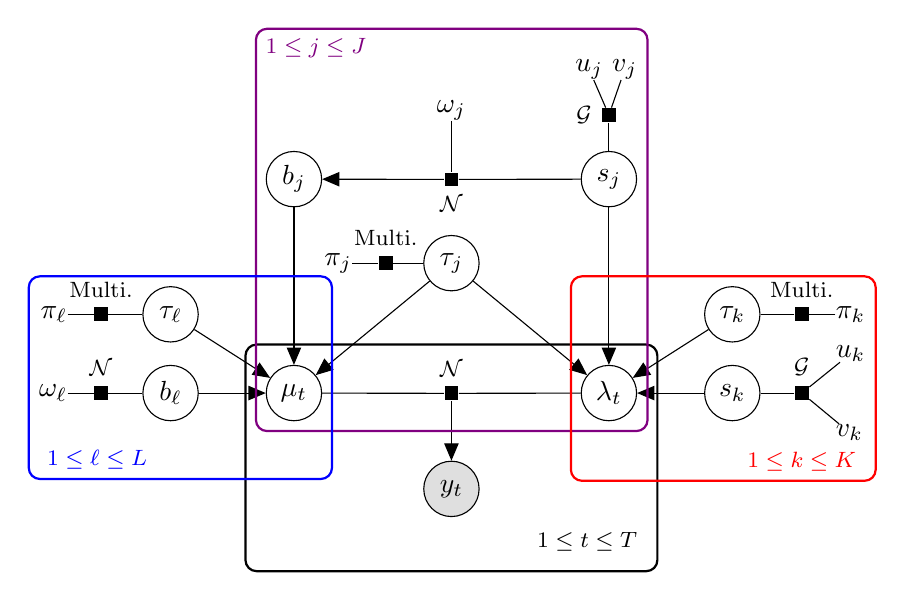
\begin{tikzpicture}[x=1.7cm,y=1.8cm]
  % Nodes

  % DGP
  \node[obs]                   (y)      {$y_t$} ; 
  \factor[above=0.76cm of y] {y-f} {above:$\mathcal{N}$} {} {} ; %
  \node[latent, above=0.5cm of y, xshift = -2cm]    (mu)     {$\mu_t$} ; 
  \node[latent, above=0.5cm of y, xshift = 2cm]    (lambda) {$\lambda_t$} ; 

  % SMCP
  \node[latent, left=0.5 of mu] (b_l) {$b_\ell$} ;
  \factor[left=of b_l, xshift=0.25cm] {b_l-f} {above:$\mathcal{N}$} {} {} ; %
  \node[const, left=of b_l, xshift=0.75cm] (tau_l) {$\omega_\ell$} ; %

  \node[latent, left=0.5 of mu, yshift=1cm] (gamma_l) {$\tau_\ell$} ;
  \factor[left=of gamma_l, xshift=0.25cm] {gamma_l-f} {above:Multi.} {} {} ; %
  \node[const, left=of gamma_l, xshift=0.75cm] (pi_l) {$\pi_\ell$} ; %

  % SSCP
  \node[latent, right=0.5 of lambda] (s_k) {$s_k$} ;
  \factor[right=of s_k, xshift=-0.25cm] {s_k-f} {above:$\mathcal{G}$} {} {} ; %
  \node[const, right=of s_k, xshift=-0.75cm, yshift = 0.5cm] (u_k) {$u_k$} ; %
  \node[const, right=of s_k, xshift=-0.75cm, yshift = -0.5cm] (v_k) {$v_k$} ; %

  \node[latent, right=0.5 of lambda, yshift=1cm] (gamma_k) {$\tau_k$} ;
  \factor[right=of gamma_k, xshift=-0.25cm] {gamma_k-f} {above:Multi.} {} {} ; %
  \node[const, right=of gamma_k, xshift=-0.75cm] (pi_k) {$\pi_k$} ; %

  % SMSCP
  \node[latent, above=2cm of mu] (b_j) {$b_j$} ;
  \node[latent, above=2cm of lambda] (s_j) {$s_j$} ;
  \factor[above=0.2 of s_j, xshift=0cm] {s_j-f} {left:$\mathcal{G}$} {} {} ; %
  \node[const, above=0.5 of s_j, xshift=-0.25cm] (u_j) {$u_j$} ; %
  \node[const, above=0.5 of s_j, xshift=0.2cm] (v_j) {$v_j$} ; %
  
  \node[latent, above=1.2cm of y-f] (gamma_j) {$\tau_j$} ;
  \factor[above=0.61cm of gamma_j] {b_j-f} {below:$\mathcal{N}$} {} {} ; %
  \node[const, above=0.65cm of b_j-f] (tau_j) {$\omega_j$} ; %
  \factor[left=of gamma_j , xshift=0.3cm] {gamma_j-f} {above:Multi.} {} {} ; %
  \node[const, left=of gamma_j, xshift=0.8cm] (pi_j) {$\pi_j$} ; %

  % Connect the nodes
  \edge {y-f} {y} ;
  \edge[-] {mu, lambda} {y-f} ; %

  \edge{gamma_l, b_l} {mu}
  \edge[-] {b_l-f} {b_l} ; %
  \edge[-] {gamma_l-f} {gamma_l} ; %
  \edge[-] {tau_l} {b_l-f} ; %
  \edge[-] {pi_l} {gamma_l-f} ; %

  \edge{gamma_k, s_k} {lambda}
  \edge[-] {s_k-f} {s_k} ; %
  \edge[-] {gamma_k-f} {gamma_k} ; %
  \edge[-] {u_k, v_k} {s_k-f} ; %
  \edge[-] {pi_k} {gamma_k-f} ; %

  
  \edge{gamma_j, b_j} {mu}
  \edge{b_j-f} {b_j} ; %
  \edge[-] {tau_j,s_j} {b_j-f} ; %
  \edge[-] {gamma_j-f} {gamma_j} ; %
  \edge[-] {pi_j} {gamma_j-f} ; %
  \edge{gamma_j, s_j} {lambda}
  \edge[-] {s_j-f} {s_j} ; %
  \edge[-] {u_j, v_j} {s_j-f} ; %
  
  % Plates
  \plate[thick, inner sep=.25cm]{y} {(y)(mu)(lambda)} {$1 \leq t \leq T$} ;
  \tikzset{plate caption/.append style={above right =0pt of #1.north west}}
  \plate[thick,color=violet]{mu lambda} {(mu)(lambda)(gamma_j)(gamma_j-f)(pi_j)(b_j)(b_j-f)(tau_j)(s_j)(s_j-f)(u_j)(v_j)}{\textcolor{violet}{$1 \leq j \leq J$}} ;
  \tikzset{plate caption/.append style={below left = 5pt of #1.south east}}
  \plate[thick,color=red]{lambda} {(lambda)(gamma_k)(gamma_k-f)(pi_k)(s_k)(s_k-f)(u_k)(v_k)}{\textcolor{red}{$1 \leq k \leq K$}} ;
  \tikzset{plate caption/.append style={below=10pt of #1.south west, xshift=0.75cm}}
  \plate[thick,color=blue]{mu} {(mu)(gamma_l)(gamma_l-f)(pi_l)(b_l)(b_l-f)(tau_l)}{\textcolor{blue}{$1 \leq \ell \leq L$}} ;
\end{tikzpicture}
    \caption{Plate diagram depicting the directed acyclic graph specified by (\ref{eq:dgp}) and (\ref{eq:mich-start})-(\ref{eq:lambda_t}).}
    \label{fig:plate-diagram}
\end{figure}  

\subsection{Fitting MICH}

The prior distributions specified in each of the SCP models from Section \ref{sec:scp} are conditionally conjugate; therefore, constructing a Gibbs sampler (\citealp{Geman84}) is a straightforward exercise. The problem with taking an MCMC approach to inference in this setting is that the change-point indicators $\{\gamma_j,\gamma_\ell,\gamma_k\}$ are discrete, highly correlated, and live in a high-dimensional space as $J$, $K$, $L$ and $T$ increase. Gibbs sampling will suffer from poor mixing under these conditions and the sampler may fail to converge, even after a large number of iterations (\citealp{Smith93, Cappello21}). To circumvent the challenges associated with MCMC based inference, we design an analytically tractable backfitting procedure (\citealp{Friedman81, Breiman85}) that approximates the posterior distribution implied by MICH. The backfitting procedure is described in detail in Algorithm \ref{alg:1}. Upon convergence, Algorithm \ref{alg:1} returns a distribution $q$ and in Section \ref{sec:variational-bayes} we show that Algorithm \ref{alg:1} is a variational Bayesian method, meaning that this $q$ is the best available approximation to the true posterior of MICH within a known class of distributions. 

To motivate the backfitting procedure in Algorithm \ref{alg:1}, consider the residual term:
\begin{align}\label{eq:residual}
    r_t &:= y_t - \sum_{j = 1}^J \mu_{jt}  - \sum_{\ell = 1}^L \mu_{\ell t}.
\end{align}
Note that the intercept $\mu_0$ does not appear in (\ref{eq:residual}). If we take $\mu_0$ and $\lambda_0$ as known constants, then by centering and rescaling $\mathbf{y}$, we can assume without loss of generality that $\mu_0 = 0$ and $\lambda_0=1$. For the case of unknown $\mu_0$ or $\lambda_0$, we estimate the missing parameter with an empirical Bayes procedure (see Appendix \ref{app:empirical-bayes} for details). Suppose for the moment that we have access to all of the MICH model parameters except for the block $\theta_j$. Then we can calculate both a mean and scale partial residual:
\begin{align}
    r_{-jt} &:= r_t + \mu_{jt \label{eq:smscp-mean-resid}} \\
    \lambda_{-jt} &:= \lambda_{jt}^{-1}\lambda_t. \label{eq:smscp-var-resid}
\end{align}
The exact posterior distribution for $\theta_j$ conditional on the other MICH parameters would be the SMSCP posterior returned by:
\begin{align}
    \texttt{SMSCP}(\mathbf{r}_{-j}\:;\: \pmb{\lambda}_{-j}, \tau_j, u_j, v_j, \pmb{\pi}_j, B_l,B_r).
\end{align}
Similarly, if we knew all of the MICH model parameters except for either $\theta_\ell$ or $\theta_k$, we could calculate the respective mean and scale partial residuals: 
\begin{align}
    r_{-\ell t} &:= r_t + \mu_{\ell t} \label{eq:smcp-resid}\\
    \lambda_{-kt} &:= \lambda_{kt}^{-1}\lambda_t. \label{eq:sscp-resid}
\end{align}
In each case, the posterior distributions for $\theta_\ell$ and $\theta_k$ conditional on the known model parameters would be the respective SMCP and SSCP posteriors returned by:
\begin{gather}
    \texttt{SMCP}(\mathbf{r}_{-\ell}\:;\: \pmb{\lambda}, \tau_\ell,\pmb{\pi}_\ell, B_l,B_r) \label{eq:smcp-call} \\
    \texttt{SSCP}(\mathbf{r}\:;\: \pmb{\lambda}_{-k}, u_k,v_k,\pmb{\pi}_k, B_l,B_r). \label{eq:sscp-call}
\end{gather}
The challenge of course is that we do not have access to any of the model parameters, so none of the partial residuals defined in (\ref{eq:smscp-mean-resid}), (\ref{eq:smscp-var-resid}), (\ref{eq:smcp-resid}), or (\ref{eq:sscp-resid}) can be calculated in practice. However, if we have initial approximations to the model parameters, then we can: i) calculate the partial residuals using the approximate parameters, ii) fit the appropriate SCP model using the partial residuals iii) update the approximate parameters using the fitted models. At a high level, Algorithm \ref{alg:1} iteratively repeats these three steps until some convergence criterion is met.

Let $q_j$, $q_\ell$, and $q_k$ be the respective approximate marginal posterior distributions for the blocks $\theta_j$, $\theta_\ell$, and $\theta_k$. For each $j$, $\ell$, and $k$, we initialize $q_j$, $q_\ell$, and $q_k$ by picking initial values for the parameters $\{\overline{b}_{jt}, \overline{\tau}_{jt}, \overline{u}_{jt}, \overline{v}_{jt}, \overline{\pi}_{jt}\}_{t=1}^T$, $\{\overline{b}_{\ell t}, \overline{\tau}_{\ell t}, \overline{\pi}_{\ell t}\}_{t=1}^T,$ and $\{\overline{u}_{kt}, \overline{v}_{kt}, \overline{\pi}_{kt}\}_{t=1}^T,$ and assuming that:
\begin{align}
    \theta_j &\sim \text{SMSCP}(\{\overline{b}_{jt}, \overline{\tau}_{jt}, \overline{u}_{jt}, \overline{v}_{jt}, \overline{\pi}_{jt}\}_{t=1}^T) \label{eq:q-j}\\
    \theta_\ell &\sim \text{SMCP}(\{\overline{b}_{\ell t}, \overline{\tau}_{\ell t}, \overline{\pi}_{\ell t}\}_{t=1}^T)\\
    \theta_k &\sim \text{SSCP}(\{\overline{u}_{kt}, \overline{v}_{kt}, \overline{\pi}_{kt}\}_{t=1}^T). \label{eq:q-k}
\end{align}
We also make the simplifying assumption that each of the parameter blocks $\theta_j$, $\theta_\ell$, and $\theta_k$ are independent in our approximation:
\begin{align}\label{eq:indep-blocks}
    q(\{\theta_j\}_{j=1}^J, \{\theta_\ell\}_{\ell=1}^L, \{\theta_k\}_{k=1}^K) := \prod_{j=1}^J q_j(\theta_j) \prod_{\ell=1}^L q_\ell(\theta_\ell) \prod_{k=1}^K q_k(\theta_k).
\end{align}
The independence assumption in (\ref{eq:indep-blocks}) is strong, but it is the key to unlocking the backfitting procedure in Algorithm \ref{alg:1}. Despite rendering the component blocks of MICH independent, assumption (\ref{eq:indep-blocks}) still allows for arbitrary dependencies within each block of parameters. This ability to characterize the relationship between the change-point indicator $\gamma$ and the rest of the variables in the block is what allows MICH to effectively localize the change-points. We will see in Section \ref{sec:variational-bayes} that (\ref{eq:indep-blocks}) constitutes a mean-field assumption in the context of variational inference. Let $\E_{g} [\:\cdot\:]$ denote the expectation taken with respect to a generic distribution $g$, then we define a modified residual term:
\begin{align}\label{eq:mod-resid}
    \tilde{r}_t &:= y_t - \sum_{j = 1}^J \frac{\E_{q_j}[\lambda_{jt} \mu_{jt}]}{\E_{q_j}[\lambda_{jt}]}  - \sum_{\ell = 1}^L \E_{q_\ell}[\mu_{\ell t}].
\end{align}
In Algorithm \ref{alg:1}, we use $\tilde{r}_t$ as a stand in for $r_t$ and calculate partial residuals analogous to (\ref{eq:smscp-mean-resid}) and (\ref{eq:smcp-resid}):
\begin{align}
    \tilde{r}_{-jt} &:= \tilde{r}_t + \frac{\E_{q_j}[\lambda_{jt} \mu_{jt}]}{\E_{q_j}[\lambda_{jt}]} \label{eq:smscp-mean-e-resid} \\
    \tilde{r}_{-\ell t} &:= \tilde{r}_t + \E_{q_\ell}[\mu_{\ell t}]. \label{eq:smcp-e-resid} 
\end{align}
Similarly, we define an expected precision vector as a stand in for $\lambda_t$:
\begin{align}\label{eq:lambda-bar}
    \overline{\lambda}_t &:= \prod_{j=1}^J \E_{q_j}[\lambda_{jt}] \prod_{k=1}^K \E_{q_k}[\lambda_{kt}]
\end{align}
and define partial the analogous partial residuals to (\ref{eq:smscp-var-resid}) and (\ref{eq:sscp-resid}):
\begin{align}
    \overline{\lambda}_{-jt} &:= \E_{q_j}[\lambda_{jt}]^{-1}\overline{\lambda}_{t} \label{eq:smscp-var-e-resid}  \\
    \overline{\lambda}_{-kt} &:= \E_{q_k}[\lambda_{kt}]^{-1}\overline{\lambda}_{t}. \label{eq:sscp-e-resid}
\end{align}
Given initial estimates of the model parameters, the backfitting procedure in Algorithm \ref{alg:1} proceeds by iteratively fitting the appropriate SCP model to the partial residuals defined in (\ref{eq:smscp-mean-e-resid}), (\ref{eq:smscp-var-e-resid}), (\ref{eq:smcp-e-resid}), and (\ref{eq:sscp-e-resid}), then updating the model parameters using the fitted models.

An important difference between Algorithm \ref{alg:1} and other backfitting procedures is that (\ref{eq:mod-resid}) is not exactly equal to $\E_q[r_t]$, which is the residual term typically used when backfitting models with additive effects (\citealp{Breiman85,Hastie90,Friedman00,Wang20}). Rather, we have $\E_q[\lambda_t r_t] = \overline{\lambda}_t \tilde{r}_t$. Our choice to use (\ref{eq:mod-resid}) instead of $\E_q[r_t]$ is necessitated by the inclusion of both additive and multiplicative effects in MICH, a fact that will become clear in the derivation of Algorithm \ref{alg:1} in Appendix \ref{app:prop1-proof}. We also must define a variance correction term:
\begin{align}\label{eq:delta}
    \delta_t &:= \sum_{j=1}^J\left(\frac{\E_{q_j}[\lambda_{jt} \mu^2_{jt}]}{\E_{q_j}[\lambda_{jt}]} -\frac{\E_{q_j}[\lambda_{jt} \mu_{jt}]^2}{\E_{q_j}[\lambda_{jt}]^2} \right) +\sum_{\ell=1}^L  \Var_{q_\ell}\left(\mu_{\ell t} \right).
\end{align}
The correction term $\pmb{\delta} = \{\delta_{t}\}_{t=1-B_l}^{B_r}$ plays an important role in Algorithm \ref{alg:1} that did not previously appear in either the IBSS algorithm of \cite{Wang20} or the ProSCALE algorithm of \cite{Cappello22}. After defining the mean and scale partial residuals as in (\ref{eq:smcp-resid}) and (\ref{eq:sscp-resid}), IBSS and ProSCALE take the expectation with respect to $q$ and iteratively update the parameters of each $\theta_\ell$ and $\theta_k$ block by making a call to \texttt{SMCP} and \texttt{SSCP} with the respective expected partial residuals. In other words, they make the calls defined in (\ref{eq:smcp-call}) and (\ref{eq:sscp-call}), but with the expected analogs of $\mathbf{r}_{-\ell}$ and $\pmb{\lambda}_{-\ell}$. The procedure in Algorithm \ref{alg:1} is similar, but as we will see in Section \ref{sec:variational-bayes}, in order to maintain the validity of Algorithm \ref{alg:1} as a variational Bayes procedure, we must apply a correction to the priors on $s_j$ and $s_k$ using $\pmb{\delta}$. We then call \texttt{SMSCP} and \texttt{SSCP} with the corrected priors (see lines 9 and 29 of Algorithm \ref{alg:1} for more detail detail). 

Due to our choice of $q$ in (\ref{eq:q-j})-(\ref{eq:indep-blocks}), each of the expectation terms in (\ref{eq:mod-resid}) and (\ref{eq:lambda-bar}) have closed forms in terms of the parameters in (\ref{eq:q-j})-(\ref{eq:q-k}) (see Appendix \ref{app:prop1-proof} for details). The availability of these closed form solutions in addition to the backfitting procedure make Algorithm \ref{alg:1} computationally simple. During the backfitting steps, each call of $\texttt{SMCP}$, $\texttt{SSCP}$, and $\texttt{SMSCP}$  requires the calculation of a cumulative sum with $T$ terms, which is an order $\mathcal{O}(T)$ operation. Thus, each iteration of Algorithm \ref{alg:1} is order $\mathcal{O}((J+K+L)T)$. The number of iterations is itself indeterminate and will depend on the convergence criterion unless a maximum number of iterations is specified. We discuss the choice of stopping rule in greater detail in Appendix \ref{app:convergence}.  

\begin{algorithm}
\label{alg:1}
\caption{Variational Bayes Approximation to MICH Posterior.}

\footnotesize
\SetAlgoLined
  Inputs: $L,\:K,\:J,\:\{\tau_\ell,\pi_\ell\}_{\ell=1}^L,\:\{u_k,v_k,\pi_k\}_{k=1}^K,\:\{\tau_j,u_j,v_j,\pi_j\}_{j=1}^J;$ \\
  Initialize: $\overline{\boldsymbol{\Theta}} := \{\{\overline{\boldsymbol{\theta}}_\ell\}_{\ell=1}^L$, $\{\overline{\boldsymbol{\theta}}_k\}_{k=1}^K$, $\{\overline{\boldsymbol{\theta}}_j\}_{j=1}^J\}$;
  
  \Repeat {Convergence} {
    \For{$\ell=1$ \KwTo $L$} {
      $\tilde{r}_{-\ell t} := y_t - \sum_{\ell' \neq \ell}^L \E[\mu_{\ell' t}] - \sum_{j =1}^J \E[\lambda_{jt} \mu_{jt}] / \E[\lambda_{jt}]$ \tcp*{l\textsuperscript{th} partial mean residual}
      $\overline{\lambda}_{t} := \prod_{k=1}^K \E[\lambda_{kt}]\prod_{j=1}\E[\lambda_{jt}]$ \tcp*{precision of residual} 
      $\overline{\boldsymbol{\theta}}_\ell := \texttt{mean-scp}(\tilde{\mathbf{r}}_{-\ell} \:;\: \overline{\boldsymbol{\lambda}}_{1:T}, \tau_{\ell}, \boldsymbol{\pi}_{\ell})$ \tcp*{update mean parameters}
    }
    \For{$k=1$ \KwTo $K$} {
      $\tilde{r}_{t} := y_t - \sum_{\ell = 1}^L \E[\mu_{\ell t}] - \sum_{j=1}^J \E[\lambda_{jt} \mu_{jt}] / \E[\lambda_{jt}]$ \tcp*{mean residual} 
      $\overline{\lambda}_{-kt} := \prod_{k' \neq k} \E[\lambda_{k't}]\prod_{j=1}^J\E[\lambda_{jt}] $ \tcp*{k\textsuperscript{th} partial scale residual} 
      %% $\delta_{t} := \sum_{\ell=1}^L  \Var(\mu_{\ell t} ) + \sum_{j=1}^J[\E[\lambda_{jt} \mu^2_{jt}] / \E[\lambda_{jt}] - (\E[\lambda_{jt} \mu_{jt}] / \E[\lambda_{jt}])^2 ];$ \tcp*{variance correction term}\\
      Compute $\boldsymbol{\delta}_{1:T}$, $\tilde{\mathbf{v}}_{k}$, and $\tilde{\boldsymbol{\pi}}_{k}$ by (\ref{eq:delta}), (\ref{eq:mod-v_k}), and (\ref{eq:mod-pi_k}) \tcp*{variance corrected priors} 
      $\overline{\boldsymbol{\theta}}_k := \texttt{var-scp}(\tilde{\mathbf{r}}_{1:T} 
      \:;\:\overline{\boldsymbol{\lambda}}_{-k}, u_k, \tilde{\mathbf{v}}_{k}, \tilde{\boldsymbol{\pi}}_k)$ \tcp*{update var parameters}
    }
    \For{$j=1$ \KwTo $J$} {
      $\tilde{r}_{-jt} := y_t - \sum_{\ell = 1}^L \E[\mu_{\ell t}] - \sum_{j' \neq j} \E[\lambda_{j't} \mu_{j't}] / \E[\lambda_{j't}]$ \tcp*{j\textsuperscript{th} partial mean residual} 
      $\overline{\lambda}_{-jt} := \prod_{k=1}^K \E[\lambda_{kt}]\prod_{j' \neq j}\E[\lambda_{j't}] $ \tcp*{j\textsuperscript{th} partial scale residual}
      %%$\delta_{-jt} := \sum_{\ell=1}^L  \Var(\mu_{\ell t} ) + \sum_{j' \neq j}[\E[\lambda_{j't} \mu^2_{j't}] / \E[\lambda_{j't}] - (\E[\lambda_{j't} \mu_{j't}] / \E[\lambda_{j't}])^2 ]$ \tcp*{j\textsuperscript{th} variance correction term} 
      Compute $\boldsymbol{\delta}_{-j}$, $\tilde{\mathbf{v}}_{j}$, and $\tilde{\boldsymbol{\pi}}_{j}$ by (\ref{eq:delta_j}), (\ref{eq:mod-v_j}), and (\ref{eq:mod-pi_j}) \tcp*{variance corrected priors} 
      $\overline{\boldsymbol{\theta}}_j := \texttt{meanvar-scp}(\tilde{\mathbf{r}}_{-j} \:;\:\overline{\boldsymbol{\lambda}}_{-j}, \tau_j, u_j, \tilde{\mathbf{v}}_{j}, \tilde{\boldsymbol{\pi}}_j)$ \tcp*{update meanvar parameters}
    }
  }
  \Return{Posterior Parameters: $\overline{\boldsymbol{\Theta}}$}.
\end{algorithm}

Upon convergence, Algorithm \ref{alg:1} returns estimates for the posterior probabilities of the change-point locations. For each $j$, $\ell$, and $k$, we can construct MAP estimators for the change-point locations as in (\ref{eq:map}):
\begin{align}\label{eq:multi-map}
    \hat{t}_{\text{MAP}, i} := \argmax{1 \leq t \leq T} \; \overline{\pi}_{it}, \quad i \in \{j, \ell, k\}.
\end{align}
We can also construct $\alpha$-level credible sets around each $\hat{t}_{\text{MAP}, i}$ as in (\ref{eq:cs}):
\begin{align}\label{eq:multi-cs}
    \mathcal{CS}(\alpha, \overline{\pmb{\pi}}_i) := \argmin{S \subset \{1,\ldots,T\}} |S| \quad\text{ s.t. } \sum_{t \in S} \overline{\pi}_{it} \geq \alpha, \quad i \in \{j, \ell, k\}.
\end{align}
The MAP estimator in (\ref{eq:multi-map}) and credible set in (\ref{eq:multi-cs}) will still be well-defined even if the index $i$ does not correspond to a true change-point. This will be the case for some $i$ if we fit MICH with $J$, $L$, or $K$ set greater than the corresponding true number of change-points. However, as was the case with a single-change point in Section \ref{sec:localization}, the elements of $\overline{\pmb{\pi}}_i$ tend to be diffuse when the index $i$ does not capture a true change-point. This motivates a generalization  of the heuristic detection rule from \cite{Cappello22}, whereby we only detect a change-point if its associated credible set contains $T/2$ or fewer locations. Adopting this detection rule also gives the following estimators for the numbers of each kind of change-point:
\begin{align}
    \hat{J} &:= |\{j \;:\; j \in \{1,\ldots,J\}, \;\;|\mathcal{CS}(\alpha, \overline{\pmb{\pi}}_j)| \leq T/2\}| \label{eq:J-estimator}\\
    \hat{L} &:= |\{\ell \;:\; \ell \in \{1,\ldots,L\},\;\;\: |\mathcal{CS}(\alpha, \overline{\pmb{\pi}}_\ell)| \leq T/2\}| \label{eq:L-estimator}\\
    \hat{K} &:= |\{k \;:\; k \in \{1,\ldots,K\},\; |\mathcal{CS}(\alpha, \overline{\pmb{\pi}}_k)| \leq T/2\}|. \label{eq:K-estimator}
\end{align}

\subsection{MICH as a Mean-Field Variational Approximation}
\label{sec:variational-bayes}

In this section we show that the distribution $q$ returned by Algorithm \ref{alg:1} constitutes a variational approximation to the posterior implied by the MICH model. Proposition \ref{prop:1} and Corollary \ref{cor:1} establish the validity of Algorithm \ref{alg:1} as a variational Bayesian (VB) procedure, while Proposition \ref{prop:2} establishes the convergence of Algorithm \ref{alg:1}. These three results are the respective analogs of Proposition 1, Corollary 1, and Proposition 2 in \cite{Wang20}. For a review of VB methods we refer the reader to the classical treatment in \cite{Jordan99} and the recent review in \cite{Blei17}. We begin by considering the generic model:
\begin{align}
    \mathbf{y} \:|\: \theta &\sim f(\mathbf{y}\:|\: \theta;\eta) \\
    \theta &\sim g(\theta)
\end{align}
where the nuisance parameter $\eta$ in the likelihood of $\mathbf{y}$ is taken as known. The goal of VB inference is to find a distribution $q^*(\theta)$ that is the closest approximation to the true posterior $p(\theta\:|\: \mathbf{y};\eta)$ as measured by the Kullback–Leibler divergence (\citealp{Kullback51}):
\begin{align}\label{eq:unrestriced-kl}
    q^* := \argmin{q}  \; \text{KL}( q(\theta) \:\lVert\: p(\theta\:|\: \mathbf{y};\eta)).
\end{align}
If we knew the exact form of $p(\theta\:|\: \mathbf{y};\eta)$, then we could solve (\ref{eq:unrestriced-kl}) by simply setting $q^*(\theta)\equiv p(\theta\:|\: \mathbf{y};\eta)$, in which case the KL-divergence would achieve its zero lower-bound. However, in cases such as ours where there is no closed form available for the posterior, we must resort to computational methods to find $q^*$. Because the minimization in (\ref{eq:unrestriced-kl}) is taken with respect to all possible distributions over $\theta$, finding a solution computationally is generally an impossible task. Therefore, we restrict $q^*$ to a known family of distributions $\mathcal{Q}$ that we hope will simplify the problem:
\begin{align}\label{eq:restriced-kl}
    q^* := \argmin{q\in\mathcal{Q}}  \; \text{KL}( q(\theta) \:\lVert\: p(\theta\:|\: \mathbf{y};\eta)).
\end{align}
In many applications, we can naturally partition $\theta$ into a finite number of blocks $\theta = \{\theta_1, \ldots, \theta_M\}$.\footnote{Examples include product partition models (\citealp{Hartigan90, Barry92}), stochastic block models (\citealp{Holland83}), and mixture models (\citealp{Corduneanu01}).} In such cases, one intuitive way to structure $\mathcal{Q}$ and $g$ is:
\begin{align} 
    \mathcal{Q} &= \left\{q \::\: q(\theta) = \prod_{i=1}^M q_i(\theta_i)\right\}, \label{eq:mfvb} \\
    g(\theta) &= \prod_{i=1}^M g_i(\theta_i) \label{eq:ind-prior}
\end{align}
i.e. we restrict the approximate posterior $q$ and the prior $g$ to families of distributions that render the $M$ blocks of $\theta$ independent. Restrictions of the form (\ref{eq:mfvb}) are called mean-field assumptions and are very common within the VB literature due to the fact that they often lead to analytic solutions for (\ref{eq:restriced-kl}) (\citealp{Wainright08}). In particular, for MICH we have:
\begin{align}
    \theta &:= \left\{\{\theta_j\}_{j=1}^J, \{\theta_\ell\}_{\ell=1}^L,\{\theta_k\}_{k=1}^K\right\} \\
    \eta &:= \{\mu_0,\lambda_0\}
\end{align}
and we make the mean-field assumption:
\begin{align}
    \mathcal{Q} := \left\{q \;:\; q\left(\theta\right) = \prod_{j=1}^J q_j(\theta_j) \prod_{\ell=1}^L q_\ell(\theta_\ell)\prod_{k=1}^K q_k(\theta_k)\right\}.\label{eq:mean-field}
\end{align}
Note that the distribution we defined in (\ref{eq:q-j})-(\ref{eq:indep-blocks}) belongs to $\mathcal{Q}$, meaning that we already know the distribution returned by Algorithm \ref{alg:1} is at least a candidate solution to (\ref{eq:restriced-kl}). In addition to restricting the solution to $\mathcal{Q}$, the minimization problem in (\ref{eq:restriced-kl}) can often be simplified even further by using the following equivalent characterization of the KL-divergence: 
\begin{align}
     \text{KL}( q(\theta) \:\lVert\: p(\theta\:|\: \mathbf{y};\eta)) &= \log \int f(\mathbf{y}\:|\:\theta;\eta)g(\theta)\;d\theta - \int q(\theta) \log \frac{ f(\mathbf{y}\:|\: \theta;\eta) g(\theta)}{q(\theta)} \; d\theta. \label{eq:kl-decomp} 
\end{align}
Because the KL-divergence is non-negative for all choices of $q$, by (\ref{eq:kl-decomp}) we have:
\begin{align}\label{eq:elbo}
    \text{ELBO}(q;\eta) := \int q(\theta) \log \frac{ f(\mathbf{y}\:|\: \theta;\eta) g(\theta)}{q(\theta)} \; d\theta \leq \log \int f(\mathbf{y}\:|\:\theta;\eta)g(\theta)\;d\theta.
\end{align}
The log-marginal likelihood that appears in the upper bound of (\ref{eq:elbo}) is frequently referred to as the log-evidence, and thus the term on the left-hand side of the inequality is called the evidence lower bound (ELBO). Notably, the log-evidence does not depend on $q$, so by (\ref{eq:kl-decomp}) solving (\ref{eq:restriced-kl}) is equivalent to solving: 
\begin{align}
    \label{eq:restriced-elbo}
    q^* := \argmax{q\in\mathcal{Q}}  \; \text{ELBO}(q;\eta).
\end{align}
We can now show that the distribution returned by Algorithm \ref{alg:1} is an approximation to the precise $q^*$ we seek in (\ref{eq:restriced-elbo}). In the statement of this result, we use the following non-standard notation for the distribution $q$ with the $i^{\text{th}}$ parameter block marginalized out:
\begin{align}
    q_{-i}(\theta_{-i}) &:= \int q(\theta) \; d\theta_i. \label{eq:q-minus-i}
\end{align}
When $q \in \mathcal{Q}$, we simply have $q_{-i}(\theta_{-i}) =q_{i}(\theta_{i})^{-1}q(\theta)$. We are now ready to state our main result.
\begin{proposition} 
\label{prop:1}
Let $p(\theta\:|\: \mathbf{y};\eta)$ be the posterior of the MICH model and define the terms $\tilde{r}_{t}$, $\overline{\lambda}_t$, and $\delta_t$ as in (\ref{eq:mod-resid}), (\ref{eq:lambda-bar}), and (\ref{eq:delta}) respectively.
\begin{enumerate}[label=\roman*.]
    \item Let $q_{-j}(\theta_{-j})$ be a known distribution. For all $t$, define $\tilde{r}_{-jt}$ as in (\ref{eq:smscp-mean-e-resid}) and $\overline{\lambda}_{-jt}$ as in (\ref{eq:smscp-var-e-resid}). If we define a partial correction term:
    \begin{align}
        \delta_{-jt} &:= \delta_t - \frac{\E_{q_j}[\lambda_{jt} \mu^2_{jt}]}{\E_{q_j}[\lambda_{jt}]} + \frac{\E_{q_j}[\lambda_{jt} \mu_{jt}]^2}{\E_{q_j}[\lambda_{jt}]^2}
    \end{align}
    and use $\delta_{-jt}$ to define a corrected prior rate parameter for $s_k$ and a corrected prior probability for the $j^{\text{th}}$ change-point location as:
    \begin{align}
        \tilde{v}_{jt} &:= v_j + \frac{1}{2}\sum_{t'=t}^{T+B_r}\overline{\lambda}_{-jt'}\delta_{-jt'} \label{eq:mod-v_j} \\
        \tilde{\pi}_{jt} &:= \frac{\pi_{jt} \exp\left(-\frac{1}{2}\sum_{t'=1}^{t-1}\overline{\lambda}_{-jt'}\delta_{-jt'}\right)}{\sum_{t'=1}^T \pi_{jt'} \exp\left(-\frac{1}{2}\sum_{t''=1}^{t'-1}\overline{\lambda}_{-jt''}\delta_{-jt''}\right)} \label{eq:mod-pi_j}
    \end{align}
    then the maximization problem:
    \begin{align}
        \normalfont
        \max_{q_j} \; \text{ELBO}(q_j(\theta_j)q_{-j}(\theta_{-j}) \:;\: \eta)\label{eq:elbo-j}
    \end{align}
    is solved by choosing $q_j$ so that: 
    \begin{align*}
        \normalfont
        \theta_j \sim \text{SMSCP}(\{\overline{b}_{jt}, \overline{\tau}_{jt}, \overline{u}_{jt}, \overline{v}_{jt}, \overline{\pi}_{jt}\}_{t=1}^T)
    \end{align*}
    where 
    \begin{align*}
        \normalfont
        \{\overline{b}_{jt}, \overline{\tau}_{jt}, \overline{u}_{jt}, \overline{v}_{jt}, \overline{\pi}_{jt}\}_{t=1}^T = \texttt{SMSCP}(\tilde{\mathbf{r}}_{-j} \:;\:\overline{\pmb{\lambda}}_{-j}, \tau_j, u_j, \tilde{\mathbf{v}}_j, \tilde{\pmb{\pi}}_j, B_l,B_r).
    \end{align*}

    \item Let $q_{-\ell}(\theta_{-\ell})$ be a known distribution. For all $t$, define define $\tilde{r}_{-\ell t}$ as in (\ref{eq:smcp-e-resid}). Then the maximization problem:
    \begin{align}
        \normalfont
        \max_{q_\ell} \; \text{ELBO}(q_\ell(\theta_\ell)q_{-\ell}(\theta_{-\ell}) \:;\: \eta) \label{eq:elbo-l}
    \end{align}
    is solved by choosing $q_\ell$ so that: 
    \begin{align*}
        \normalfont
        \theta_\ell \sim \text{SMCP}(\{\overline{b}_{\ell t}, \overline{\tau}_{\ell t}, \overline{\pi}_{\ell t}\}_{t=1}^T)
    \end{align*}
    where 
    \begin{align*}
        \normalfont
        \{\overline{b}_{\ell t}, \overline{\tau}_{\ell t}, \overline{\pi}_{\ell t}\}_{t=1}^T= \texttt{SMCP}(\tilde{\mathbf{r}}_{-\ell t} \:;\: \overline{\pmb{\lambda}}_t, \tau_{\ell}, \pmb{\pi}_{\ell}, B_l,B_r).
    \end{align*}

    \item Let $q_{-k}(\theta_{-k})$ be a known distribution. For all $t$, define $\overline{\lambda}_{-kt}$ as in (\ref{eq:sscp-e-resid}). If we define a corrected prior rate parameter for $s_k$ and a corrected prior probability for the $k^{\text{th}}$ change-point location as:
    \begin{align}
        \tilde{v}_{kt} &:= v_k + \frac{1}{2}\sum_{t'=t}^{T+B_r}\overline{\lambda}_{-kt'}\delta_{t'} \label{eq:mod-v_k} \\
        \tilde{\pi}_{kt} &:= \frac{\pi_{kt} \exp\left(-\frac{1}{2}\sum_{t'=1}^{t-1}\overline{\lambda}_{-kt'}\delta_{t'}\right)}{\sum_{t'=1}^T \pi_{kt'} \exp\left(-\frac{1}{2}\sum_{t''=1}^{t'-1}\overline{\lambda}_{-kt''}\delta_{-kt''}\right)} \label{eq:mod-pi_k}
    \end{align}
    then the maximization problem:
    \begin{align}
        \normalfont
        \max_{q_k} \;\text{ELBO}(q_k(\theta_j)q_{-k}(\theta_{-k}) \:;\: \eta) \label{eq:elbo-k}
    \end{align}
    is solved by choosing $q_k$ so that: 
    \begin{align*}
        \normalfont
        \theta_k &\sim \normalfont \text{SSCP}(\{\overline{u}_{kt}, \overline{v}_{kt}, \overline{\pi}_{kt}\}_{t=1}^T)
    \end{align*}
    where 
    \begin{align*}
        \normalfont
        \{\overline{u}_{kt}, \overline{v}_{kt}, \overline{\pi}_{kt}\}_{t=1}^T = \texttt{SSCP}(\tilde{\mathbf{r}}_{t} \:;\: \overline{\pmb{\lambda}}_{-kt}, u_k, \tilde{\mathbf{v}}_{kt}, \tilde{\pmb{\pi}}_{kt}, B_l,B_r).
    \end{align*}
\end{enumerate}
\end{proposition}
The proof of Proposition \ref{prop:1} is given in Appendix \ref{app:prop1-proof}. Looking back, we see that Algorithm \ref{alg:1} begins by initializing some distribution $q \in \mathcal{Q}$, then proceeds to iteratively fix $q_{-i}(\theta_{-i})$, calculate the relevant residuals using $q_{-i}(\theta_{-i})$, and update $q_{i}(\theta_{i})$ by solving the appropriate maximization problem in (\ref{eq:elbo-j}), (\ref{eq:elbo-l}), or (\ref{eq:elbo-k}). In this sense, Algorithm \ref{alg:1} is a coordinate ascent procedure for solving the maximization problem in (\ref{eq:restriced-elbo}). We formalize this statement in Corollary \ref{cor:1}
\begin{corollary}
\label{cor:1} 
Let $\mathcal{Q}$ be defined as in (\ref{eq:mean-field}). Then by Proposition \ref{prop:1}, Algorithm \ref{alg:1} is a coordinate ascent procedure for finding the distribution $q^*$ that solves the maximization problem in (\ref{eq:restriced-elbo}). Equivalently, Algorithm \ref{alg:1} is a coordinate descent procedure for solving the minimization problem in (\ref{eq:restriced-kl}).
\end{corollary}
Proposition \ref{prop:1} in conjunction with Corollary \ref{cor:1} establish that the distribution returned by Algorithm \ref{alg:1} is a VB approximation to the true posterior of MICH. It still remains to confirm that Algorithm \ref{alg:1} will in fact converge. To see this, note that the distributions $q_j$, $q_\ell$, and $q_k$ that respectively solve (\ref{eq:elbo-j}), (\ref{eq:elbo-l}), or (\ref{eq:elbo-k}) are fully characterized by the sets of parameters returned by the each call to \texttt{SMSCP}, \texttt{SMCP}, or \texttt{SSCP}. Proposition \ref{prop:2} establishes that these parameters converge to a stationary point, and thus so will the distribution returned by Algorithm \ref{alg:1}. 
\begin{proposition}
\label{prop:2}
Assume that the MICH prior parameters: 
\begin{align*}
    \{\{\tau_j, u_j, v_j, \{\pi_{jt}\}_{t=1}^T\}_{j=1}^J, \{\tau_\ell,  \{\pi_{\ell t}\}_{t=1}^T\}_{\ell=1}^L, \{u_k, v_k, \{\pi_{kt}\}_{t=1}^T\}_{k=1}^K\}
\end{align*}
are all strictly positive. Then the sequence of parameters generated by each iteration of Algorithm \ref{alg:1}: 
\begin{align}\label{eq:alg1-params}
    \{\{\overline{b}_{jt}, \overline{\tau}_{jt}, \overline{u}_{jt}, \overline{v}_{jt}, \overline{\pi}_{jt}\}_{j=1}^J, \{\overline{b}_{\ell t}, \overline{\tau}_{\ell t}, \overline{\pi}_{\ell t}\}_{\ell=1}^L, \{\overline{u}_{kt}, \overline{v}_{kt}, \overline{\pi}_{kt}\}_{k=1}^K\}_{t=1}^T
\end{align}
converge to some limit point. Therefore, the sequence of distributions generate by Algorithm \ref{alg:1}, which are parameterized by (\ref{eq:alg1-params}), will converge to a stationary point of $\text{ELBO}(q\:;\eta)$.
\end{proposition}
The proof of Proposition \ref{prop:2} is given in Appendix \ref{app:prop2-proof}.

\subsection{Choice of \texorpdfstring{$J$}{J}, \texorpdfstring{$L$}{L}, and \texorpdfstring{$K$}{K}}

\section{Simulations}
\label{sec:simulations}

\textit{In Progress.}

In this section, we reproduce the simulation study from Section 4 of \cite{Pein17}, in which we generate $\mathbf{y}$ by:
\begin{enumerate}
    \item Fix the number of observations $T$, the number of change-points $L$, a constant $C=200$ and a minimum spacing condition.
    \item Draw the locations of the $L$ change-points uniformly from $\{2, \ldots, T-1\}$ subject to the minimum spacing condition. 
    \item Draw standard deviations $s_1, \ldots, s_L$ independently so that $s_\ell = 2^{U_\ell}$ where $U_\ell \sim \text{Uniform}(-2,2)$.
\end{enumerate}


\begin{table} \label{tab:hsmuce-sim}
    \footnotesize
    \centering
    \begin{tabular}{l| r r r r r r r r r r}
        Method & T & L & Min. Space & $|L - \hat{L}|$ & CI Len. & Cond. Cov. & $d(C^*,\hat{C})$ & FPSLE & FNSLE & Time \\ \hline\hline 
        H-SMUCE & 100 & 2 & 15 & 0.33 & 24.08 & 0.98 & 14.30 & 0.92 & 3.27 & 0.01 \\
        MICH(0,L,K) &  &  &  & 0.38 & 2.58 & 0.96 & 0.80 & 1.58 & 0.67 & 0.07 \\
        MICH(0,L,K) Oracle &  &  &  & 0.00 & 1.49 & 0.96 & 0.51 & 0.16 & 0.17 & 0.01 \\
        MICH(J,0,0) &  &  &  & 0.68 & 3.32 & 0.97 & 0.27 & 2.65 & 0.88 & 0.05 \\
        MICH(J,0,0) Oracle &  &  &  & 0.00 & 1.38 & 0.97 & 0.26 & 0.10 & 0.10 & 0.01 \\
        MOSUM BU &  &  &  & 0.13 & 9.26 & 0.97 & 2.84 & 0.99 & 0.99 & 0.01 \\
        MOSUM LP &  &  &  & 0.17 & 5.96 & 0.99 & 1.83 & 0.90 & 0.70 & 0.01 \\
        NOT &  &  &  & 0.16 & &  & 2.35 & 1.27 & 0.76 & 0.02 \\
        PELT &  &  &  & 0.12 & &  & 0.84 & 0.57 & 0.26 & 0.00\\ \hline
        
        H-SMUCE & 100 & 5 & 15 & 1.94 & 17.12 & 0.84 & 23.48 & 3.26 & 6.16 & 0.01 \\
        MICH(0,L,K) &  &  &  & 0.44 & 1.66 & 0.98 & 10.85 & 1.37 & 2.39 & 0.13 \\
        MICH(0,L,K) Oracle &  &  &  & 0.44 & 1.66 & 0.98 & 10.85 & 1.37 & 2.39 & 0.13 \\
        MICH(J,0,0) &  &  &  & 0.21 & 1.51 & 0.99 & 7.96 & 1.14 & 1.77 & 0.43 \\
        MICH(J,0,0) Oracle &  &  &  & 0.21 & 1.51 & 0.99 & 7.96 & 1.14 & 1.77 & 1.25 \\
        MOSUM BU &  &  &  & 0.78 & 24.12 & 1.00 & 13.41 & 1.12 & 2.23 & 0.02 \\
        MOSUM LP &  &  &  & 0.39 & 8.17 & 1.00 & 5.71 & 0.65 & 1.04 & 0.02 \\
        NOT &  &  &  & 0.32 &  &  & 6.45 & 0.58 & 0.76 & 0.02 \\
        PELT &  &  &  & 0.19 &  &  & 0.88 & 0.27 & 0.15 & 0.00\\ \hline

        H-SMUCE & 500 & 2 & 30 & 0.09 & 53.88 & 1.00 & 20.59 & 1.35 & 4.43 & 0.01 \\
        MICH(0,L,K) &  &  &  & 0.40 & 9.40 & 0.86 & 5.87 & 6.82 & 3.54 & 1.11 \\
        MICH(0,L,K) Oracle &  &  &  & 0.01 & 4.64 & 0.87 & 4.30 & 1.18 & 1.70 & 0.40 \\
        MICH(J,0,0) &  &  &  & 0.76 & 13.20 & 0.93 & 2.60 & 12.02 & 4.17 & 2.73 \\
        MICH(J,0,0) Oracle &  &  &  & 0.01 & 3.76 & 0.94 & 2.39 & 1.49 & 1.73 & 0.03 \\
        MOSUM BU &  &  &  & 0.40 & 24.00 & 0.98 & 4.78 & 11.64 & 5.26 & 0.02 \\
        MOSUM LP &  &  &  & 0.39 & 17.34 & 0.99 & 5.94 & 9.22 & 4.62 & 0.02 \\
        NOT &  &  &  & 0.04 &  &  & 4.25 & 1.42 & 1.15 & 0.04 \\
        PELT &  &  &  & 0.03 &  &  & 4.18 & 0.89 & 1.01 & 0.00\\ \hline 

        H-SMUCE & 500 & 5 & 15 & 0.60 & 40.17 & 0.92 & 25.92 & 1.96 & 6.37 & 0.01 \\
        MICH(0,L,K) &  &  &  & 1.02 & 6.33 & 0.91 & 16.89 & 6.67 & 7.03 & 8.07 \\
        MICH(0,L,K) Oracle &  &  &  & 0.51 & 5.25 & 0.91 & 44.65 & 7.14 & 14.71 & 0.64 \\
        MICH(J,0,0) &  &  &  & 1.70 & 8.93 & 0.95 & 4.72 & 9.79 & 3.43 & 4.35 \\
        MICH(J,0,0) Oracle &  &  &  & 0.18 & 3.88 & 0.95 & 24.17 & 5.18 & 8.33 & 3.83 \\
        MOSUM BU &  &  &  & 0.44 & 29.02 & 0.99 & 5.80 & 4.98 & 2.50 & 0.04 \\
        MOSUM LP &  &  &  & 0.63 & 16.04 & 1.00 & 15.51 & 5.66 & 5.05 & 0.03 \\
        NOT &  &  &  & 0.08 &  &  & 5.49 & 0.90 & 0.78 & 0.05 \\
        PELT &  &  &  & 0.06 &  &  & 3.53 & 0.61 & 0.53 & 0.00\\ \hline 

        H-SMUCE & 1000 & 2 & 50 & 0.04 & 90.55 & 1.00 & 12.11 & 2.51 & 3.09 & 0.01 \\
        MICH(0,L,K) &  &  &  & 0.34 & 17.15 & 0.86 & 8.74 & 12.15 & 5.59 & 7.38 \\
        MICH(0,L,K) Oracle &  &  &  & 0.00 & 9.21 & 0.86 & 6.32 & 2.60 & 2.60 & 0.06 \\
        MICH(J,0,0) &  &  &  & 0.92 & 26.87 & 0.93 & 2.70 & 26.44 & 6.87 & 5.23 \\
        MICH(J,0,0) Oracle &  &  &  & 0.00 & 5.34 & 0.93 & 3.21 & 2.05 & 1.93 & 0.06 \\
        MOSUM BU &  &  &  & 0.22 & 40.21 & 0.99 & 16.43 & 14.61 & 9.23 & 0.04 \\
        MOSUM LP &  &  &  & 0.62 & 25.74 & 0.98 & 17.49 & 28.09 & 13.03 & 0.03 \\
        NOT &  &  &  & 0.01 &  &  & 3.01 & 1.43 & 1.09 & 0.06 \\
        PELT &  &  &  & 0.02 &  &  & 3.27 & 1.63 & 1.09 & 0.00\\ \hline 

        H-SMUCE & 1000 & 10 & 50 & 0.44 & 50.16 & 0.98 & 31.72 & 1.52 & 3.34 & 0.01 \\
        MICH(0,L,K) &  &  &  & 0.92 & 6.75 & 0.88 & 69.86 & 9.30 & 13.81 & 27.41 \\
        MICH(0,L,K) Oracle &  &  &  & 0.89 & 6.31 & 0.88 & 101.28 & 11.75 & 21.92 & 15.08 \\
        MICH(J,0,0) &  &  &  & 1.25 & 7.87 & 0.94 & 43.60 & 8.91 & 7.90 & 26.32 \\
        MICH(J,0,0) Oracle &  &  &  & 0.43 & 5.05 & 0.94 & 76.32 & 9.68 & 15.04 & 19.06 \\
        MOSUM BU &  &  &  & 0.19 & 76.47 & 1.00 & 12.34 & 1.60 & 1.80 & 0.15 \\
        MOSUM LP &  &  &  & 0.99 & 21.92 & 1.00 & 50.82 & 7.12 & 9.29 & 0.07 \\
        NOT &  &  &  & 0.07 &  &  & 8.16 & 0.68 & 0.77 & 0.07 \\
        PELT &  &  &  & 0.07 &  &  & 5.72 & 0.66 & 0.62 & 0.54\\ \hline 
    \end{tabular}
    \caption{Simulation from \cite{Pein17} with results from MICH.}
    \label{tab:hsmuce-sim}
\end{table}


Table \ref{tab:hsmuce-sim} displays the results of the simulation study. The main take-away for our purposes is that among the methods that produce credible/confidence sets, the oracle version of MICH with $J$ set to the true number of change-points and $L=K=0$ dominates. Among the settings with uncertainty quantification, Oracle-MICH uniformly achieves the lowest bias $|L -\hat{L}|$ while still achieving the 90\% conditional coverage. Furthermore, every setting of MICH returns credible sets that are on average are an order of smaller than the confidence sets returned by H-SMUCE and MOSUM, while still achieving the nominal coverage. However, we do see that in terms of speed, MICH is still an order of magnitude slower than the other methods once $T = 1,000$. Furthermore, we see that PELT and NOT dominate the other methods as point estimators. Pelt in particular always achieves the lowest bias and has a much smaller Hausdorff statistic than the other methods, especially when the ratio of $L$ to $T$ is large. 



\section{Well Log Data}

\label{sec:data}

Forthcoming.

\input{MICH/6. Discussion}

\bibliographystyle{chicago}

\bibliography{MICH/references}

\appendix

\section{Proofs of Localization Rates}
\label{app:localization-rates}

\subsection{Notation and Definitions}
\label{app:notation}

\subsubsection{Asymptotic Analysis} 

In the following proofs, for some functions $f$ and $g$ we use the notation $f(T) = \mathcal{O}(g(T))$ to mean that there exists some constant $M > 0$ and some $T^* > 0$ so that for all $T > T^*$ we have: $$|f(T)| \leq M g(T).$$ Similarly, we use $g(T) \gtrsim f(T)$ to indicate that there exists $M > 0$ so that for any $T$ we have $f(T) \leq M g(T).$ We also use $f(T) = o(g(T))$ to mean:$$\lim_{T\to\infty} \frac{f(T)}{g(T)} = 0$$ and $f(T) \sim g(T)$ to mean: $$\lim_{T\to\infty} \frac{f(T)}{g(T)} = 1.$$ 

\subsubsection{Random Variables} 

For a generic real-valued random variable $X$, we use $p(x)$ to denote the density of $X$ when it exists. If $\sigma(X)$ is the $\sigma$-algebra generated by $X$, then we use $\Pr(\cdot)$ to indicate the measure induced by $X$ on the measurable space $(\mathbb{R},\sigma(X))$.

\subsubsection{Sub-Gaussian Distributions}

We write $X\in\mathcal{SG}(\sigma)$ to denote that the random variable $X$ has a sub-Gaussian distribution with parameter $\sigma$, i.e. for all $\lambda \in \mathbb{R}$: 
\begin{align} 
    \E[\exp(\lambda X)] \leq \exp\left[\frac{\lambda^2\sigma^2}{2}\right]. \label{def:sub-gaussian}
\end{align}
For $t, \lambda > 0$, we have:
\begin{align}
     \Pr(|X| > t) &\leq \Pr(X > t) + \Pr(-X > t) \tag{union bound} \\
     &= \Pr(e^{\lambda X} > e^{\lambda t}) + \Pr(e^{-\lambda X} > e^{\lambda t}) \notag \\
     &\leq \E[\exp(\lambda X - \lambda t)] + \E[\exp(-\lambda X - \lambda t)] \tag{Markov inequality} \\
     &\leq 2\exp\left(\frac{\lambda^2\sigma^2}{2} - \lambda t\right). \tag{by (\ref{def:sub-gaussian})} 
\end{align}
The last bound is minimized be setting $\lambda = \frac{t}{\sigma^2}$, which yields the Chernoff bound:
\begin{align} \label{eq:chernoff}
    \Pr(|X| > t) \leq 2\exp\left[-\frac{t^2}{2\sigma^2}\right]
\end{align}
The sub-Gaussian norm of a random variable is defined as $\lVert X \rVert_{\psi_2} := \inf\{t > 0 \::\: \E[\exp(X^2 /t^2)] \leq 2\}$. By Proposition 2.5.2 of \cite{Vershynin18}, $X$ is sub-Gaussian if and only if $\lVert X \rVert_{\psi_2} < \infty$.

\subsubsection{Sub-Exponential Distributions}

We write $X\in\mathcal{SE}(\nu, \alpha)$ to denote that the random variable $X$ has a sub-Exponential distribution with parameters $\nu$ and $\alpha$, i.e. for all $|\lambda| \leq \frac{1}{\alpha}$: 
\begin{align*}
    \E[\exp(\lambda X)] \leq \exp\left[\frac{\lambda^2\nu^2}{2}\right].
\end{align*}
If $X\in\mathcal{SE}(\nu, \alpha)$, then by Proposition 2.9 of \cite{Wainwright19}:
\begin{align}\label{eq:wainwright_prop_2.9}
    \Pr(|X - \E[x]| \geq t) \leq 
    \begin{cases}
        2 \exp\left[-\frac{t^2}{2\nu^2}\right], & \text{if } t \in \left(0, \frac{\nu^2}{\alpha}\right], \\
        2 \exp\left[-\frac{t}{2\alpha}\right], & \text{if } t \in \left(\frac{\nu^2}{\alpha}, \infty\right).
    \end{cases}
\end{align}
As per Example 2.11 of \cite{Wainwright19}, if $X \sim \chi^2_n$, then $X\in\mathcal{SE}(2\sqrt{n}, 4)$, and thus: 
\begin{align} \label{eq:chi2-ineq}
    \Pr\left(\frac{|X - n|}{n} \geq t\right) \leq 
    \begin{cases}
        2 \exp\left[-\frac{n t^2}{8}\right], & \text{if } t \in \left(0, 1\right], \\
        2 \exp\left[-\frac{n t}{8}\right], & \text{if } t \in \left(1, \infty\right).
    \end{cases}
\end{align}
The sub-exponential norm of a random variable is defined as $\lVert X \rVert_{\psi_1} := \inf\{t > 0 \::\: \E[\exp(X /t)] \leq 2\}$. By Proposition 2.7.1 of \cite{Vershynin18}, $X$ is sub-exponential if and only if $\lVert X \rVert_{\psi_1} < \infty$.

\subsubsection{$\alpha$-mixing}

\begin{definition}\label{def:alpha-mixing}
Let $\{X_t\}_{t\in \mathbb{Z}}$ be a stochastic process on the probability space $(\Omega, \mathcal{F}, \Pr)$, then $\{X_t\}_{t\in \mathbb{Z}}$ is said to be $\alpha$-mixing if:
\begin{align*}
    \lim_{k\to\infty} \alpha_k(\{X_t\}_{t\in\mathbb{Z}}) = 0,
\end{align*}
where:
\begin{align*}
    \alpha_k(\{X_t\}_{t\in\mathbb{Z}}) := \sup_{t\in\mathbb{Z}} \; \alpha\left(\sigma(\{X_s\}_{s \leq t}), \; \sigma(\{X_s\}_{s \geq t + k})\right).
\end{align*}
Here $\sigma(Y)$ is the $\sigma$-algebra generated by $Y$ and the strong mixing, or $\alpha$-mixing, coefficient between two $\sigma$-algebras $\mathcal{A}, \mathcal{B} \subseteq \mathcal{F}$ is defined as:
\begin{align*}
    \alpha(\mathcal{A}, \mathcal{B}) := \sup_{A\in\mathcal{A}, B\in\mathcal{B}} |\Pr(A \cap B) - \Pr(A)\Pr(B)|.
\end{align*}
To simplify notation, we will often write $\alpha_k$ in place of $\alpha_k(\{X_t\}_{t\in\mathbb{Z}})$.
\end{definition}

\subsection{Concentration Results}
\label{app:concentration}

\subsubsection{Sums of sub-Gaussian and sub-Exponential Processes}

\begin{lemma}\label{lemma:sum-sub-gaussian}
If $\{X_i\}_{i=1}^n$ is a collection of random variables such that for each $i \in [n]$, $\E[X_i] = 0$ and $X_i \in \mathcal{SG}(\sigma_i)$ for some $\sigma_i > 0$, then letting $\boldsymbol{\sigma} = \{\sigma_i\}_{i=1}^n$, we have:
\begin{align*}
    \sum_{i=1}^n X_i \in 
    \begin{cases}
        \mathcal{SG}(\lVert \boldsymbol{\sigma}\rVert_2), &\text{if $\{X_i\}_{i=1}^n$ are mutually independent,} \\
        \mathcal{SG}(\lVert \boldsymbol{\sigma}\rVert_1), &\text{otherwise.}
    \end{cases}
\end{align*}
Similarly, if $X_i \in \mathcal{SE}(\nu_i, \alpha_i)$ for some $\sigma_i,\:\alpha_i > 0$, then letting $\boldsymbol{\nu} = \{\nu_i\}_{i=1}^n$ and $\boldsymbol{\alpha} = \{\alpha_i\}_{i=1}^n$ , we have:
\begin{align*}
    \sum_{i=1}^n X_i \in 
    \begin{cases}
        \mathcal{SE}(\lVert \boldsymbol{\nu}\rVert_2, \lVert \boldsymbol{\alpha}\rVert_\infty), &\text{if $\{X_i\}_{i=1}^n$ are mutually independent,} \\
        \mathcal{SE}(\lVert \boldsymbol{\nu}\rVert_1,  \lVert \boldsymbol{\alpha}\rVert_\infty), &\text{otherwise.}
    \end{cases}
\end{align*}
\end{lemma}

\begin{proof}
First suppose that $X_i \in \mathcal{SE}(\nu_i, \alpha_i)$ and that $\{X_i\}_{i=1}^n$ is a collection of independent random variables, then by independence:
\begin{align*}
    \E\left[\exp\left(\lambda \sum_{i=1}^n X_i\right)\right] &=  \prod_{i=1}^n \E\left[\exp\left(\lambda X_i\right)\right].
\end{align*}
Next, note that if $|\lambda| < \lVert \boldsymbol{\alpha}\rVert^{-1}_{\infty}$, then $|\lambda| < \alpha_i^{-1}$ for each $i \in [n]$ and thus:
\begin{align*}
    \E\left[\exp\left(\lambda X_i\right)\right] \leq \exp\left[\frac{\lambda^2\nu_{i}^2}{2}\right]
\end{align*}
which implies:
\begin{align*}
    \E\left[\exp\left(\lambda \sum_{i=1}^n X_i\right)\right] &\leq \exp\left[\frac{\lambda\sum_{i=1}^n\nu^2_i}{2}\right].
\end{align*}
So $\sum_{i=1}^n X_i \in \mathcal{SE}(\lVert \boldsymbol{\nu}\rVert_2, \lVert \boldsymbol{\alpha}\rVert_\infty)$. When $\{X_i\}_{i=1}^n$ are not independent, then for any $|\lambda| \leq \lVert \boldsymbol{\alpha}\rVert^{-1}_{\infty}$ and any collection of parameters $\{p_i\}_{i=1}^n$ such that $p_i > 0$ and $\sum_{i=1}^n p_i^{-1} = 1$, we have:
\begin{align*}
    \E\left[\exp\left(\lambda \sum_{i=1}^n X_i\right)\right] &= \E\left[ \prod_{i=1}^n \exp\left(\lambda X_i\right)\right] \\
    &\leq \prod_{i=1}^n \left(\E[\exp\left(p_i \lambda X_i\right)]\right)^{1/p_i} \tag{H\"older's inequality} \\
    &\leq \prod_{i=1}^n \left(\E\left[\exp\left(\frac{p^2_i\nu_i^2 \lambda^2}{2}\right)\right]\right)^{1/p_i} \tag{$X_i \in \mathcal{SE}(\nu_i,\alpha_i)$} \\
    &= \exp\left[\frac{\lambda^2\sum_{i=1}^n p_i \nu_i^2}{2}\right].
\end{align*}
Since our choice of $\{p_i\}_{i=1}^n$ was arbitrary so long as $p_i > 0$ and $\sum_{i=1}^n p_i^{-1} = 1$, we can set each $p_i = \frac{\lVert\boldsymbol{\nu}\rVert_1}{\nu_i},$ then we get:
\begin{align*}
    \E\left[\exp\left(\lambda \sum_{i=1}^n X_i\right)\right] &\leq \exp\left[\frac{\lambda \lVert \boldsymbol{\nu}\rVert^2_1}{2}\right]
\end{align*}
showing that $\sum_{i=1}^n X_i \in \mathcal{SE}(\lVert\boldsymbol{\nu}\rVert_1, \lVert \boldsymbol{\alpha}\rVert_\infty).$ The proof for the case where $X_i \in \mathcal{SG}(\sigma_i)$ follows an identical argument as above with $\sigma_i$ replacing $\nu_i$ and ignoring any constraints on $\lambda$. 

\end{proof}

\subsubsection{Sums of $\alpha$-Mixing Processes}

\begin{lemma}[\citealp{Padilla23} Lemma 3]\label{lemma:Padilla23}
Let $\nu > 0$ be given. Suppose that $\{X_t\}_{t=1}^\infty$ is a stationary $\alpha$-mixing time-series with mixing coefficients $\{\alpha_k\}_{k=0}^K$. Suppose that $\E[X_t] = 0$ and that there exist constants $\delta, \Delta, D_1, D_2 > 0$ such that:
\begin{align*}
    \sup_{t \geq 1}\; \E\left[\left|X_t\right|^{2+\delta+\Delta}\right] \leq D_1 
\end{align*}
and:
\begin{align*}
    \sum_{k=0}^\infty (k+1)^{\frac{\delta}{2}} \alpha_k^{\frac{\Delta}{2+\delta+\Delta}} \leq D_2.
\end{align*}
Then there exists some universal constant $C > 0$ such that for any $a \in (0,1)$:
\begin{align*}
    \Pr \left(\left|\sum_{t'=1}^t X_{t'}\right| \leq a^{-1}C\sqrt{t}\left[\log (\nu t) + 1\right], \;\sforall t\geq \nu^{-1}\right) 
    \geq 1 - a^2.
\end{align*}

\end{lemma}

\begin{lemma}\label{lemma:alpha-mix-sum}
Suppose that $\{X_t\}_{t\geq 1}$ is a stationary, $\alpha$-mixing processes with mixing coefficients and moments that satisfy the conditions of Lemma \ref{lemma:Padilla23}. Then for $T \geq 1$, $t_0 \in [T]$, and sequence $\{a_T\}_{T\geq 1}$ such that $a_T > 0$ and $\lim_{T\to\infty} a_T = \infty$, there exists a universal constant $C > 0$ such that:
\begin{align*}
    \Pr \left(\bigcup_{t=t_0 + 1}^{T}\left\{ \left|\sum_{t'=t_0}^{t-1} X_{t'}\right| > Ca_T\sqrt{t-t_0}\log T\right\}\right) 
    &\leq \frac{1}{a_T^2},
\end{align*}
and:
\begin{align*}
    \Pr \left(\bigcup_{t=1}^{t_0-1}\left\{ \left|\sum_{t'=t}^{t_0-1} X_{t'}\right| > Ca_T\sqrt{t_0-t}\log T\right\}\right) 
    &\leq \frac{1}{a^2_T},
\end{align*}
and:
\begin{align*}
    \Pr \left(\bigcup_{t=1}^{T}\left\{ \left|\sum_{t'=t}^{T} X_{t'}\right| > Ca_T\sqrt{T-t+1}\log T\right\}\right) 
    &\leq \frac{1}{a_T^2}.
\end{align*}

\end{lemma}

\begin{proof}
By Lemma \ref{lemma:Padilla23}, there is some constant $C > 0$ so that if we let $\nu = 1$ and $a = a_T^{-1}$, then:
\begin{align*}
    \Pr \left(\bigcup_{t=1}^\infty\left\{\left|\sum_{t'=1}^t X_{t'}\right| > Ca_T\sqrt{t}\left[\log t + 1\right]\right\}\right) 
    \leq \frac{1}{a_T^2}.
\end{align*}
Note that since $\{X_t\}_{t=1}^\infty$ is a stationary process, so we can shift the time indices of the sum by $t_0-1$ to get:
\small
\begin{align*}
    \frac{1}{a_T^2} &\geq \Pr \left(\bigcup_{t=1}^\infty\left\{\left|\sum_{t'=1}^t X_{t'}\right| > Ca_T\sqrt{t}\left[\log t + 1\right]\right\}\right) \\
    &= \Pr \left(\bigcup_{t=t_0+1}^\infty\left\{\left|\sum_{t'=t_0}^{t-1} X_{t'}\right| > C a_T\sqrt{t-t_0}\left[\log (t-t_0) + 1\right]\right\}\right) \tag{stationarity} \\
    &\geq \Pr \left(\bigcup_{t=t_0+1}^{T}\left\{\left|\sum_{t'=t_0}^{t-1} X_{t'}\right| > C a_T\sqrt{t-t_0}\log (t-t_0)\right\}\right)\\
    &\geq \Pr \left(\bigcup_{t=t_0+1}^{T}\left\{\left|\sum_{t'=t_0}^{t-1} X_{t'}\right| > C a_T\sqrt{t-t_0}\log T\right\}\right). \tag{$T > t-t_0$}
\end{align*}
\normalsize
Similarly:
\small
\begin{align*}
    \frac{1}{a_T^2} &\geq \Pr \left(\bigcup_{t=1}^\infty\left\{\left|\sum_{t'=1}^t X_{t'}\right| > Ca_T\sqrt{t} \left[\log t + 1\right]\right\}\right) \\
    &\geq \Pr \left(\bigcup_{t=1}^{t_0-1}\left\{\left|\sum_{t'=1}^t X_{t'}\right| > Ca_T\sqrt{t}\log t\right\}\right) \\
    &= \Pr \left(\bigcup_{t=1}^{t_0-1}\left\{\left|\sum_{t'=1}^{t_0 - t} X_{t'}\right| > Ca_T\sqrt{t_0- t}\log (t_0 - t)\right\}\right)  \\
    &\geq \Pr \left(\bigcup_{t=1}^{t_0-1}\left\{\left|\sum_{t'=t}^{t_0-1} X_{t'}\right| > Ca_T\sqrt{t_0-t}\log T\right\}\right). \tag{$T > t_0-t$}
\end{align*}
\normalsize
Lastly:
\small
\begin{align*}
     \frac{1}{a_T^2} &\geq \Pr \left(\bigcup_{t=1}^\infty\left\{\left|\sum_{t'=1}^t X_{t'}\right| > Ca_T\sqrt{t} \left[\log t + 1\right]\right\}\right) \\
     &\geq \Pr \left(\bigcup_{t=1}^{T}\left\{\left|\sum_{t'=1}^{t} X_{t'}\right| > Ca_T\sqrt{t}\log t\right\}\right) \\
    &= \Pr \left(\bigcup_{t=1}^{T}\left\{\left|\sum_{t'=1}^{T - t + 1} X_{t'}\right| > Ca_T\sqrt{T - t + 1}\log (T - t+1)\right\}\right)  \\
    &\geq \Pr \left(\bigcup_{t=1}^{T}\left\{\left|\sum_{t'=t}^{T} X_{t'}\right| > Ca_T\sqrt{T-t+1}\log T\right\}\right). \tag{$T > T-t+1$}
\end{align*}
\end{proof}
\subsection{Theorem \ref{theorem:smcp} Event Bounds}
\label{app:thm1-events}

In Lemma \ref{lemma:thm1-event-bound}, we assume $\lVert \mathbf{y}_t\rVert_{\psi_2}$ is uniformly bounded over all $t, d \geq 1$. As per Remark \ref{rmk:sub-g}, this assumption holds when either: i) each entry of $\mathbf{y}_t$ is independent and $\mathcal{SG}(\sigma)$ for some $\sigma < \infty$, ii) $\mathbf{y}_t \sim \mathcal{N}_d(\boldsymbol{\mu}_t, \boldsymbol{\Lambda}^{-1})$ and $\inf_{d\geq 1}  \lambda_{\min} > 0$, where $\lambda_{\min}$ is the smallest eigenvalue of $\boldsymbol{\Lambda}$, or iii) $y_{t,j} \in \mathcal{SG}(\sigma_j)$ for each $j \in \{1,\ldots, d\}$ with $\sup_{d \geq 1} \lVert\boldsymbol{\sigma}\rVert_2 < \infty$, $\lVert\boldsymbol{\sigma}\rVert_1 = \mathcal{O}(d^{-\frac{1}{2}})$, or $\lVert\boldsymbol{\sigma}\rVert_\infty = \mathcal{O}(d^{-\frac{1}{2}})$. 

\begin{enumerate}[label=\roman*)]
    \item When each entry of $\mathbf{y}_t$ is independent and $y_{t,j} \in \mathcal{SG}(\sigma)$ for each $j \in \{1, \ldots, d\}$, then for any $\mathbf{v} \in \mathbb{B}^2_1$, by Lemma \ref{lemma:sum-sub-gaussian} we have $\langle \mathbf{v}, \mathbf{y}_t \rangle \in \mathcal{SG}(\sigma)$.
    \item For any $\mathbf{v} \in \mathbb{B}^2_1$, we have:
    \begin{align*}
        \langle \mathbf{v}, \mathbf{y}_t \rangle &= \langle \boldsymbol{\Lambda}^{-\frac{1}{2}}\mathbf{v}, \boldsymbol{\Lambda}^{\frac{1}{2}}\mathbf{y}_t \rangle \\
        &= \lVert\boldsymbol{\Lambda}^{-\frac{1}{2}}\mathbf{v}\rVert_{2} \left\langle \frac{\boldsymbol{\Lambda}^{-\frac{1}{2}}\mathbf{v}}{\lVert\boldsymbol{\Lambda}^{-\frac{1}{2}}\mathbf{v}\rVert_{2}}, \boldsymbol{\Lambda}^{\frac{1}{2}}\mathbf{y}_t \right\rangle.
    \end{align*}
    Since $\mathbf{y}_t$ is Gaussian, the coordinates of $\boldsymbol{\Lambda}^{\frac{1}{2}}\mathbf{y}_t$ are independent and belong to $\mathcal{SG}(1)$, so by Lemma \ref{lemma:sum-sub-gaussian}, the inner-product above is $\mathcal{SG}(1)$. Also, $\inf_{d\geq 1}  \lambda_{\min} > 0$ by assumption so:
    \begin{align*}
        \lVert\boldsymbol{\Lambda}^{-\frac{1}{2}}\mathbf{v}\rVert_{2} \leq \sup_{\mathbf{v} \in \mathbb{B}^2_1} \lVert\boldsymbol{\Lambda}^{-\frac{1}{2}}\mathbf{v}\rVert_{2} = \frac{1}{\sqrt{\lambda_{\min}}} < \infty.
    \end{align*}
    \item If $y_{t,j} \in \mathcal{SG}(\sigma_j)$, then for any $\mathbf{v} \in \mathbb{B}^2_1$: 
    \begin{align*}
        \langle \mathbf{v}, \mathbf{y}_t \rangle &\in \mathcal{SG}(\langle \mathbf{v}, \boldsymbol{\sigma} \rangle) \tag{Lemma \ref{lemma:sum-sub-gaussian}}\\
        &\subseteq \mathcal{SG}(\lVert\mathbf{v}\rVert_2 \lVert\boldsymbol{\sigma}\rVert_2). \tag{Cauchy-Schwarz inequality} \\
        &\subseteq \mathcal{SG}(\sqrt{d} \lVert \boldsymbol{\sigma}\rVert_1). \tag{$\lVert \mathbf{v}\rVert_2 = 1$ and $\lVert \boldsymbol{\sigma}\rVert_2 \leq \sqrt{d} \lVert \boldsymbol{\sigma}\rVert_1 $}
    \end{align*}    
    In the last line we can replace $\lVert \boldsymbol{\sigma}\rVert_1$ with $\lVert \boldsymbol{\sigma}\rVert_\infty$.
\end{enumerate}

\begin{lemma}\label{lemma:thm1-event-bound}

Let $\{\mathbf{y}_t\}_{t=1}^T$ be a sequence of independent random vectors with $\mathbf{y}_t \in \mathbb{R}^d$, $\normalfont{\Var}(\mathbf{y}_t) = \boldsymbol{\Lambda}^{-1}$ and $\sup_{t\geq 1, d\geq 1} \lVert \mathbf{y}_t\rVert_{\psi_2} < \infty$. Let $\lambda_{\max}$ and $\lambda_{\min}$ be the largest and smallest eigenvalues of $\boldsymbol{\Lambda}$ respectively and assume that $\sup_{d\geq 1} \lambda_{\min} < \infty$ and $\inf_{d\geq 1} \lambda_{\min} > 0$. Under Assumptions \ref{assumption:1} and \ref{assumption:mean}, if we define the normalized terms $\mathbf{z}_t := \boldsymbol{\Lambda}^{\frac{1}{2}}(\mathbf{y}_t - \mathbf{b}_0\mathbbm{1}\{t\geq t_0\})$, then for any $\beta > 0$, there exist universal constants $C_\beta, C_1,C_2>0$ such that we can define the set:
\begin{align}
    \mathcal{T}_{\beta} := \left\{1\leq t \leq T\::\:|t_0 - t| > \frac{C_\beta \log T}{\lVert \boldsymbol{\Lambda}^{1/2}\mathbf{b}_0\rVert_2^2}\right\} \label{eq:thm1-index}
\end{align}
and the events:
\begin{align*}
    \mathcal{E}_1 &:= \bigcap_{t \in \mathcal{T}_{\beta} } \left\{ 
    \left|\left\langle\boldsymbol{\Lambda}^{\frac{1}{2}}\mathbf{b}_0, \sum_{t'=\min\{t_0,t\}}^{\max\{t_0,t\}-1}\mathbf{z}_{t'} \right\rangle\right| < \frac{|t_0-t| \lVert\boldsymbol{\Lambda}^{\frac{1}{2}} \mathbf{b}_0\rVert_2^2}{8}\right\}, \\
    \mathcal{E}_2 &:= \left\{\left|\left\langle \boldsymbol{\Lambda}^{\frac{1}{2}}\mathbf{b}_0, \sum_{t'=t_0}^T\mathbf{z}_{t'}\right\rangle\right| < \frac{(T-t_0+1) \lVert\boldsymbol{\Lambda}^{\frac{1}{2}} \mathbf{b}_0\rVert_2^2}{8\sqrt{d}} \right\}, \\
    \mathcal{E}_3 &:=  \bigcap_{t \in \mathcal{T}_{\beta}} \left\{\left|\left\langle \sum_{t'=\min\{t_0,t\}}^{\max\{t_0,t\}-1}\frac{\mathbf{z}_{t'}}{\sqrt{|t_0-t|}}, \frac{\sum_{t'=\max\{t_0,t\}}^{T}\mathbf{z}_{t'}}{\lVert\sum_{t'=\max\{t_0,t\}}^{T}\mathbf{z}_{t'}\rVert_2}\right\rangle\right| < 2\sqrt{C_2\log T}\right\}, \\
    \mathcal{E}_4 &:=\bigcap_{t = t_0}^T \left\{\left|\frac{1}{T-t+1}\left\lVert\sum_{t'=t}^T \mathbf{z}_{t'}\right\rVert_2^2 -d \right| < 4 C_2 d \log T \right\} \\
    \mathcal{E}_5 &:= \bigcap_{1\leq t\leq T\::\:  t \neq t_0} \left\{\left|\frac{1}{|t_0 - t|}\left\lVert\sum_{t'=\min\{t_0,t\}}^{\max\{t_0,t\}-1} \mathbf{z}_{t'}\right\rVert_2^2 -d \right| < 4 C_2 d \log T \right\}, \\
    \mathcal{E}_6 &:= \bigcap_{t = t_0}^T \left\{\left|\frac{1}{\sqrt{T-t+1}}\left\lVert\sum_{t'=t}^T \mathbf{z}_{t'}\right\rVert_2 -\sqrt{d} \right| < 2\sqrt{C_2d \log T} \right\},
\end{align*}
and the joint event $\mathcal{E} := \cap_{i=1}^6 \mathcal{E}_i$, and we will have $\Pr(\mathcal{E}) \geq 1 - C_1T^{-\beta}$.

\end{lemma}

\begin{proof}

By the union bound $\Pr(\mathcal{E}^c) = 1 - P(\cup_{i=1}^6 \mathcal{E}^c_i) < 1 - 1 - \sum_{i=1}^6 \Pr(\mathcal{E}^c_i)$, so it is sufficient to show that for some $C_i > 0$, $\Pr(\mathcal{E}^c_i) \leq C_i T^{-\beta}$ for each $i$. By assumption, there exists some $K < \infty$ such that $\sup_{t\geq 1, d\geq 1} \lVert \mathbf{y}_t\rVert_{\psi_2} \leq K$, so for any $\mathbf{v} \in \mathbb{B}^2_1$ we have:
\begin{align*}
    \left\lVert\left\langle\mathbf{v}, \mathbf{z}_t \right\rangle\right\rVert_{\psi_2} &= \lVert \boldsymbol{\Lambda}^{\frac{1}{2}}\mathbf{v}\rVert_{2}\left\lVert\left\langle\frac{\boldsymbol{\Lambda}^{\frac{1}{2}}\mathbf{v}}{\lVert \boldsymbol{\Lambda}^{\frac{1}{2}}\mathbf{v} \rVert_2}, \mathbf{y}_t - \E[\mathbf{y}_t] \right\rangle\right\rVert_{\psi_2} \\
    &\leq \sup_{\mathbf{v} \in  \mathbb{B}^2_1}\lVert\boldsymbol{\Lambda}^{\frac{1}{2}}\mathbf{v}\rVert_{2} \sup_{\mathbf{v} \in  \mathbb{B}^2_1} \left\lVert\left\langle\mathbf{v}, \mathbf{y}_t - \E[\mathbf{y}_t] \right\rangle\right\rVert_{\psi_2}\\
    &= \sqrt{\lambda_{\max}} \left\lVert\mathbf{y}_t - \E[\mathbf{y}_t] \right\rVert_{\psi_2} \\
    &\lesssim \sqrt{\lambda_{\max}} \left\lVert\mathbf{y}_t \right\rVert_{\psi_2}. \tag{Lemma 2.6.8 of \cite{Vershynin18}} \\
    &\lesssim \sqrt{\lambda_{\max}} K
\end{align*}
Since $\lambda_{\max}$ is finite by assumption, and $\{\mathbf{z}_t\}_{t=1}^T$ is a independent sequence, then by Propositions 2.5.2 and 2.6.1 of \cite{Vershynin18} there exists some constant $C>0$ such that for any index set $\mathcal{T} \subseteq [T]$ with cardinality $|\mathcal{T}|$ we have: 
\begin{align*}
    \sum_{t \in \mathcal{T}} \left\langle\mathbf{v}, \mathbf{z}_t \right\rangle \in \mathcal{SG}\left(C\sqrt{\lambda_{\max}|\mathcal{T}|} K\right).
\end{align*}
So letting $\mathbf{v} = \frac{\boldsymbol{\Lambda}^{\frac{1}{2}}\mathbf{b}_0}{\lVert \boldsymbol{\Lambda}^{\frac{1}{2}}\mathbf{b}_0 \rVert_2}$, then by the Chernoff bound (\ref{eq:chernoff}): 
\begin{align*}
    \Pr\left(\left|\left\langle\boldsymbol{\Lambda}^{\frac{1}{2}}\mathbf{b}_0, \sum_{t'=\min\{t_0,t\}}^{\max\{t_0,t\}-1}\mathbf{z}_{t'} \right\rangle\right| \geq \frac{|t_0-t| \lVert\boldsymbol{\Lambda}^{\frac{1}{2}} \mathbf{b}_0\rVert_2^2}{8}\right) &\leq 2\exp\left[-\frac{|t_0-t|\lVert\boldsymbol{\Lambda}^{\frac{1}{2}} \mathbf{b}_0\rVert^2_2}{128\lambda_{\max}C^2K^2}\right].
\end{align*}
For all $t \in \mathcal{T}_{\beta}$ and $C_\beta \geq 128(1+\beta)\lambda_{\max}C^2K^2$, we then have: 
\begin{align*}
    \Pr\left(\left|\left\langle\boldsymbol{\Lambda}^{\frac{1}{2}}\mathbf{b}_0, \sum_{t'=\min\{t_0,t\}}^{\max\{t_0,t\}-1}\mathbf{z}_{t'} \right\rangle\right| \geq \frac{|t_0-t| \lVert\boldsymbol{\Lambda}^{\frac{1}{2}} \mathbf{b}_0\rVert_2^2}{8}\right) &\leq \frac{2}{T^{1+\beta}}.
\end{align*}
Therefore:
\begin{align*}
    \Pr(\mathcal{E}^C_2) &= \Pr\left(\bigcup_{t \in \mathcal{T}_{\beta}} \left\{\left|\left\langle\boldsymbol{\Lambda}^{\frac{1}{2}}\mathbf{b}_0, \sum_{t'=\min\{t_0,t\}}^{\max\{t_0,t\}-1}\mathbf{z}_{t'} \right\rangle\right| \geq \frac{|t_0-t| \lVert\boldsymbol{\Lambda}^{\frac{1}{2}} \mathbf{b}_0\rVert_2^2}{8}\right\} \right) \\
    &\leq \sum_{t \in \mathcal{T}_{\beta}}\Pr\left(\left|\left\langle\boldsymbol{\Lambda}^{\frac{1}{2}}\mathbf{b}_0, \sum_{t'=\min\{t_0,t\}}^{\max\{t_0,t\}-1}\mathbf{z}_{t'} \right\rangle\right| \geq \frac{|t_0-t| \lVert\boldsymbol{\Lambda}^{\frac{1}{2}} \mathbf{b}_0\rVert_2^2}{8}\right)\tag{union bound} \\
    &\leq \sum_{t \in \mathcal{T}_{\beta}} \frac{2}{T^{1+\beta}} \\
    &= \frac{2}{T^\beta}.\tag{$| \mathcal{T}_{\beta}| \leq T$} 
\end{align*}
We can again use the Chernoff bound (\ref{eq:chernoff}) to get: 
\begin{align*}
    \Pr\left(\left|\left\langle\boldsymbol{\Lambda}^{\frac{1}{2}}\mathbf{b}_0, \sum_{t'=t_0}^T \mathbf{z}_{t'} \right\rangle\right| \geq \frac{(T-t_0+1) \lVert\boldsymbol{\Lambda}^{\frac{1}{2}} \mathbf{b}_0\rVert_2^2}{8\sqrt{d}}\right) &\leq 2\exp\left[-\frac{(T-t_0+1)\lVert\boldsymbol{\Lambda}^{\frac{1}{2}} \mathbf{b}_0\rVert^2_2}{128d\lambda_{\max}C^2K^2}\right].
\end{align*}
We have $\lVert\boldsymbol{\Lambda}^{\frac{1}{2}} \mathbf{b}_0\rVert^2_2 \geq \lambda_{\min} \lVert \mathbf{b}_0\rVert^2_2$ and by Assumption \ref{assumption:mean}, there is some positive sequence $\{a_T\}_{T\geq1}$ such that $a_T \to \infty$ and $(T-t_0+1)\lVert \mathbf{b}_0\rVert^2_2 \geq a_Td\log T$. Therefore:
\begin{align*}
    \Pr\left(\left|\left\langle\boldsymbol{\Lambda}^{\frac{1}{2}}\mathbf{b}_0, \sum_{t'=t_0}^T \mathbf{z}_{t'} \right\rangle\right| \geq \frac{(T-t_0+1) \lVert\boldsymbol{\Lambda}^{\frac{1}{2}} \mathbf{b}_0\rVert_2^2}{8\sqrt{d}}\right) &\leq 2\exp\left[-\frac{\lambda_{\min} a_T\log T}{128\lambda_{\max}C^2K^2}\right].
\end{align*}
So for $T$ large enough that $a_T \geq\frac{128\lambda_{\max}C^2K^2 \beta}{\lambda_{\min}}$, we again have $\Pr(\mathcal{E}_2^c) \leq 2T^{-\beta}$.

Again, since $\frac{\sum_{t'=\max\{t_0,t\}}^{T}\mathbf{z}_{t'}}{\lVert\sum_{t'=\max\{t_0,t\}}^{T}\mathbf{z}_{t'}\rVert_2} \in \mathbb{B}^2_1$ for each $t$, so by the Chernoff bound (\ref{eq:chernoff}) we have:
\begin{align*}
    \Pr\left(\left|\left\langle \sum_{t'=\min\{t_0,t\}}^{\max\{t_0,t\}-1}\frac{\mathbf{z}_{t'}}{\sqrt{|t_0-t|}}, \frac{\sum_{t'=\max\{t_0,t\}}^{T}\mathbf{z}_{t'}}{\lVert\sum_{t'=\max\{t_0,t\}}^{T}\mathbf{z}_{t'}\rVert_2}\right\rangle\right| \geq \sqrt{2C_2\log T}\right) \leq 2\exp\left[-\frac{2C_2\log T}{C^2K^2\lambda_{\max}}\right] 
\end{align*}
So for $C_2 \geq \frac{(1+\beta)C^2K^2\lambda_{\max}}{2}$, we can use the same argument as we did for $\mathcal{E}_1$ above to get $\Pr(\mathcal{E}_3^c) \leq 2T^{-\beta}$.

Next, since our observations are independent across $t$, we have $\E[\mathbf{z}'_{t'}\mathbf{z}_{t}] = \E[\mathbf{z}'_{t'}]\E[\mathbf{z}_{t}] = 0$ for $t \geq t'$, and since $\E[z_{t,j}^2] = 1$ by construction, then:
\begin{align*}
    \E\left[ \frac{1}{T-t+1}\left\lVert\sum_{t'=t}^T\mathbf{z}_{t'}\right\rVert_2^2\right] &=  \frac{1}{T-t+1}\sum_{t'=t}^T\E[\mathbf{z}'_{t'}\mathbf{z}_{t'}] = d
\end{align*}
Since:
\begin{align*}
    \left\lVert\frac{1}{\sqrt{|\mathcal{T}|}}\sum_{t'\in\mathcal{T}}\mathbf{z}_{t'}\right\rVert_{\psi_2} \lesssim K\sqrt{\lambda_{\max}}
\end{align*}
then by the Hanson–Wright inequality (see e.g. exercise 6.2.5 of \citealp{Vershynin18}), there are universal constants $K_1,K_2>0$ so that for any $t \geq t_0$:
\begin{align*}
    \frac{1}{T-t+1}\left\lVert\sum_{t'=t}^T\mathbf{z}_{t'}\right\rVert_2^2 &\in \mathcal{SE}(K_1K\sqrt{\lambda_{\max}d},K_2) 
\end{align*}
For $T$ large enough so that $\log T > \frac{K_1^2K^2\lambda_{\max}}{2K^2_2(1+\beta)}$, by (\ref{eq:wainwright_prop_2.9}) we have: 
\begin{align*}
    \Pr\left(\left| \frac{1}{T-t+1}\left\lVert\sum_{t'=t}^T\mathbf{z}_{t'}\right\rVert_2^2 - d\right| \geq 2(1+\beta)K_2d\log T\right) &\leq \frac{2}{T^{d(1+\beta)}}
\end{align*}
and thus for any $C_2 > \frac{2K_2(1+\beta)}{2}$:
\begin{align*}
    \Pr(\mathcal{E}^c_3) &= \Pr\left(\bigcup_{t= t_0}^T \left\{\left| \frac{1}{T-t+1}\left\lVert\sum_{t'=t}^T\mathbf{z}_{t'}\right\rVert_2^2 - d\right| \geq 4 C_2 d\log T \right\} \right) \\
    &\leq \sum_{t = t_0}^{T} \Pr\left(\left| \frac{1}{T-t+1}\left\lVert\sum_{t'=t}^T\mathbf{z}_{t'}\right\rVert_2^2 - d\right| \geq  2(1+\beta) K_2 d \log T \right) \tag{union bound and $C_2 > \frac{K_2(1+\beta)}{2}$} \\
    &\leq \sum_{t = t_0}^{T} \frac{2}{T^{d(1+\beta)}} \\
    &\leq \frac{2}{T^{(1+\beta)d - 1}}.
\end{align*}
The last line is converging to zero since $d \geq 1$. An identical argument gives $\Pr(\mathcal{E}^c_4) \to 0$. Next, for any $x,\delta \geq 0$ we have $|x - 1| \geq \delta \implies |x^2 - 1| \geq \max\{\delta, \delta^2\}$ (see 3.2 in \citealp{Vershynin18}). Using this fact and that $2\sqrt{C_2 \log T} \leq 4C_2 \log T$ for large $T$, we have:
\begin{align*}
    \left\{\left|\frac{1}{\sqrt{d(T-t+1)}}\left\lVert\sum_{t'=t}^T \mathbf{z}_{t'}\right\rVert_2 -1 \right| \geq  2\sqrt{ C_2 \log T}\right\} &\subseteq \left\{\left|\frac{1}{d(T-t+1)}\left\lVert\sum_{t'=t}^T \mathbf{z}_{t'}\right\rVert^2_2 -1 \right| \geq 4 C_2 \log T \right\} 
\end{align*}
and thus $\mathcal{E}_5^c \subseteq \mathcal{E}_3^c \implies \Pr(\mathcal{E}_5^c) \leq 2T^{1-(1+\beta)d}$.
\end{proof}

\subsection{Proof of Theorem \ref{theorem:smcp}}
\label{app:localization-smcp}

If we take the ratio of the posterior probabilities of the change-point location from the mean-scp model, we get:
\begin{align*}
    \log \frac{\Pr(\gamma = t_0  \:|\: \mathbf{y}_{1:T} ; \omega_0,\boldsymbol{\pi}_{1:T})}{\Pr(\gamma = t  \:|\: \mathbf{y}_{1:T} \:; \omega_0,\boldsymbol{\pi}_{1:T})} &=  \log \frac{p(\mathbf{y}_{1:T} \:|\:\gamma = t_0 \:; \omega_0)\Pr(\gamma = t_0 \:; \boldsymbol{\pi}_{1:T})/ p(\mathbf{y}_{1:T}\:;\omega_0,\boldsymbol{\pi}_{1:T})}{p(\mathbf{y}_{1:T} \:|\:\gamma = t \:; \omega_0)\Pr(\gamma = t \:;\boldsymbol{\pi}_{1:T})/p(\mathbf{y}_{1:T}\:;\omega_0,\boldsymbol{\pi}_{1:T})} \tag{Bayes' rule} \\
    &= \log \frac{p(\mathbf{y}_{1:T} \:|\:\tau = t_0 \:; \omega_0)}{p(\mathbf{y}_{1:T} \:|\:\tau = t \:; \omega_0)} + \log \frac{\pi_{t_0}}{\pi_t}.
\end{align*}
By Assumption \ref{assumption:1} (iii), for large $T$ there is some constant $C_\pi > 0$ such that for all $t \in [T]$: 
\begin{align}\label{eq:thm1-prior-bd}
    \left|\log \frac{\pi_{t_0}}{\pi_t}\right| \leq C_\pi \log T.
\end{align}
Therefore, if we can show that for any $\beta > 0$, there are some constants $C,C_\beta > 0$ such that:
\begin{align}
    \Pr\left(\bigcap_{t\in\mathcal{T}_\beta}\left\{ \log \frac{p(\mathbf{y}_{1:T} \:|\:\tau = t_0 \:; \omega_0)}{p(\mathbf{y}_{1:T} \:|\:\tau = t \:; \omega_0)} > C_\pi \log T\right\}\right) \geq 1 - CT^{-\beta} \label{eq:thm1-result}
\end{align}
where $\mathcal{T}_\beta$ is the set defined in (\ref{eq:thm1-index}), then with probability at least $1 - CT^{-\beta}$, we will have:
\begin{align*}
    \max_{t\::\: |t - t_0| > \frac{C_\beta\log T}{\lVert\boldsymbol{\Lambda}^{1/2}\mathbf{b}_0\rVert_2}} \; \Pr(\tau = t  \;|\; \mathbf{y}_{1:T} ; \omega_0,\boldsymbol{\pi}_{1:T}) < \Pr(\tau = t_0  \;|\; \mathbf{y}_{1:T} ; \omega_0,\boldsymbol{\pi}_{1:T}).
\end{align*}
Before proving (\ref{eq:thm1-result}), note that: 
\begin{align*}
    \lambda_{\min} = \min_{\mathbf{x}\in\mathbb{R}^d}\frac{\lVert\boldsymbol{\Lambda}^{\frac{1}{2}}\mathbf{x}\rVert_2^2}{\lVert\mathbf{x}\rVert_2^2} \implies \lVert\boldsymbol{\Lambda}^{\frac{1}{2}} \mathbf{b}_0\rVert^2_2 \geq \lambda_{\min} \lVert \mathbf{b}_0\rVert^2_2 \implies \frac{C_\beta \log T}{\lVert \boldsymbol{\Lambda}^{1/2}\mathbf{b}_0\rVert_2^2} \leq 
    \frac{C_\beta \log T}{\lambda_{\min}\lVert\mathbf{b}_0\rVert_2^2}.
\end{align*}
Since $\lambda_{\min} > 0$, the localization error vanishes when $\lVert \mathbf{b}_0\rVert_2^2 \gg \log T$. Since $|t - t_0| > 1$ for all $t\neq t_0$, in this case we have:
\begin{align*}
    \lim_{T\to\infty}\Pr\left(\bigcap_{t \neq t_0}\left\{ \log \frac{p(\mathbf{y}_{1:T} \:|\:\tau = t_0 \:; \omega_0)}{p(\mathbf{y}_{1:T} \:|\:\tau = t \:; \omega_0)} > C_\pi \log T\right\}\right) = 1
\end{align*}
i.e. $\lim_{T\to\infty}\Pr(\hat{t}_{\text{MAP}} = t_0) = 1$. Note that $\lVert\mathbf{b}_0\rVert_\infty$ is bounded over all $d$ by assumption, so it is only possible for $\lVert \mathbf{b}_0\rVert_2^2$ to grow like $\log T$ when $d \gtrsim \log T$, i.e. $d \gg \log T$ is a necessary condition for exact recovery of $t_0$. When $d \geq a_T\log T$ for some $a_T\to\infty$, then exact recovery is possible when at least $b_T \log T$ elements of $|\mathbf{b}_0|$ are bounded below by $c_T$ for some $b_T = \mathcal{O}(a_T)$. This holds even when $c_T \to 0$ so long as $b_T c_T \to \infty$. 

\begin{proof}
We begin by directly calculating the log-marginal evidence of $\mathbf{y}_{1:T}$: 
\small
\begin{align*}
    \log p(\mathbf{y}_{1:T} \:|\:\tau = t ; \omega_0) &= \log \int_{\mathbb{R}^d} \Pr(\mathbf{y}_{1:T} \:|\:\mathbf{b},\tau = t) \:\; d\Pr(\mathbf{b};\omega_0) \\
    &= \log \int_{\mathbb{R}^d} (2\pi)^{-\frac{dT}{2}}|\boldsymbol{\Lambda}|^\frac{T}{2} \exp\left[-\frac{\sum_{t'=1}^{t-1} \lVert\boldsymbol{\Lambda}^{\frac{1}{2}}\mathbf{y}_{t'}\rVert_2^2 + \sum_{t'=t}^{T} \lVert\boldsymbol{\Lambda}^{\frac{1}{2}}(\mathbf{y}_{t'} - \mathbf{b})\rVert_2^2}{2}\right] \\
    &\quad\quad\quad\quad\quad\times \left(\frac{\omega_0}{2\pi}\right)^{\frac{d}{2}}\exp\left[-\frac{\omega_0\lVert\mathbf{b}\rVert_2^2}{2}\right] \; d\mathbf{b} \\
    &= \frac{T}{2}\left[\log|\boldsymbol{\Lambda}| - d\log(2\pi)\right] + \frac{d}{2}\log \left(\frac{\omega_0}{2\pi}\right)\\
    &\quad + \log \int_{\mathbb{R}^d} \exp\left[-\frac{\sum_{t'=1}^{t-1} \lVert\boldsymbol{\Lambda}^{\frac{1}{2}}\mathbf{y}_{t'}\rVert_2^2 + \sum_{t'=t}^{T} \lVert\boldsymbol{\Lambda}^{\frac{1}{2}}\mathbf{b}\rVert_2^2 +\omega_0 \lVert\mathbf{b}\rVert_2^2 + \sum_{t'=t}^{T} \lVert\boldsymbol{\Lambda}^{\frac{1}{2}}\mathbf{y}_{t'}\rVert_2^2 + -2\langle \mathbf{b}, \boldsymbol{\Lambda}^{\frac{1}{2}} \sum_{t'=t}^T\mathbf{y}_{t'}\rangle}{2}\right] \\
    &=  \frac{T}{2}\left[\log|\boldsymbol{\Lambda}| - d\log(2\pi)\right] + \frac{d}{2}\log \left(\omega_0\right) - \frac{\sum_{t'=1}^T \lVert\boldsymbol{\Lambda}^{\frac{1}{2}}\mathbf{y}_{t'}\rVert_2^2}{2} \\
    &\quad + \log \int_{\mathbb{R}^d} (2\pi)^{-\frac{d}{2}}\exp\left[-\frac{\lVert[(T-t+1)\boldsymbol{\Lambda} + \omega_0\mathbf{I}_d]^{\frac{1}{2}}\mathbf{b}\rVert_2^2-2\langle \mathbf{b}, \boldsymbol{\Lambda} \sum_{t'=t}^T\mathbf{y}_{t'}\rangle}{2}\right] \; d\mathbf{b}\\ 
    &= \log \int_{\mathbb{R}^d} (2\pi)^{-\frac{d}{2}}\exp\left[-\frac{\lVert[(T-t+1)\boldsymbol{\Lambda} + \omega_0\mathbf{I}_d]^{\frac{1}{2}}\mathbf{b}\rVert_2^2-2\langle \mathbf{b}, \boldsymbol{\Lambda} \sum_{t'=t}^T\mathbf{y}_{t'}\rangle}{2}\right] \; d\mathbf{b} + C \tag{$C$ constant independent of $\tau$}
\end{align*}
\normalsize
If we define $\overline{\boldsymbol{\Omega}}_t := (T-t+1)\boldsymbol{\Lambda} + \omega_0\mathbf{I}_d$ and $\overline{\mathbf{b}}_t := \overline{\boldsymbol{\Omega}}_t^{-1} \boldsymbol{\Lambda} \sum_{t'=t}^T \mathbf{y}_{t'}$, then we have:
\begin{align*}
    \log p(\mathbf{y}_{1:T} \:|\:\tau = t ; \omega_0)
    &=  -\frac{1}{2}\log |\overline{\boldsymbol{\Omega}}_t| + \log \int_{\mathbb{R}^d} \big|\overline{\boldsymbol{\Omega}}^{\frac{1}{2}}_t\big|(2\pi)^{-\frac{d}{2}}\exp\left[-\frac{\lVert\overline{\boldsymbol{\Omega}}^{\frac{1}{2}}_t(\mathbf{b} - \overline{\mathbf{b}}_t)\rVert_2^2}{2} + \frac{\lVert \overline{\boldsymbol{\Omega}}^{\frac{1}{2}}_t \overline{\mathbf{b}}_t\rVert_2^2}{2}\right] \; d\mathbf{b} + C\\
    &= -\frac{1}{2}\log |\overline{\boldsymbol{\Omega}}_t| + \frac{1}{2}\lVert \overline{\boldsymbol{\Omega}}^{\frac{1}{2}}_t \overline{\mathbf{b}}_t\rVert_2^2 + C.
\end{align*}
Letting $\omega_0 \to 0$ we have $\overline{\boldsymbol{\Omega}}_t \to (T-t + 1)\boldsymbol{\Lambda}$, therefore: 
\begin{align*}
    \lim_{\omega_0\to 0} \log p(\mathbf{y}_{1:T} \:|\: \tau = t; \omega_0) &= -\frac{d}{2}\log(T - t + 1) - \frac{1}{2}\log |\boldsymbol{\Lambda}| + \frac{\lVert \boldsymbol{\Lambda}^{\frac{1}{2}}\sum_{t'=t}^T\mathbf{y}_{t'}\rVert_2^2}{2(T-t+1)}+ C \\
    &:= \log \alpha_t.
\end{align*}
Since the determinant and $\lVert \cdot \rVert_2$ are continuous, for small $\omega_0$, we can use $\log \alpha_t$ to approximate the log-evidence in (\ref{eq:thm1-result}).\footnote{Formally, for any $\epsilon > 0$, we can show that there is a choice of $\omega_0$ small enough so that for each $t$, $|\frac{p(\mathbf{y}_{1:T} \:|\:\tau = t ; \omega_0)}{\Delta_{t}}-1| < \epsilon$ with high probability as $T \to \infty$. So if we can show that for each $t$ we consider, $\log \frac{\alpha_{t_0}}{\alpha_t} > C_\pi \log T$ with high probability, we have $\log \frac{p(\mathbf{y}_{1:T} \:|\:\tau = t_0 ; \omega_0)}{p(\mathbf{y}_{1:T} \:|\:\tau = t ; \omega_0)} = \log\frac{p(\mathbf{y}_{1:T} \:|\:\tau = t_0 ; \omega_0)}{\alpha_{t_0}} + \log \frac{\alpha_{t_0}}{\alpha_t} + \log \frac{\alpha_t}{p(\mathbf{y}_{1:T} \:|\:\tau = t ; \omega_0)} > C_\pi\log T -2 \log(1-\epsilon)$ with high probability, which is the desired result. \label{fn:approx}} Let $C_\beta$ be large enough so that the statement of Lemma \ref{lemma:thm1-event-bound} holds. Then we will be on the event $\mathcal{E}$ defined in Lemma \ref{lemma:thm1-event-bound} with probability approaching one as $T\to\infty$. We can show that the event in (\ref{eq:thm1-result}) holds on $\mathcal{E}$. To do so, we define the standardized terms $\mathbf{z}_t := \boldsymbol{\Lambda}^{\frac{1}{2}}(\mathbf{y}_t - \mathbf{b}_0\mathbbm{1}\{t\geq t_0\})$ and consider the following two cases:

\subsubsection*{Case 1: $t > t_0$ and $t\in\mathcal{T}_\beta$.}

For $t \geq t_0$ we have:
\begin{align*}
    \left\lVert\boldsymbol{\Lambda}^{\frac{1}{2}} \sum_{t'=t}^T\mathbf{y}_{t'}\right\rVert_2^2 &= \left\lVert\boldsymbol{\Lambda}^{\frac{1}{2}} \sum_{t'=t}^T(\mathbf{y}_{t'} - \mathbf{b}_0 + \mathbf{b}_0)\right\rVert_2^2 \\
    &= \left\lVert \sum_{t'=t}^T \mathbf{z}_{t'}\right\rVert_2^2 + 2(T-t+1) \left\langle\boldsymbol{\Lambda}^{\frac{1}{2}}\mathbf{b}_0, \sum_{t'=t}^T\mathbf{z}_{t'} \right\rangle + (T-t+1)^2\left\lVert\boldsymbol{\Lambda}^{\frac{1}{2}}\mathbf{b}_0\right\rVert_2^2 
\end{align*}
and thus:
\begin{align*}
    \log \frac{\alpha_{t_0}}{\alpha_t} &> -\frac{d}{2}\log\left(\frac{T-t_0+1}{T-t+1}\right) +\frac{(t-t_0)\left\lVert\boldsymbol{\Lambda}^{\frac{1}{2}}\mathbf{b}_0\right\rVert_2^2}{2} + \frac{\lVert\sum_{t'=t_0}^T\mathbf{z}_{t'}\rVert_2^2}{2(T-t_0+1)} - \frac{\lVert\sum_{t'=t}^T\mathbf{z}_{t'}\rVert_2^2}{2(T-t+1)} - \left| \left\langle\boldsymbol{\Lambda}^{\frac{1}{2}}\mathbf{b}_0, \sum_{t'=t_0}^{t-1}\mathbf{z}_{t'} \right\rangle\right|. 
\end{align*}
Let $C_\beta > 0$ be large enough so that we are on the event $\mathcal{E}$ defined in Lemma \ref{lemma:thm1-event-bound} with high probability, then for $t \in \mathcal{T}_\beta$ on $\mathcal{E}_1\subseteq\mathcal{E}$ we have:
\begin{align*}
    \left|\left\langle\boldsymbol{\Lambda}^{\frac{1}{2}}\mathbf{b}_0, \sum_{t'=t_0}^{t-1}\mathbf{z}_{t'} \right\rangle\right| < \frac{(t-t_0) \lVert\boldsymbol{\Lambda}^{\frac{1}{2}} \mathbf{b}_0\rVert_2^2}{4}
\end{align*}
and thus:
\begin{align}
    \log \frac{\alpha_{t_0}}{\alpha_t} &> -\frac{d}{2}\log\left(\frac{T-t_0+1}{T-t+1}\right) +\frac{(t-t_0)\left\lVert\boldsymbol{\Lambda}^{\frac{1}{2}}\mathbf{b}_0\right\rVert_2^2}{4} + \frac{\lVert\sum_{t'=t_0}^T\mathbf{z}_{t'}\rVert_2^2}{2(T-t_0+1)} - \frac{\lVert\sum_{t'=t}^T\mathbf{z}_{t'}\rVert_2^2}{2(T-t+1)}.\label{eq:thm1-bd1}
\end{align}
For the remaining random terms, we have:
\small
\begin{align}
    \frac{\lVert\sum_{t'=t_0}^T\mathbf{z}_{t'}\rVert_2^2}{T-t_0+1} - \frac{\lVert\sum_{t'=t}^T\mathbf{z}_{t'}\rVert_2^2}{T-t+1} &=
    \frac{\lVert\sum_{t'=t_0}^{t-1}\mathbf{z}_{t'}\rVert_2^2 + 2\langle \sum_{t'=t_0}^{t-1}\mathbf{z}_{t'}, \sum_{t'=t}^{T}\mathbf{z}_{t'}\rangle + \lVert\sum_{t'=t}^{T}\mathbf{z}_{t'}\rVert_2^2}{T-t_0+1}  - \frac{\lVert\sum_{t'=t}^T\mathbf{z}_{t'}\rVert_2^2}{T-t+1} \notag \\
    &= \left(\frac{t-t_0}{T-t_0+1}\right)\left[\frac{\lVert\sum_{t'=t_0}^{t-1}\mathbf{z}_{t'}\rVert_2^2}{t-t_0} - d\right] - \left(\frac{t-t_0}{T-t_0+1}\right)\left[\frac{\lVert\sum_{t'=t}^T\mathbf{z}_{t'}\rVert_2^2}{T-t+1} -d \right] \notag \\
    &\quad +\frac{2\sqrt{(t-t_0)(T-t+1)}\left(\lVert\sum_{t'=t}^{T}\frac{\mathbf{z}_{t'}}{\sqrt{T-t+1}}\rVert_2 -\sqrt{d} + \sqrt{d}\right)\left\langle \sum_{t'=t_0}^{t-1}\frac{\mathbf{z}_{t'}}{\sqrt{t-t_0}}, \frac{\sum_{t'=t}^{T}\mathbf{z}_{t'}}{\lVert\sum_{t'=t}^{T}\mathbf{z}_{t'}\rVert_2}\right\rangle}{T-t_0+1} \notag \\
    &> -\left(\frac{t-t_0}{T-t_0+1}\right)\left|\frac{\lVert\sum_{t'=t_0}^{t-1}\mathbf{z}_{t'}\rVert_2^2}{t-t_0} - d\right| - \left(\frac{t-t_0}{T-t_0+1}\right)\left|\frac{\lVert\sum_{t'=t}^T\mathbf{z}_{t'}\rVert_2^2}{T-t+1} -d \right| \notag \\
    &\quad -\frac{2\sqrt{(t-t_0)(T-t+1)}\left|\lVert\sum_{t'=t}^{T}\frac{\mathbf{z}_{t'}}{\sqrt{T-t+1}}\rVert_2 -\sqrt{d}\right|\left|\left\langle \sum_{t'=t_0}^{t-1}\frac{\mathbf{z}_{t'}}{\sqrt{t-t_0}}, \frac{\sum_{t'=t}^{T}\mathbf{z}_{t'}}{\lVert\sum_{t'=t}^{T}\mathbf{z}_{t'}\rVert_2}\right\rangle\right|}{T-t_0+1} \notag \\
    &\quad-\frac{2\sqrt{(t-t_0)(T-t+1)d}\left|\left\langle \sum_{t'=t_0}^{t-1}\frac{\mathbf{z}_{t'}}{\sqrt{t-t_0}}, \frac{\sum_{t'=t}^{T}\mathbf{z}_{t'}}{\lVert\sum_{t'=t}^{T}\mathbf{z}_{t'}\rVert_2}\right\rangle\right|}{T-t_0+1}. \label{eq:thm1-bd2}
\end{align}
\normalsize
There exists some $C_1 \geq 1$ so that on the event $\mathcal{E}$ defined in Lemma \ref{lemma:thm1-event-bound} we have:
\begin{align*}
    \left|\left\langle \sum_{t'=t_0}^{t-1}\frac{\mathbf{z}_{t'}}{\sqrt{t-t_0}}, \frac{\sum_{t'=t}^{T}\mathbf{z}_{t'}}{\lVert\sum_{t'=t}^{T}\mathbf{z}_{t'}\rVert_2}\right\rangle\right| &< 2\sqrt{C_1\log T} \tag{on $\mathcal{E}_3\subseteq\mathcal{E}$} \\
    \left|\frac{\left\lVert\sum_{t'=t}^T\mathbf{z}_{t'}\right\rVert_2^2}{T-t+1} - d\right| &< 4C_1d\log T \tag{on $\mathcal{E}_4\subseteq\mathcal{E}$} \\
    \left|\frac{\left\lVert\sum_{t'=t_0}^{t-1}\mathbf{z}_{t'}\right\rVert_2^2}{t-t_0} - d\right| &< 4C_1d\log T \tag{on $\mathcal{E}_5\subseteq\mathcal{E}$} \\
    \left|\frac{\left\lVert\sum_{t'=t}^{T}\mathbf{z}_{t'}\right\rVert_2}{\sqrt{T-t+1}} -\sqrt{d}\right| &< 2\sqrt{C_1 d\log T}. \tag{on $\mathcal{E}_6\subseteq\mathcal{E}$}
\end{align*}
Returning to (\ref{eq:thm1-bd2}), we can use the bounds above to write:
\begin{align*}
    \frac{\lVert\sum_{t'=t_0}^T\mathbf{z}_{t'}\rVert_2^2}{2(T-t_0+1)} - \frac{\lVert\sum_{t'=t}^T\mathbf{z}_{t'}\rVert_2^2}{2(T-t+1)} &> -\frac{4C_1(t-t_0)d\log T}{T-t_0+1} - \frac{6\sqrt{d(t-t_0)(T-t+1)}C_1\log T}{T-t_0+1}.
\end{align*} 
By Assumption \ref{assumption:mean}, there is some sequence $\{a_T\}_{t \geq 1}$ such that: 
\begin{align}
    a_T\to\infty \text{ and } \lVert \mathbf{b}_0\rVert_2^2(T-t_0+1)\geq a_Td\log T, \label{eq:mean-assumption-bd}
\end{align}
and thus:
\begin{align*}
    -\frac{4C_1(t-t_0)d\log T}{T-t_0+1} &= -\frac{4C_1(t-t_0)\lVert\boldsymbol{\Lambda}^{\frac{1}{2}}\mathbf{b}_0\rVert_2^2d\log T}{(T-t_0+1)\lVert\boldsymbol{\Lambda}^{\frac{1}{2}}\mathbf{b}_0\rVert_2^2} \\
    &\geq -\frac{4C_1(t-t_0)\lVert\boldsymbol{\Lambda}^{\frac{1}{2}}\mathbf{b}_0\rVert_2^2d\log T}{\lambda_{\min}(T-t_0+1)\lVert\mathbf{b}_0\rVert_2^2} \tag{$\lVert\boldsymbol{\Lambda}^{\frac{1}{2}}\mathbf{b}_0\rVert_2^2\geq\lambda_{\min} \lVert\mathbf{b}_0\rVert_2^2$} \\
    &\geq -\frac{4C_1(t-t_0)\lVert\boldsymbol{\Lambda}^{\frac{1}{2}}\mathbf{b}_0\rVert_2^2}{\lambda_{\min} a_T}. \tag{by \ref{eq:mean-assumption-bd}}
\end{align*}
For $T$ large enough so that $a_T \geq \frac{32C_1}{\lambda_{\min}}$, we can rewrite (\ref{eq:thm1-bd1}) as: 
\begin{align}
    \log \frac{\alpha_{t_0}}{\alpha_t} &> -\frac{d}{2}\log\left(\frac{T-t_0+1}{T-t+1}\right) +\frac{(t-t_0)\left\lVert\boldsymbol{\Lambda}^{\frac{1}{2}}\mathbf{b}_0\right\rVert_2^2}{8} - \frac{6\sqrt{d(t-t_0)(T-t+1)}C_1\log T}{T-t_0+1}.\label{eq:thm1-bd3}
\end{align}
Focusing on the last term, we can write:
\begin{align*}
    \frac{6\sqrt{d(t-t_0)(T-t+1)}C_1\log T}{T-t_0+1} &= \frac{(t-t_0)C_1\sqrt{d}\log T}{T-t_0+1}\sqrt{\frac{T-t+1}{t-t_0}}.
\end{align*}
Since $\sqrt{(T-t+1)/(t-t_0)}$ is decreasing as a function of $t$ and $ \inf \{t \geq t_0 \:|\:t\in\mathcal{T}_\beta\} = t_0 + \frac{C_\beta\log T}{\lVert\boldsymbol{\Lambda}^{1/2}\mathbf{b}_0\rVert_2^2}$, we have:
\begin{align*}
    \frac{6\sqrt{d(t-t_0)(T-t+1)}C_1\log T}{T-t_0+1} &\leq \frac{C_1(t-t_0)\lVert\boldsymbol{\Lambda}^{1/2}\mathbf{b}_0\rVert_2\sqrt{d\log T}}{T-t_0+1}\sqrt{\frac{T-t_0 +1 - \frac{C_\beta\log T}{\lVert\boldsymbol{\Lambda}^{1/2}\mathbf{b}_0\rVert_2^2}}{C_\beta}} \\
    &\leq \frac{C_1(t-t_0)\lVert\boldsymbol{\Lambda}^{1/2}\mathbf{b}_0\rVert_2\sqrt{d\log T}}{\sqrt{C_\beta(T-t_0+1)}} \tag{$\frac{C_\beta\log T}{\lVert\boldsymbol{\Lambda}^{1/2}\mathbf{b}_0\rVert_2^2} > 0$}\\
    &\leq \frac{C_1(t-t_0)\lVert\boldsymbol{\Lambda}^{1/2}\mathbf{b}_0\rVert^2_2\sqrt{d\log T}}{\sqrt{C_\beta\lambda_{\min}\lVert\mathbf{b}_0\rVert^2_2(T-t_0+1)}} \\
    &\leq \frac{C_1(t-t_0)\lVert\boldsymbol{\Lambda}^{1/2}\mathbf{b}_0\rVert^2_2}{\sqrt{C_\beta\lambda_{\min}a_T}}. \tag{by \ref{eq:mean-assumption-bd}}
\end{align*}
So for $T$ large enough that $a_T > \frac{16^2C_1^2}{C_\beta\lambda_{\min}}$, we can bound (\ref{eq:thm1-bd3}) with:
\begin{align}
    \log \frac{\alpha_{t_0}}{\alpha_t} &> -\frac{d}{2}\log\left(\frac{T-t_0+1}{T-t+1}\right) +\frac{(t-t_0)\left\lVert\boldsymbol{\Lambda}^{\frac{1}{2}}\mathbf{b}_0\right\rVert_2^2}{16}. \label{eq:thm1-bd4}
\end{align}
Note that the RHS expression above is concave as a function of $t$, therefore it is minimized at one of the extremal values $t =T$ or $t = t_0 + \frac{C_\beta\log T}{\lVert\boldsymbol{\Lambda}^{1/2}\mathbf{b}_0\rVert_2^2}$. When $t = T$ and $T$ is large enough that $T-t_0+1 \geq 2$ and $a_T \geq 32C_\pi + 16$, the lower bound in (\ref{eq:thm1-bd4}) becomes:
\begin{align*}
    -\frac{d}{2}\log\left(T-t_0+1\right) +\frac{(T-t_0)\left\lVert\boldsymbol{\Lambda}^{\frac{1}{2}}\mathbf{b}_0\right\rVert_2^2}{16} &\geq -\frac{d}{2}\log\left(T-t_0+1\right) +\frac{(T-t_0+1)\left\lVert\boldsymbol{\Lambda}^{\frac{1}{2}}\mathbf{b}_0\right\rVert_2^2}{32} \\
    &\geq -\frac{d}{2}\log\left(T-t_0+1\right) +\frac{a_Td\log T}{32} \tag{by (\ref{eq:mean-assumption-bd})} \\
    &\geq \frac{(a_T-16)d\log T}{32}
    \tag{$T \geq T-t_0+1$} \\
    &\geq C_\pi \log T. \tag{$a_T \geq 32C_\pi + 16$}
\end{align*}
On the other hand, when $t = t_0 + \frac{C_\beta\log T}{\lVert\boldsymbol{\Lambda}^{1/2}\mathbf{b}_0\rVert_2^2}$, the lower bound in (\ref{eq:thm1-bd4}) becomes: 
\begin{align*}
    \frac{d}{2}\log\left(1 - \frac{C_\beta\log T}{\lVert\boldsymbol{\Lambda}^{1/2}\mathbf{b}_0\rVert_2^2(T-t_0+1)}\right) +\frac{C_\beta\log T}{16} &\geq \frac{d}{2}\log\left(1 - \frac{C_\beta}{a_Td}\right) +\frac{C_\beta\log T}{16} \tag{by (\ref{eq:mean-assumption-bd})}.
\end{align*}
Noting that $\frac{C_\beta}{a_Td} \to 0$, we can take a first order Taylor expansion of $\log(1-x)$ around zero to get:
\begin{align*}
    \frac{d}{2}\log\left(1 - \frac{C_\beta}{a_Td}\right) +\frac{C_\beta\log T}{16} &= -\frac{C_\beta}{2a_T} + \mathcal{O}\left(\frac{1}{a^2_Td}\right) +\frac{C_\beta\log T}{16} 
\end{align*}
The first two terms on the RHS above vanish as $T\to\infty$, so for $C_\beta > 16 C_\pi$, we can return to (\ref{eq:thm1-bd4}) to get $\log \frac{\alpha_{t_0}}{\alpha_t} \geq C_\pi\log T$, i.e. the event in (\ref{eq:thm1-result}) holds for this case.

\subsubsection*{Case 2: $t < t_0$ and $t\in\mathcal{T}_\beta$.}

As in the previous case, we have:
\begin{align*}
    \frac{\lVert\boldsymbol{\Lambda}^{\frac{1}{2}} \sum_{t'=t_0}^T\mathbf{y}_{t'}\rVert_2^2}{T-t_0+1} &= \frac{\lVert\sum_{t'=t_0}^T\mathbf{z}_{t'}\rVert_2^2}{T-t_0+1} - 2\left\langle \boldsymbol{\Lambda}^{\frac{1}{2}}\mathbf{b}_0, \sum_{t'=t_0}^T\mathbf{z}_{t'}\right\rangle + (T-t_0+1)\lVert\boldsymbol{\Lambda}^{\frac{1}{2}}\mathbf{b}_0\rVert_2^2
\end{align*}
and for $t < t_0$, we can write:
\begin{align*}
    \frac{\lVert\boldsymbol{\Lambda}^{\frac{1}{2}} \sum_{t'=t}^T\mathbf{y}_{t'}\rVert_2^2}{T-t+1} &= \frac{\lVert \sum_{t'=t}^T\mathbf{z}_{t'} + (T-t_0+1)\boldsymbol{\Lambda}^{\frac{1}{2}}\mathbf{b}_0\rVert_2^2}{T-t+1} \\
    &= \frac{\lVert \sum_{t'=t}^T\mathbf{z}_{t'}\rVert_2^2}{T-t+1} -2\left(\frac{T-t_0+1}{T-t+1}\right) \left\langle \boldsymbol{\Lambda}^{\frac{1}{2}}\mathbf{b}_0, \sum_{t'=t}^T\mathbf{z}_{t'}\right\rangle  + \frac{(T-t_0+1)^2}{T-t+1}\lVert\boldsymbol{\Lambda}^{\frac{1}{2}}\mathbf{b}_0\rVert_2^2.
\end{align*}
After rearranging terms we get:
\begin{align*}
    \frac{\lVert\boldsymbol{\Lambda}^{\frac{1}{2}} \sum_{t'=t_0}^T\mathbf{y}_{t'}\rVert_2^2}{T-t_0+1} - \frac{\lVert\boldsymbol{\Lambda}^{\frac{1}{2}} \sum_{t'=t}^T\mathbf{y}_{t'}\rVert_2^2}{T-t+1} &=\frac{\lVert \sum_{t'=t_0}^T\mathbf{z}_{t'}\rVert_2^2}{T-t_0+1} - \frac{\lVert\sum_{t'=t}^T\mathbf{z}_{t'}\rVert_2^2}{T-t+1} + \frac{(T-t_0+1)(t_0 - t) }{T-t+1}\lVert\boldsymbol{\Lambda}^{\frac{1}{2}} \mathbf{b}_0\rVert^2_2 \\
    &\quad - 2\left(\frac{t_0 - t}{T-t+1}\right)\left\langle \boldsymbol{\Lambda}^{\frac{1}{2}}\mathbf{b}_0, \sum_{t'=t_0}^T\mathbf{z}_{t'}\right\rangle + 2\left(\frac{T-t_0+1}{T-t+1}\right)\left\langle \boldsymbol{\Lambda}^{\frac{1}{2}}\mathbf{b}_0, \sum_{t'=t}^{t_0-1}\mathbf{z}_{t'}\right\rangle.
\end{align*}
Focusing on the second line above, again let $C_\beta$ be large enough so that Lemma \ref{lemma:thm1-event-bound} holds and we are on the event $\mathcal{E}$ with high probability, then for $t \in \mathcal{T}_\beta$ on $\mathcal{E}$ we have:
\begin{align*}
    \left|\left\langle\boldsymbol{\Lambda}^{\frac{1}{2}}\mathbf{b}_0, \sum_{t'=t}^{t_0-1}\mathbf{z}_{t'} \right\rangle\right| < \frac{(t_0-t) \lVert\boldsymbol{\Lambda}^{\frac{1}{2}} \mathbf{b}_0\rVert_2^2}{8} \tag{on $\mathcal{E}_1 \subseteq \mathcal{E}$}
\end{align*}
and:
\begin{align*}
    \left|\left\langle\boldsymbol{\Lambda}^{\frac{1}{2}}\mathbf{b}_0, \sum_{t'=t_0}^T \mathbf{z}_{t'} \right\rangle\right| < \frac{(T-t_0+1) \lVert\boldsymbol{\Lambda}^{\frac{1}{2}} \mathbf{b}_0\rVert_2^2}{8} \tag{on $\mathcal{E}_2 \subseteq \mathcal{E}$}
\end{align*}
so:
\begin{align*}
    - 2\left(\frac{t_0 - t}{T-t+1}\right)\left|\left\langle \boldsymbol{\Lambda}^{\frac{1}{2}}\mathbf{b}_0, \sum_{t'=t_0}^T\mathbf{z}_{t'}\right\rangle\right| - 2\left(\frac{T-t_0+1}{T-t+1}\right)\left|\left\langle \boldsymbol{\Lambda}^{\frac{1}{2}}\mathbf{b}_0, \sum_{t'=t}^{t_0-1}\mathbf{z}_{t'}\right\rangle\right| 
    &> \frac{(t_0-t)(T-t_0+1)\lVert\boldsymbol{\Lambda}^{\frac{1}{2}} \mathbf{b}_0\rVert_2^2}{2(T-t+1)}.
\end{align*}
So on $\mathcal{E}$ we have:
\begin{align*}
    \frac{\lVert\boldsymbol{\Lambda}^{\frac{1}{2}} \sum_{t'=t_0}^T\mathbf{y}_{t'}\rVert_2^2}{T-t_0+1} - \frac{\lVert\boldsymbol{\Lambda}^{\frac{1}{2}} \sum_{t'=t}^T\mathbf{y}_{t'}\rVert_2^2}{T-t+1} &> \frac{\lVert \sum_{t'=t_0}^T\mathbf{z}_{t'}\rVert_2^2}{T-t_0+1} - \frac{\lVert\sum_{t'=t}^T\mathbf{z}_{t'}\rVert_2^2}{T-t+1} + \frac{(T-t_0+1)(t_0 - t) }{2(T-t+1)}\lVert\boldsymbol{\Lambda}^{\frac{1}{2}} \mathbf{b}_0\rVert^2_2 .
\end{align*}
For the remaining random terms, we have:
\small
\begin{align}
    \frac{\lVert\sum_{t'=t_0}^T\mathbf{z}_{t'}\rVert_2^2}{T-t_0+1} - \frac{\lVert\sum_{t'=t}^T\mathbf{z}_{t'}\rVert_2^2}{T-t+1} &= \frac{\lVert\sum_{t'=t_0}^T\mathbf{z}_{t'}\rVert_2^2}{T-t_0+1} - 
    \frac{\lVert\sum_{t'=t}^{t_0-1}\mathbf{z}_{t'}\rVert_2^2 + 2\langle \sum_{t'=t}^{t_0-1}\mathbf{z}_{t'}, \sum_{t'=t_0}^{T}\mathbf{z}_{t'}\rangle + \lVert\sum_{t'=t_0}^{T}\mathbf{z}_{t'}\rVert_2^2}{T-t+1} \notag \\
    &= \left(\frac{t_0-t}{T-t+1}\right)\left[\frac{\lVert\sum_{t'=t_0}^T\mathbf{z}_{t'}\rVert_2^2}{T-t_0 + 1} - d\right] - \left(\frac{t_0-t}{T-t+1}\right)\left[\frac{\lVert\sum_{t'=t}^{t_0-1}\mathbf{z}_{t'}\rVert_2^2}{t_0-t} -d \right] \notag \\
    &\quad +\frac{2\sqrt{(t_0-t)(T-t_0+1)}\left(\lVert\sum_{t'=t_0}^{T}\frac{\mathbf{z}_{t'}}{\sqrt{T-t_0+1}}\rVert_2 -\sqrt{d} + \sqrt{d}\right)\left\langle \sum_{t'=t}^{t_0-1}\frac{\mathbf{z}_{t'}}{\sqrt{t_0-t}}, \frac{\sum_{t'=t_0}^{T}\mathbf{z}_{t'}}{\lVert\sum_{t'=t_0}^{T}\mathbf{z}_{t'}\rVert_2}\right\rangle}{T-t+1} \notag \\
    &> -\left(\frac{t_0-t}{T-t+1}\right)\left|\frac{\lVert\sum_{t'=t_0}^T\mathbf{z}_{t'}\rVert_2^2}{T-t_0 + 1} - d\right| - \left(\frac{t_0-t}{T-t+1}\right)\left|\frac{\lVert\sum_{t'=t}^{t_0-1}\mathbf{z}_{t'}\rVert_2^2}{t_0-t} -d \right| \notag \\
    &\quad -\frac{2\sqrt{(t_0-t)(T-t_0+1)}\left|\lVert\sum_{t'=t_0}^{T}\frac{\mathbf{z}_{t'}}{\sqrt{T-t_0+1}}\rVert_2 -\sqrt{d}\right|\left|\left\langle \sum_{t'=t}^{t_0-1}\frac{\mathbf{z}_{t'}}{\sqrt{t_0-t}}, \frac{\sum_{t'=t_0}^{T}\mathbf{z}_{t'}}{\lVert\sum_{t'=t_0}^{T}\mathbf{z}_{t'}\rVert_2}\right\rangle\right|}{T-t+1} \notag \\
    &\quad-\frac{2\sqrt{(t_0-t)(T-t_0+1)d}\left|\left\langle \sum_{t'=t}^{t_0-1}\frac{\mathbf{z}_{t'}}{\sqrt{t_0-t}}, \frac{\sum_{t'=t_0}^T\mathbf{z}_{t'}}{\lVert\sum_{t'=t_0}^T\mathbf{z}_{t'}\rVert_2}\right\rangle\right|}{T-t+1}. \label{eq:thm1-bd5}
\end{align}
\normalsize
There exists some $C_1 \geq 1$ so that on the event $\mathcal{E}$ defined in Lemma \ref{lemma:thm1-event-bound} we have:
\begin{align*}
    \left|\left\langle \sum_{t'=t}^{t_0-1}\frac{\mathbf{z}_{t'}}{\sqrt{t_0-t}}, \frac{\sum_{t'=t_0}^{T}\mathbf{z}_{t'}}{\lVert\sum_{t'=t_0}^{T}\mathbf{z}_{t'}\rVert_2}\right\rangle\right| &< 2\sqrt{C_1\log T} \tag{on $\mathcal{E}_3\subseteq\mathcal{E}$} \\
    \left|\frac{\left\lVert\sum_{t'=t_0}^T\mathbf{z}_{t'}\right\rVert_2^2}{T-t_0+1} - d\right| &< 4C_1d\log T \tag{on $\mathcal{E}_4\subseteq\mathcal{E}$} \\
    \left|\frac{\left\lVert\sum_{t'=t}^{t_0-1}\mathbf{z}_{t'}\right\rVert_2^2}{t_0-t} - d\right| &< 4C_1d\log T \tag{on $\mathcal{E}_5\subseteq\mathcal{E}$} \\
    \left|\frac{\left\lVert\sum_{t'=t_0}^{T}\mathbf{z}_{t'}\right\rVert_2}{\sqrt{T-t_0+1}} -\sqrt{d}\right| &< 2\sqrt{C_1 d\log T}. \tag{on $\mathcal{E}_6\subseteq\mathcal{E}$} 
\end{align*}
Returning to (\ref{eq:thm1-bd5}), the bounds above give:
\begin{align*}
    \frac{\lVert\sum_{t'=t_0}^T\mathbf{z}_{t'}\rVert_2^2}{2(T-t_0+1)} - \frac{\lVert\sum_{t'=t}^T\mathbf{z}_{t'}\rVert_2^2}{2(T-t+1)} &> -\frac{4C_1(t_0-t)d\log T}{T-t+1} - \frac{6C_1\sqrt{(t_0-t)(T-t_0+1)d}\log T}{T-t+1}.
\end{align*}
On $\mathcal{E}$, we therefore have:
\begin{align*}
    \log \frac{\alpha_{t_0}}{\alpha_t} &> \frac{d}{2}\log\left(\frac{T-t+1}{T-t_0+1}\right) + \frac{(t_0 - t) }{4(T-t+1)}\left[(T-t_0+1)\lVert\boldsymbol{\Lambda}^{\frac{1}{2}} \mathbf{b}_0\rVert^2_2 -16C_1d\log T - 24C_1\sqrt{\frac{(T-t_0+1)d}{t_0-t}}\log T\right] \\
    &> \frac{(t_0 - t) }{4(T-t+1)}\left[(T-t_0+1)\lVert\boldsymbol{\Lambda}^{\frac{1}{2}} \mathbf{b}_0\rVert^2_2 -16C_1d\log T - 24C_1\sqrt{\frac{(T-t_0+1)d}{t_0-t}}\log T\right]. \tag{$T-t+1 > T - t_0+1$}
\end{align*}
Note that $\sqrt{(T-t_0+1)/(t_0-t)}$ is increasing as a function of $t$ and $\sup \{t \leq t_0 \:|\:t\in\mathcal{T}_\beta\} = t_0 - \frac{C_\beta\log T}{\lVert\boldsymbol{\Lambda}^{1/2}\mathbf{b}_0\rVert_2^2}$, so plugging in the value for $t$ we have:
\begin{align*}
    \log \frac{\alpha_{t_0}}{\alpha_t} &> \frac{(t_0 - t) }{4(T-t+1)}\left[(T-t_0+1)\lVert\boldsymbol{\Lambda}^{\frac{1}{2}} \mathbf{b}_0\rVert^2_2 -16C_1d\log T - \frac{24C_1}{\sqrt{C_\beta}}\sqrt{(T-t_0+1)\lVert\boldsymbol{\Lambda}^{\frac{1}{2}} \mathbf{b}_0\rVert_2^2d\log T}\right] \\
    &= \frac{(t_0 - t) (T-t_0+1)\lVert\boldsymbol{\Lambda}^{\frac{1}{2}} \mathbf{b}_0\rVert^2_2}{4(T-t+1)}\left[1 - \frac{16C_1d\log T}{(T-t_0+1)\lVert\boldsymbol{\Lambda}^{\frac{1}{2}} \mathbf{b}_0\rVert^2_2} - 24C_1\sqrt{\frac{d\log T}{C_\beta (T-t_0+1)\lVert\boldsymbol{\Lambda}^{\frac{1}{2}} \mathbf{b}_0\rVert_2^2}}\right] \\
    &\geq  \frac{(t_0 - t) (T-t_0+1)\lVert\boldsymbol{\Lambda}^{\frac{1}{2}} \mathbf{b}_0\rVert^2_2}{4(T-t+1)}\left[1 - \frac{16C_1}{a_T} - \frac{24C_1}{\sqrt{C_\beta a_T}}\right]. \tag{by (\ref{eq:mean-assumption-bd})}
\end{align*}
So fo $T$ large enough that $a_T \geq \max\{64C_1,C_\beta^{-1}(96C_1)^2\}$, we have: 
\begin{align*}
      \log \frac{\alpha_{t_0}}{\alpha_t} &>\frac{(t_0 - t) (T-t_0+1)\lVert\boldsymbol{\Lambda}^{\frac{1}{2}} \mathbf{b}_0\rVert^2_2}{8(T-t+1)}
\end{align*}
The term $(t_0 - t)/ (T-t+1)$ is decreasing as a function of $t$, so again plugging in $t = t_0 - \frac{C_\beta\log T}{\lVert\boldsymbol{\Lambda}^{1/2}\mathbf{b}_0\rVert_2^2}$ gives:
\begin{align*}
    \log \frac{\alpha_{t_0}}{\alpha_t} &> \frac{ C_\beta\log T}{8\left(1 + \frac{C_\beta\log T}{(T-t_0+1)\lVert\boldsymbol{\Lambda}^{1/2}\mathbf{b}_0\rVert_2^2} \right)} \\
    &\geq  \frac{ C_\beta\log T}{8\left(1 + \frac{C_\beta}{da_T} \right)}. \tag{by (\ref{eq:mean-assumption-bd})}
\end{align*}
For $C_\beta \geq 16 C_\pi$ and $a_T \geq C_\beta$ we get $\log \frac{\alpha_{t_0}}{\alpha_t} \geq C_\pi\log T$, i.e. the event in (\ref{eq:thm1-result}) holds for this case.
\end{proof}
\subsection{Theorem \ref{theorem:smscp} Event Bounds}

\begin{lemma}[Theorem \ref{theorem:smscp} Event Bounds]\label{lemma:thm3-event-bound}
Let $\{y_t\}_{t=1}^T$ be a sequence of independent, sub-Gaussian random variables with $\sup_{t \geq 1} \lVert y_t\rVert_{\psi_2} < \infty$. Let $\E[y_t] = b_0\mathbbm{1}\{t\geq t_0\}$ and $\normalfont{\Var}(y_t) = (s_0^2)^{\mathbbm{1}\{t\geq t_0\}}$, with $b_0 \in \mathbb{R}$ and $s_0 > 0$ so that it is possible that $b_0 = 0$ or $s_0 = 1$. Suppose that Assumptions \ref{assumption:1} holds for some $\varepsilon >0$ and either Assumption \ref{assumption:mean} or \ref{assumption:scale} holds. Define the standardized term $z_t:= \frac{y_t - b_0\mathbbm{1}\{t\geq t_0\}}{s_0^{\mathbbm{1}\{t\geq t_0\}}}$ and the functions $f_1$ and $f_2$ as in (\ref{eq:f1-signal-fn}) and (\ref{eq:f2-signal-fn}), then there exist some constants $C > 0$ and $\kappa > C$ such that if we define the set:
\begin{align*}
    \mathcal{T}_{\kappa}:= \left\{1\leq t < T - \lfloor\log^{\varepsilon} T\rfloor\::\: |t_0 - t| > \frac{\kappa\log T}{b^2_0 + \min\{f_1(s_0^2),f_2(s_0^2)\}} \right\}
\end{align*}
and the events: 
\begin{align*}
    \mathcal{E}_1 &:= \bigcap_{t \in \mathcal{T}_{\kappa}} \left\{\left|\sum_{t'=\min\{t_0,t\}}^{\max\{t_0,t\}-1} z_{t'}\right| < \sqrt{C|t_0-t|\log T}\right\}, \\
    \mathcal{E}_2 &:=  \bigcap_{t \in \mathcal{T}_{\kappa}} \left\{\left|\sum_{t'=\min\{t_0,t\}}^{\max\{t_0,t\}-1} (z_{t'}^2 - 1) \right| <  \sqrt{C|t_0-t|\log T}  \right\},  \\
    \mathcal{E}_3 &:= \bigcap_{t = 1}^{ T - \lfloor\log T\rfloor}  \left\{\left|\sum_{t'=t}^T z_{t'}\right| < \sqrt{C(T-t+1)\log T}\right\}, \\
    \mathcal{E}_4 &:= \bigcap_{t = T - \lfloor \log T\rfloor +1}^T  \left\{\left|\sum_{t'=t}^T z_{t'}\right| < \sqrt{C}(T-t+1)^{3/4}\log^{1/4} T\right\}, \\
    \mathcal{E}_5 &:= \bigcap_{t=1}^T \left\{\left|\sum_{t'=t}^T (z_{t'}^2 - 1)\right| < \sqrt{C(T-t+1)\log T}\right\}, \\
    \mathcal{E}_6 &:= \bigcap_{t = T - \lfloor\log^{1+\varepsilon} T\rfloor + 1}^{T - \lfloor\log^{\varepsilon} T\rfloor} \left\{\left|\sum_{t'=t}^T z_{t'}\right| < \frac{T-t+1}{2}\right\}, \\
    \mathcal{E}_7 &:= \bigcap_{t = T - \lfloor\log^{1+\varepsilon} T\rfloor + 1}^{T - \lfloor\log^{\varepsilon} T\rfloor}  \left\{\left|\sum_{t'=t}^T (z_{t'}^2 - 1)\right| < \frac{T-t+1}{4}\right\},
\end{align*}
and the joint event $\mathcal{E} := \bigcap_{i=1}^7 \mathcal{E}_i$, then we will have $\lim_{T\to\infty} \Pr(\mathcal{E}) = 1$. 
\end{lemma}

\begin{proof}
By the union bound $\Pr(\mathcal{E}^c) = 1 - P(\cup_{i=1}^7 \mathcal{E}^c_i) < 1 - \sum_{i=1}^7 \Pr(\mathcal{E}^c_i)$, so it is sufficient to show that $\Pr(\mathcal{E}^c_i) \to 0$ for each $i$. Note that if either Assumption \ref{assumption:mean} or \ref{assumption:scale} holds, then for any  $\kappa$, $\mathcal{T}_{\kappa}$ will be non-empty for large enough $T$ (see Appendix \ref{app:localization-smscp}). 

If Assumption \ref{assumption:scale} does not hold, then we assume $\Var(y_t)$ is constant and it is without loss of generality to assume that $s_0=1$, while if  Assumption \ref{assumption:scale} does hold, then there is some $\underline{s} > 0$ such that $s_0 > \underline{s}$. Let $M_s = \min\{1, \underline{s}\}$, then by Lemma 2.6.8 of \cite{Vershynin18} we have: 
\begin{align*}
    \lVert z_t \rVert_{\psi_2} &\leq 
    \frac{\left\lVert y_t - b_0\mathbbm{1}\{t\geq t_0\}\right\rVert_{\psi_2}}{M_s} \lesssim \frac{\left\lVert y_t\right\rVert_{\psi_2}}{M_s}.
\end{align*}
By assumption, there is some $K > 0$ so that $\sup_{t \geq 1} \lVert y_t\rVert_{\psi_2} < K$. Therefore, $\lVert z_t \rVert_{\psi_2} \lesssim M_s^{-1}K$, i.e. there exists some constant $K_1 \geq  M_s^{-1}K$ so that $z_t \in \mathcal{SG}(K_1)$. Then by Lemma \ref{lemma:sum-sub-gaussian}, for any index set $\mathcal{T}$, we have:
\begin{align*}
    \sum_{t\in\mathcal{T}} z_t \in\mathcal{SG}\left(\sqrt{|\mathcal{T}|}K_1\right).
\end{align*}
For $t \neq t_0$ we have:
\begin{align*}
     \Pr\left(\left|\sum_{t'=\min\{t_0,t\}}^{\max\{t_0,t\}-1} z_{t'}\right| \geq \sqrt{C|t-t_0|\log T}\right) &\leq 2\exp\left[-\frac{C \log T}{2K^2_1}\right]. \tag{Chernoff bound (\ref{eq:chernoff})} \\
\end{align*}
So for $C > 4K_1^2$ we have:
\small
\begin{align*}
    \Pr(\mathcal{E}^c_1) &= \Pr\left(\bigcup_{1 \leq t \leq T \::\: t \neq t_0 } \left\{\left|\sum_{t'=\min\{t_0,t\}}^{\max\{t_0,t\}-1} z_{t'}\right| \geq \sqrt{C|t-t_0|\log T}\right\} \right) \\
    &\leq \sum_{1 \leq t \leq T \::\: t \neq t_0 } \Pr\left(\left|\sum_{t'=\min\{t_0,t\}}^{\max\{t_0,t\}-1} z_{t'}\right| \geq \sqrt{C|t-t_0|\log T}\right) \tag{union bound} \\
    &\leq \sum_{t =1}^T 2\exp\left[-\frac{C \log T}{2K^2_1}\right] \\
    &\leq \frac{2}{T}.  \tag{$C > 4K_1^2$}
\end{align*}
\normalsize
Next, since $\E[z^2_t] =1$, then by Exercise 2.7.10 \citealp{Vershynin18}, $\lVert z^2_t - 1 \rVert_{\psi_1} \lesssim \lVert z^2_t \rVert_{\psi_1}$, and by Lemma 2.7.6 of \citealp{Vershynin18}, $\lVert z^2_t \rVert_{\psi_1} = \lVert z_t \rVert_{\psi_2}^2 \leq K_1^2$. So by Proposition 2.7.1 of \citealp{Vershynin18} there exists some constant $K_2\geq K_1^2$ so that $z_t^2\in\mathcal{SE}(K_2,K_2)$. Then again by Lemma \ref{lemma:sum-sub-gaussian}:
\begin{align*}
    \sum_{t\in\mathcal{T}} (z^2_t -1) \in\mathcal{SE}\left(\sqrt{|\mathcal{T}|}K_2,K_2\right).
\end{align*}
Using Bernstein’s inequality (see Theorem 2.8.1 of \cite{Vershynin18}) for some $t \in \mathcal{T}_\kappa$ we get:
\begin{align*}
     \Pr\left(\left|\sum_{t'=\min\{t_0,t\}}^{\max\{t_0,t\}-1} (z^2_{t'}-1)\right| \geq \sqrt{C|t_0-t|\log T}\right) &\leq 2\exp\left[-\frac{1}{2K_2} \min\left\{\sqrt{C|t_0-t|\log T}, \frac{C\log T}{K_2}\right\}\right] \\
     &\leq  2\exp\left[-\frac{\log T}{2K_2} \min\left\{\sqrt{\frac{C\kappa}{b_0^2 + \min\{f_1(s^2_0), f_2(s_0^2)\}}}, \frac{C
     }{K_2}\right\}\right]. \tag{$t \in \mathcal{T}_{\kappa} \implies |t-t_0|> \frac{\kappa\log T}{b_0^2 + \min\{f_1(s^2_0), f_2(s_0^2)\}} $} \\
     &\leq  2\exp\left[-\frac{\log T}{2K_2} \min\left\{\frac{C}{\sqrt{b_0^2 + f_1(s^2_0)}}, \frac{C
     }{K_2}\right\}\right]. \tag{$f_1(s^2_0) > \min\{f_1(s^2_0), f_2(s_0^2)\}$ and $\kappa > C$}
\end{align*}
If Assumption \ref{assumption:mean} holds then $b_0 < \overline{b}$ for some $\overline{b} < \infty$ and if Assumption \ref{assumption:scale} holds then $\underline{s} < s_0 < \overline{s}$ for some $\underline{s} > 0$ and $\overline{s} < \infty$, so for:
\begin{align*}
    C > 4K_2\max\left\{K_2,  \sqrt{\overline{b}^2 + \max\{f_1(\overline{s}^2), f_2(\underline{s}^2)\}}\right\}
\end{align*}
we have:
\begin{align*}
     \Pr\left(\left|\sum_{t'=\min\{t_0,t\}}^{\max\{t_0,t\}-1} (z^2_{t'}-1)\right| \geq \sqrt{C|t_0-t|\log T}\right) &\leq \frac{2}{T^2}
\end{align*}
and thus:
\small
\begin{align*}
    \Pr(\mathcal{E}^c_2) &= \Pr\left(\bigcup_{t \in \mathcal{T}_{\kappa}} \left\{\left|\sum_{t'=\min\{t_0,t\}}^{\max\{t_0,t\}-1} (z^2_{t'}-1)\right| \geq \sqrt{
    C|t_0-t|\log T} \right\} \right) \\
    &\leq \sum_{t \in \mathcal{T}_{\kappa}} \Pr\left(\left|\sum_{t'=\min\{t_0,t\}}^{\max\{t_0,t\}-1} (z^2_{t'}-1)\right| \geq \sqrt{C|t_0-t|\log T}\right) \tag{union bound} \\
    &\leq \frac{2}{T}. \tag{$|\mathcal{T}_\kappa| \leq T$}
\end{align*}
\normalsize
For any $C > 0$ and $t\in[T]$ we have:
\begin{align*}
    \Pr\left(\left|\sum_{t'=t}^T z_{t'}\right| \geq \sqrt{C(T-t+1)\log T}\right) &\leq 2\exp\left[-\frac{C\log T}{2K^2_1}\right] \tag{Chernoff bound (\ref{eq:chernoff})} 
\end{align*}
so for $C > 4K_1^2$ we have:
\begin{align*}
    \Pr(\mathcal{E}^c_3) &= \Pr\left(\bigcup_{t = 1}^{ T - \lfloor\log T\rfloor} \left\{\left|\sum_{t'=t}^T z_{t'}\right| \geq \sqrt{C(T-t+1)\log T} \right\} \right) \\
    &\leq \sum_{t = 1}^{ T - \lfloor\log T\rfloor} \Pr\left(\left|\sum_{t'=t}^T z_{t'}\right| \geq \sqrt{C(T-t+1) \log T} \right)\tag{union bound} \\
    &\leq \sum_{t = 1}^{ T - \lfloor\log T\rfloor}  2\exp\left[-\frac{C\log T}{2K_1^2}\right] \\
    &\leq \frac{2}{T}. \tag{$T - \lfloor\log T\rfloor \leq T$ and $C > 4K_1^2$} 
\end{align*}
For $C > 4K_1^2$, we have:
\begin{align*}
    \Pr\left(\left|\sum_{t'=t}^T z_{t'}\right| \geq \sqrt{C}(T-t+1)^{3/4}\log^{1/4} T\right) &\leq 2\exp\left[-\frac{C\sqrt{(T-t+1)\log T}}{2K^2_1}\right] \tag{Chernoff bound (\ref{eq:chernoff})} \\
    &\leq 2 \exp[-2\sqrt{\log  T}] \tag{$T-t+1 \geq 1$ and $C > 4K_1^2$}
\end{align*}
so:
\begin{align*}
    \Pr(\mathcal{E}^c_4) &= \Pr\left(\bigcup_{t = T - \lfloor \log T\rfloor +1}^T \left\{\left|\sum_{t'=t}^T z_{t'}\right| \geq \sqrt{C}(T-t+1)^{3/4}\log^{1/4} T \right\} \right) \\
    &\leq \sum_{t = T - \lfloor \log T\rfloor +1}^T \Pr\left(\left|\sum_{t'=t}^T z_{t'}\right| \geq \sqrt{C}(T-t+1)^{3/4}\log^{1/4} T \right)\tag{union bound} \\
    &\leq \sum_{t = T - \lfloor \log T\rfloor +1}^T 2 \exp[-2\sqrt{\log  T}] \tag{$C > 4K_1^2$}\\
    &\leq 2\exp\left[\log(\log T)-2\sqrt{\log T}\right]. \tag{$\lfloor \log T\rfloor \leq \log T$}
\end{align*}
Since $\lim_{x\to\infty}\frac{\log x}{\sqrt{x}}= 0$, the last line above vanishes as $T\to\infty$. Again, for any $C>0$ we have:
\small
\begin{align*}
    \Pr\left(\left|\sum_{t'=t}^T (z^2_{t'}-1)\right| \geq \sqrt{C(T-t+1)\log T}\right) &\leq 2\exp\left[-\frac{1}{2K_2}\min\left\{\sqrt{C(T-t+1)\log T}, \frac{C\log T}{K_2}\right\}\right]. \tag{Bernstein's inequality (\ref{eq:wainwright_prop_2.9})}
\end{align*}
\normalsize
For $T-t+1 \geq \log T$ and $C > 16K_2^2$, we have:
\begin{align*}
    2\exp\left[-\frac{1}{2K_2}\min\left\{\sqrt{C(T-t+1)\log T}, \frac{C\log T}{K_2}\right\}\right] &\leq 2\exp\left[-\frac{\log T}{2K_2}\min\left\{\sqrt{C}, \frac{C}{K_2}\right\}\right] \tag{$(T-t+1)\log T \geq \log^2 T$} \\
    &\leq 2\exp\left[-\frac{\log T}{2K_2}\min\left\{4 K_2, 16K_2\right\}\right] \tag{$C > 16K_2^2$} \\
    &\leq \frac{2}{T^2}
\end{align*}
while for $T-t+1 < \log T$ and $C > 16K_2^2$, we have:
\begin{align*}
    2\exp\left[-\frac{1}{2K_2}\min\left\{\sqrt{C(T-t+1)\log T}, \frac{C\log T}{K_2}\right\}\right] &\leq 2\exp\left[-\frac{\sqrt{(T-t+1)\log T}}{2K_2}\min\left\{\sqrt{C}, \frac{C}{K_2}\right\}\right] \tag{$\sqrt{(T-t+1)\log T} < \log T$ and $C > 16K_2^2$} \\
    &\leq 2\exp\left[-2\sqrt{(T-t+1)\log T}\right] \\
    &\leq 2\exp\left[-2\sqrt{\log T}\right]. \tag{$T-t+1 \geq 1$}
\end{align*}
For $C > 16K_2^2$ we therefore have:
\small
\begin{align*}
    \Pr(\mathcal{E}^c_4) &= \Pr\left(\bigcup_{t=1}^T \left\{\left|\sum_{t'=t}^T (z^2_{t'}-1)\right| \geq \sqrt{C(T-t+1)\log T}\right\} \right) \\
    &\leq \sum_{t = 1}^{ T - \lfloor\log T\rfloor} \Pr\left(\left|\sum_{t'=t}^T (z^2_{t'}-1)\right| \geq \sqrt{C(T-t+1)\log T}\right) + \sum_{t = T - \lfloor \log T\rfloor +1}^T \Pr\left(\left|\sum_{t'=t}^T (z^2_{t'}-1)\right| \geq \sqrt{C(T-t+1)\log T}\right) \tag{union bound} \\
    &\leq \sum_{t = 1}^{ T - \lfloor\log T\rfloor}  2\exp\left[-2\sqrt{\log T}\right] + \sum_{t = T - \lfloor \log T\rfloor +1}^T \frac{2}{T^2} \\
    &\leq \frac{2}{T} + 2\exp\left[\log(\log T)-2\sqrt{\log T}\right]. 
\end{align*}
\normalsize
For $T - t + 1 > \log^\varepsilon T$ we have: 
\begin{align*}
    \Pr\left(\left|\sum_{t'=t}^T z_{t'}\right| \geq \frac{T-t+1}{4}\right) &\leq 2\exp\left[-\frac{T-t+1}{8K^2_1}\right] \tag{Chernoff bound (\ref{eq:chernoff})} \\
    &\leq 2 \exp\left[-\frac{\log^\varepsilon T}{8K^2_1}\right] \tag{$T-t+1 \geq \log^\varepsilon T$}
\end{align*}
and thus:
\small
\begin{align*}
    \Pr(\mathcal{E}^c_6) &= \Pr\left(\bigcup_{t = T - \lfloor\log^{1+\varepsilon} T\rfloor + 1}^{T - \lfloor\log^{\varepsilon} T\rfloor} \left\{\left|\sum_{t'=t}^T z_{t'}\right| \geq \frac{T-t+1}{2}\right\} \right) \\
    &\leq \sum_{t = T - \lfloor\log^{1+\varepsilon} T\rfloor + 1}^{T - \lfloor\log^{\varepsilon} T\rfloor} \Pr\left(\left|\sum_{t'=t}^T z_{t'}\right| \geq \frac{T-t+1}{2}\right) \tag{union bound} \\
    &\leq \sum_{t = T - \lfloor\log^{1+\varepsilon} T\rfloor + 1}^{T - \lfloor\log^{\varepsilon} T\rfloor}  2 \exp\left[-\frac{\log^\varepsilon T}{8K^2_1}\right] \tag{$\lfloor\log^{\varepsilon} T\rfloor + 1 \geq \log^{\varepsilon} T$} \\
    &\leq  2 \log^{1+\varepsilon} T\exp\left[-\frac{\log^\varepsilon T}{8K^2_1}\right] \tag{$\lfloor\log^{1+\varepsilon} T\rfloor - \lfloor\log^{\varepsilon} T\rfloor  \leq \log^{1+\varepsilon} T$} \\
    &= 2 \exp\left[(1+\varepsilon)\log(\log T)-\frac{\log^\varepsilon T}{8K^2_1}\right]. 
\end{align*}
\normalsize
Note that the last line vanishes as $T \to \infty$ since $\log^\varepsilon T$ dominates $\log(\log T)$ for any $\varepsilon > 0$. Similarly, for $T - t + 1 > \log^\varepsilon T$ we have: 
\small
\begin{align*}
    \Pr\left(\left|\sum_{t'=t}^T (z^2_{t'}-1)\right| \geq \frac{T-t+1}{4}\right) &\leq 2\exp\left[-\frac{T-t+1}{8K_2}\min\left\{1, \frac{1}{4K_2}\right\}\right]& \tag{Bernstein's inequality (\ref{eq:wainwright_prop_2.9})} \\
    &\leq 2 \exp\left[-\frac{\log^\varepsilon T}{32K^2_2}\right] \tag{$T-t+1 \geq \log^\varepsilon T$ and $K_2 > 1$ WLOG}
\end{align*}
\normalsize
and thus:
\small
\begin{align*}
    \Pr(\mathcal{E}^c_6) &= \Pr\left(\bigcup_{t = T - \lfloor\log^{1+\varepsilon} T\rfloor + 1}^{T - \lfloor\log^{\varepsilon} T\rfloor}  \left\{\left|\sum_{t'=t}^T (z^2_{t'}-1)\right| \geq \frac{T-t+1}{4}\right\} \right) \\
    &\leq \sum_{t = T - \lfloor\log^{1+\varepsilon} T\rfloor + 1}^{T - \lfloor\log^{\varepsilon} T\rfloor}  \Pr\left(\left|\sum_{t'=t}^T (z^2_{t'}-1)\right| \geq \frac{T-t+1}{4}\right) \tag{union bound} \\
    &\leq \sum_{t = T - \lfloor\log^{1+\varepsilon} T\rfloor + 1}^{T - \lfloor\log^{\varepsilon} T\rfloor}   2 \exp\left[-\frac{\log^\varepsilon T}{32K^2_2}\right]  \\
    &\leq2 \exp\left[(1+\varepsilon)\log(\log T)-\frac{\log^\varepsilon T}{32K^2_2}\right]. 
\end{align*}
\normalsize
\end{proof}
\input{MICH/Appendix/A.6 Theorem 3}
\subsection{Theorem \ref{theorem:alpha-mixing} Event Bounds}

\begin{lemma}[Theorem \ref{theorem:alpha-mixing} Event Bounds]\label{lemma:thm4-event-bound}

Let $\{y_t\}_{t\geq 1}$ be a univariate sequence of random variables satisfying Assumption \ref{assumption:alpha-mixing}. Let $\E[y_t] = b_0\mathbbm{1}\{t\geq t_0\}$ and $\normalfont{\Var}(y_t) = (s_0^2)^{\mathbbm{1}\{t\geq t_0\}}$, with $b_0 \in \mathbb{R}$ and $s_0 > 0$ so that it is possible that $b_0 = 0$ or $s_0 = 1$. Define the standardized term $z_t:= \frac{y_t - b_0\mathbbm{1}\{t\geq t_0\}}{s_0^{\mathbbm{1}\{t\geq t_0\}}}$ and the functions $f_1$ and $f_2$ as in (\ref{eq:f1-signal-fn}) and (\ref{eq:f2-signal-fn}), then for any $\delta > 0$, there exist some universal constants $\kappa, C > 0$ such that for any $T\in\mathbb{N}$ and $t_0$ such that $\min\{t_0,T-t_0\} > \log^{2+\varepsilon} T$ for some $\varepsilon > 2\delta$, if we define the set:
\begin{align*}
    \mathcal{T}_{\kappa,\delta}:= \left\{1\leq t \leq T - \lfloor\log^{2 + \delta} T\rfloor \::\: |t_0 - t| > \frac{\kappa\log^{2 + \delta} T}{b^2_0 + \min\{f_1(s_0^2),f_2(s_0^2)\}} \right\}
\end{align*}
and the events: 
\begin{align*}
    \mathcal{E}_1 &:= \bigcap_{t \in \mathcal{T}_{\kappa, \delta}} \left\{\left|\sum_{t'=\min\{t_0,t\}}^{\max\{t_0,t\}-1} z_{t'}\right| < C\sqrt{|t_0-t|}\log^{1+\frac{\delta}{4}} T\right\}, \\
    \mathcal{E}_2 &:= \bigcap_{t \in \mathcal{T}_{\kappa, \delta}} \left\{\left|\sum_{t'=\min\{t_0,t\}}^{\max\{t_0,t\}-1} (z_{t'}^2 - 1) \right| <  C\sqrt{|t_0-t|}\log^{1+\frac{\delta}{4}} T  \right\},  \\
    \mathcal{E}_3 &:= \bigcap_{t=1}^{T- \lfloor\log^{2 +\delta} T\rfloor }  \left\{\left|\sum_{t'=t}^{T} z_{t'}\right| < C\sqrt{T-t+1}\log^{1+\frac{\delta}{4}} T  \right\}, \\
    \mathcal{E}_4 &:= \bigcap_{t=1}^{T- \lfloor\log^{2 +\delta} T \rfloor} \left\{\left|\sum_{t'=t}^{T} (z_{t'}^2 - 1) \right| <  C\sqrt{T-t+1}\log^{1+\frac{\delta}{4}} T  \right\},
\end{align*}
and the joint event $\mathcal{E} := \bigcap_{i=1}^4 \mathcal{E}_i$, then we will have $\lim_{T\to\infty} \Pr(\mathcal{E}) = 1$. 
\end{lemma}

\begin{proof}

First, by Assumption \ref{assumption:alpha-mixing} there are stochastic processes $\{y_{0,t}\}_{t \geq 1}$ and $\{y_{1,t}\}_{t \geq 1}$ such that $y_{0,t} \sim F_0$, and $y_{1,t} \sim F_1$, $y_t := y_{0,t} \mathbbm{1}\{t < t_0\}  + y_{1,t}\mathbbm{1}\{t \geq t_0\}$, and:
    \begin{enumerate}[label=(\roman*)]
        \item $\{y_{0,t}\}_{t \geq 1}$ and $\{y_{1,t}\}_{t \geq 1}$ are $\alpha$-mixing processes with respective coefficients $\{\alpha_{0,k}\}_{k\geq 1}$ and $\{\alpha_{1,k}\}_{k\geq 1}$ that satisfy $\max\{\alpha_{0,k}, \alpha_{1,k}\} \leq e^{-C k}$ for some $C > 0$.
        \item There exist constants $\delta_1, D_1 > 0$ such that $\sup_{t \geq 1} \max\{\E\left[|y_{0,t}|^{4+\delta_1}\right],\;\E\left[|y_{1,t}|^{4+\delta_1}\right]\}\leq D_1.$  
    \end{enumerate}
Let $z_{0,t} := y_{0,t}$ and $z_{1,t} := \frac{y_{1,t} - b_0}{s_0}$. Since $|y_{0,t}|^{2+\frac{\delta_1}{2}} \leq 1 + |y_{0,t}|^{4+\delta_1}$ we have:
\begin{align*}
    \E\left[\left|z_{0,t}\right|^{2 + \frac{\delta_1}{2}}\right] = \E\left[\left|y_{0,t}\right|^{2 + \frac{\delta_1}{2}}\right] < 1 + \E\left[\left|y_{0,t}\right|^{4 + \delta_1}\right] < 1 + D_1.
\end{align*}
Next:
\begin{align*}
    \E\left[\left|z^2_{0,t} -1 \right|^{2+\frac{\delta_1}{2}}\right] &\leq \E\left[\left(z_{0,t}^2 + 1\right)^{2+\frac{\delta_1}{2}}\right]\\
    &\leq 2^{2+\frac{\delta_1}{2}}\E\left[\frac{z_{0,t}^{4+\delta_1} + 1}{2}\right] \tag{$x^{2+\frac{\delta_1}{2}}$ is convex}\\
    &=2^{1+\frac{\delta_1}{2}}\left(\E\left[y_{0,t}^{4+\delta_1} \right]+ 1\right) \\
    &< 2^{1+\frac{\delta_1}{2}}(D_1 + 1).    
\end{align*}
If Assumption \ref{assumption:mean} holds, there is some $\overline{b} > 0$ such that $|b_0| \leq \overline{b}$ (if Assumption \ref{assumption:mean} does not hold then we can set $\overline{b}=0$) and if Assumption \ref{assumption:scale} holds, there is some $\underline{s}^2 > 0$ such that $s^2_0 \geq \underline{s}^2$ (if Assumption \ref{assumption:scale} does not hold, then we can set $\underline{s}^2=1$). Therefore:
\begin{align*}
    \E\left[\left|z^2_{1,t} -1 \right|^{2+\frac{\delta_1}{2}}\right] &\leq \E\left[\left(z_{1,t}^2 + 1\right)^{2+\frac{\delta_1}{2}}\right]\\
    &\leq 2^{1+\frac{\delta_1}{2}}\left(\E\left[z_{1,t}^{4+\delta_1} \right]+ 1\right) \tag{$x^{2+\frac{\delta_1}{2}}$ is convex} \\
    &= 2^{1+\frac{\delta_1}{2}}\left(\E\left[\left|\frac{y_{1,t} - b_0}{s_0}\right|^{4+\delta_1}\right] + 1\right) \\
    &\leq 2^{1+\frac{\delta_1}{2}}\left(\frac{\E\left[\left(|y_{1,t}| + |b_0| \right)^{4+\delta_1}\right]}{s_0^{4+\delta_1}}+ 1\right)  \\
    &\leq 2^{1+\frac{\delta_1}{2}}\left(\frac{2^{3+\delta_1}\E\left[|y_{1,t}|^{4+\delta_1} + |b_0|^{4+\delta_1}\right]}{s_0^{4+\delta_1}} + 1\right) \tag{$x^{4+\delta_1}$ is convex} \\
    &\leq 2^{1+\frac{\delta_1}{2}}\left(\frac{2^{3+\delta_1}(D_1 + \overline{b}^{4+\delta_1})}{\underline{s}^{4+\delta_1}} + 1 \right)
\end{align*}
and:
\begin{align*}
    \E\left[\left|z_{1,t}\right|^{2 + \frac{\delta_1}{2}}\right] \leq 1 + \E\left[\left|z_{1,t}\right|^{4 + \delta_1}\right] \leq 1+2^{1+\frac{\delta_1}{2}}\left(\frac{2^{3+\delta_1}(D_1 + \overline{b}^{4+\delta_1})}{\underline{s}^{4+\delta_1}} + 1 \right)
\end{align*}
Next, since $z_{1,t}$ is a continuous and therefore measurable function of $y_{1,t}$, for any $t \geq 1$ and $k \geq 0$, we have:
\begin{align*}
    \sigma(\{z_{1,t'}\}_{t'\leq t}) &\subseteq \sigma(\{y_{1,t'}\}_{t'\leq t}) \\
    \sigma(\{z_{1,t'}\}_{t'\geq t+k}) &\subseteq \sigma(\{y_{1,t'}\}_{t'\geq t+k})
\end{align*}
which implies:
\begin{align*}
    \alpha_k(\{z_{1,t}\}_{t\geq 1}) \leq \alpha_k(\{y_{1,t}\}_{t\geq 1}) \leq e^{-Ck}.
\end{align*}
Similarly, $z^2_{0,t} - 1$ is a continuous and therefore measurable function of $y_{0,t}$, and thus:
\begin{align*}
    \sigma(\{z^2_{0,t'} - 1\}_{t'\leq t}) &\subseteq \sigma(\{y_{0,t'}\}_{t'\leq t}) \\
    \sigma(\{z^2_{0,t'} - 1\}_{t'\geq t+k}) &\subseteq \sigma(\{y_{0,t'}\}_{t'\geq t+k})
\end{align*}
and thus:
\begin{align*}
    \alpha_k(\{z^2_{0,t} - 1\}_{t\geq 1}) \leq \alpha_k(\{y_{0,t}\}_{t\geq 1}) \leq e^{-Ck}.
\end{align*}
An identical argument shows that:
\begin{align*}
    \alpha_k(\{z^2_{1,t} - 1\}_{t\geq 1}) \leq \alpha_k(\{z_{1,t}\}_{t\geq 1}) \leq e^{-Ck}.
\end{align*}
Therefore, $\{z_{0,t}\}_{t\geq1}$, $\{z_{1,t}\}_{t\geq1}$, $\{z^2_{0,}-1\}_{t\geq1}$, and $\{z^2_{1,t}-1\}_{t\geq1}$ are all $\alpha$-mixing processes with moments and coefficients that satisfy the conditions of Lemma \ref{lemma:Padilla23}. For $C_1 >0$, we can write:
\small
\begin{align*}
    \Pr\left(\mathcal{E}_1^c\right) &= \Pr\left(\bigcup_{t \in \mathcal{T}_{\kappa, \delta}} \left\{\left|\sum_{t'=\min\{t_0,t\}}^{\max\{t_0,t\}-1} z_{t'}\right| \geq C_1\sqrt{|t_0-t|}\log^{1+\frac{\delta}{4}} T\right\} \right) \\
    &\leq \Pr\left(\bigcup_{t \in \mathcal{T}_{\kappa, \delta} \::\: t < t_0} \left\{\left|\sum_{t'=t}^{t_0-1} z_{t'}\right| \geq C_1\sqrt{t_0-t}\log^{1+\frac{\delta}{4}} T\right\} \right) + \Pr\left(\bigcup_{t \in \mathcal{T}_{\kappa, \delta} \::\: t > t_0} \left\{\left|\sum_{t'=t_0}^{t-1} z_{t'}\right| \geq C_1\sqrt{t-t_0}\log^{1+\frac{\delta}{4}} T\right\} \right) \tag{union bound} \\
    &\leq \Pr\left(\bigcup_{t = 1}^{t_0-1} \left\{\left|\sum_{t'=t}^{t_0-1} z_{t'}\right| \geq C_1\sqrt{t_0-t}\log^{1+\frac{\delta}{4}} T\right\} \right) + \Pr\left(\bigcup_{t = t_0+1}^T \left\{\left|\sum_{t'=t_0}^{t-1} z_{t'}\right| \geq C_1\sqrt{t-t_0}\log^{1+\frac{\delta}{4}} T\right\} \right) \\
    &= \Pr\left(\bigcup_{t = 1}^{t_0-1} \left\{\left|\sum_{t'=t}^{t_0-1} z_{0,t'}\right| \geq C_1\sqrt{t_0-t}\log^{1+\frac{\delta}{4}} T\right\} \right) + \Pr\left(\bigcup_{t = t_0+1}^T \left\{\left|\sum_{t'=t_0}^{t-1} z_{1,t'}\right| \geq C_1\sqrt{t-t_0}\log^{1+\frac{\delta}{4}} T\right\} \right) \tag{$z_{t'} = z_{0,t'} \mathbbm{1}\{t' < t_0\}  + z_{1,t'}\mathbbm{1}\{t' \geq t_0\}$}
\end{align*}
\normalsize
Since $\{z_{0,t}\}_{t\geq1}$ and $\{z_{1,t}\}_{t\geq1}$ satisfy the conditions of Lemma \ref{lemma:alpha-mix-sum}, for some $K_1,K_2 > 0$ we have:
\begin{align*}
    \Pr\left(\bigcup_{t = 1}^{t_0-1} \left\{\left|\sum_{t'=t}^{t_0-1} z_{0,t'}\right| \geq K_1\sqrt{t_0-t}\log^{1+\frac{\delta}{4}} T\right\} \right) &\leq \frac{1}{\sqrt{\log^\delta T}} \\
    \Pr\left(\bigcup_{t = t_0+1}^T \left\{\left|\sum_{t'=t_0}^{t-1} z_{1,t'}\right| \geq K_2\sqrt{t-t_0}\log^{1+\frac{\delta}{4}} T\right\} \right) &\leq \frac{1}{\sqrt{\log^\delta T}}
\end{align*}
So for $C_1 > \max\{K_1,K_2\}$ we get $\Pr\left(\mathcal{E}_1^c\right) \leq \frac{2}{\sqrt{\log^\delta T}}$. Since $\{z^2_{0,t}-1\}_{t\geq1}$ and $\{z^2_{1,t}-1\}_{t\geq1}$ also satisfy the conditions of Lemma \ref{lemma:alpha-mix-sum}, an identical argument shows we can pick $C_1$ large enough so that $\Pr\left(\mathcal{E}_2^c\right) \leq \frac{2}{\sqrt{\log^\delta T}}$ as well. Next, note that if $t < t_0$ and: 
\begin{align*}
    \left|\sum_{t'=t}^{t_0-1} z_{0,t'}\right| < \frac{C_1}{2}\sqrt{t_0-t}\log^{1+\frac{\delta}{4}} T
\end{align*}
and:
\begin{align*}
    \left|\sum_{t'=t_0}^{T} z_{1,t'}\right| < \frac{C_1}{2}\sqrt{T-t_0+1}\log^{1+\frac{\delta}{4}} T
\end{align*}
then:
\begin{align*}
    \left|\sum_{t'=t}^{T} z_{t'}\right| < \frac{C_1}{2}\sqrt{T-t+1}\log^{1+\frac{\delta}{4}} T + \frac{C_1}{2}\sqrt{t_0-t}\log^{1+\frac{\delta}{4}} T \leq C_1\sqrt{T-t+1}\log^{1+\frac{\delta}{4}} T. \tag{$T-t+1 > \max\{t_0-t,T-t_0+1\}$}
\end{align*}
So:
\small
\begin{align*}
     \Pr\left(\mathcal{E}^c_3\right) &\leq \Pr\left(\bigcup_{t=1}^{T} \left\{\left|\sum_{t'=t}^{T} z_{t'}\right| \geq C_1\sqrt{T-t+1}\log^{1+\frac{\delta}{4}} T\right\} \right) \\
     &\leq\Pr\left(\bigcup_{t=1}^{t_0-1} \left\{\left|\sum_{t'=t}^{T} z_{t'}\right| \geq C_1\sqrt{T-t+1}\log^{1+\frac{\delta}{4}} T\right\} \right) + \Pr\left(\bigcup_{t=t_0}^{T} \left\{\left|\sum_{t'=t}^{T} z_{1,t'}\right| \geq C_1\sqrt{T-t+1}\log^{1+\frac{\delta}{4}} T\right\} \right) \tag{union bound, $z_t = z_{1,t}$ for $t\geq t_0$} \\
     &\leq\Pr\left(\bigcup_{t=1}^{t_0-1} \left\{\left|\sum_{t'=t}^{t_0-1} z_{0,t'}\right| \geq \frac{C_1}{2}\sqrt{t_0-t}\log^{1+\frac{\delta}{4}} T\right\}\cup\left\{ \left|\sum_{t'=t_0}^{T} z_{1,t'}\right| \geq \frac{C_1}{2}\sqrt{T-t_0+1}\log^{1+\frac{\delta}{4}} T\right\}  \right) \\
     &\quad\: + \Pr\left(\bigcup_{t=t_0}^{T} \left\{\left|\sum_{t'=t}^{T} z_{1,t'}\right| \geq C_1\sqrt{T-t+1}\log^{1+\frac{\delta}{4}} T\right\} \right) \tag{union bound} \\
     &\leq \Pr\left(\bigcup_{t=1}^{t_0-1} \left\{\left|\sum_{t'=t}^{t_0-1} z_{0,t'}\right| \geq \frac{C_1}{2}\sqrt{t_0-t}\log^{1+\frac{\delta}{4}} T\right\}  \right) + \Pr\left( \left|\sum_{t'=t_0}^{T} z_{1,t'}\right| \geq \frac{C_1}{2}\sqrt{T-t_0+1}\log^{1+\frac{\delta}{4}} T  \right) \\
     &\quad\: + \Pr\left(\bigcup_{t=t_0}^{T} \left\{\left|\sum_{t'=t}^{T} z_{1,t'}\right| \geq C_1\sqrt{T-t+1}\log^{1+\frac{\delta}{4}} T\right\} \right) \tag{union bound} \\
\end{align*}
\normalsize
Once again, by Lemma \ref{lemma:alpha-mix-sum} there is some $K_3 > 0$ such that:
\begin{align*}
    \Pr\left(\bigcup_{t=1}^{T} \left\{\left|\sum_{t'=t}^{T} z_{1,t'}\right| \geq K_3\sqrt{T-t+1}\log^{1+\frac{\delta}{4}} T\right\} \right)  &\leq \frac{1}{\sqrt{\log^\delta T}}
\end{align*}
So for $C_1 \geq 2\max\{K_1,K_3\}$, we have $\Pr\left(\mathcal{E}_3^c\right) \leq \frac{3}{\sqrt{\log^\delta T}}$. Again, we can use an identical argument to show that we can pick $C_1$ large enough so that $\Pr\left(\mathcal{E}_4^c\right) \leq \frac{3}{\sqrt{\log^\delta T}}$.

\end{proof}

\subsection{Proof of Theorem \ref{theorem:alpha-mixing}}
\label{app:alpha-mixing}

For brevity, we have only included the complete proof that the localization rate for the meanvar-scp model of Section \ref{sec:smscp} is of order $\mathcal{O}(\log^{2+\delta}T)$ for some small $\delta > 0$ under the conditions of Theorem \ref{theorem:alpha-mixing}. Proving that Theorem \ref{theorem:alpha-mixing} holds for the mean-scp and var-scp models of Sections \ref{sec:smcp} and \ref{sec:sscp} respectively is a straightforward extension since the form of the log-evidence for the meanvar-scp model is essentially a combination of the log-evidence for the mean-scp and var-scp models. 

As we did for the proof of Theorem \ref{theorem:smscp} in Appendix \ref{app:localization-smscp}, for some $\kappa > 0$, the $\varepsilon>0$ from minimum spacing condition in Theorem \ref{theorem:alpha-mixing}, and any $\delta \in (0,\varepsilon/2)$, we use the functions $f_1$ and $f_2$ from (\ref{eq:f1-signal-fn}) and (\ref{eq:f1-signal-fn}) to define the set:
\begin{align*}
    \mathcal{T}_{\kappa,\delta}:= \left\{1\leq t \leq T - \lfloor \log^{2 + \delta} T \rfloor\::\: |t_0 - t| > \frac{\kappa\log^{2 + \delta} T}{b^2_0 + \min\{f_1(s_0^2),f_2(s_0^2)\}} \right\}.
\end{align*}
We also assumed in Theorem \ref{theorem:alpha-mixing} that for large $T$ there is some constant $C_\pi > 0$ such that for all $t \in [T]$: 
\begin{align}
    \left|\log \frac{\pi_{t_0}}{\pi_t}\right| \leq C_\pi \log^2 T.
\end{align}
Therefore, by the same argument we used in the proof of Theorem \ref{theorem:smscp}, if we let $p(\mathbf{y}_{1:T} \:|\:\gamma = t_0 \:; \lambda_0, u_0, v_0)$ be the marginal likelihood for the meanvar-scp model and we show that for any choice of $\delta$, under the conditions of Theorem \ref{theorem:alpha-mixing} there is some constant $\kappa > 0$ such that:
\begin{align}
    \lim_{T\to\infty}\Pr\left(\bigcap_{t\in\mathcal{T}_{\kappa,\delta}}\left\{ \log \frac{p(\mathbf{y}_{1:T} \:|\:\gamma = t_0 \:; \lambda_0, u_0, v_0)}{p(\mathbf{y}_{1:T} \:|\:\gamma = t \:; \lambda_0, u_0, v_0)} > C_\pi \log^2 T\right\}\right) = 1 \label{eq:thm4-result}
\end{align}
then we will have proven the desired result.  We now prove that there exists a $\kappa > 0$ such that the event in (\ref{eq:thm4-result}) holds on the event $\mathcal{E}$ defined in Lemma \ref{lemma:thm4-event-bound}.

\begin{proof}

We begin by noting that under the conditions of Theorem \ref{theorem:alpha-mixing}, for any given $\delta \in (0,\varepsilon/2)$, the conditions of Lemma \ref{lemma:thm4-event-bound} are satisfied so we will be on the event $\mathcal{E}$ defined in Lemma \ref{lemma:thm4-event-bound} with high probability as $T \to \infty$. Define $\Delta_t$ as in (\ref{eq:thm3-delta_t}). As in the proof of Theorem \ref{theorem:smscp}, it is sufficient to show that $\log \frac{\Delta_{t_0}}{\Delta_t} > C_\pi \log^2 T$ for large $T$ on the event $\mathcal{E}$. To show this we again consider two cases:

\subsubsection*{Case 1: $t > t_0$, and $t \in \mathcal{T}_{\kappa,\delta}$.}

Using the identical argument we used to get (\ref{eq:thm3-cs1-bd2}) in the proof of Theorem \ref{theorem:smscp} in Appendix \ref{app:localization-smscp} we can begin from:
\begin{align}
    \log \frac{\Delta_{t_0}}{\Delta_t} &\geq \left(\frac{t-t_0}{4}\right)\left[b_0^2 + f_1(s_0^2)\right]  + \frac{(s_0^2-1)}{2} \sum_{t' = t_0}^{t - 1} (z_{t'}^2-1) + b_0 s_0 \sum_{t' = t_0}^{t - 1} z_{t'} \notag \\
    &\quad\:  - \frac{\left(\sum_{t'=t}^T z_{t'}\right)^2}{2(T-t+1)} - \frac{\frac{(T-t+1)}{2}\left[\frac{\sum_{t'=t}^T (z_{t'}^2-1)}{T-t+1} - \left(\frac{\sum_{t'=t}^T z_{t'}}{T-t+1}\right)^2 \right]^2}{1 + \frac{\sum_{t'=t}^T (z_{t'}^2-1)}{T-t+1} - \left(\frac{\sum_{t'=t}^T z_{t'}}{T-t+1}\right)^2 } + \mathcal{O}(1). \label{eq:thm4-cs1-bd1}
\end{align}
For fixed $\delta$, on the event $\mathcal{E}_1\cap\mathcal{E}_2 \subseteq\mathcal{E}$ defined in Lemma \ref{lemma:thm4-event-bound}, there is a universal constant $C > 0$ such that:
\begin{align*}
    \max\left\{\left|\sum_{t' = t_0}^{t - 1} z_{t'}\right|,\left|\sum_{t' = t_0}^{t - 1} (z^2_{t'}-1)\right|\;\right\} &< C \sqrt{t-t_0}\log^{1 + \frac{\delta}{4}} T
\end{align*}
and by Assumptions \ref{assumption:mean} and \ref{assumption:scale} there are constants $\underline{b}, \overline{b},\underline{s}, \overline{s} > 0$ such that $\overline{b} < |b_0| < \overline{b}$ and $\overline{s}^2 < s_0^2 < \overline{s}^2$. Therefore, we can write:
\small
\begin{align*}
    \frac{(s_0^2-1)}{2} \sum_{t' = t_0}^{t - 1} (z_{t'}^2-1) + b_0 s_0 \sum_{t' = t_0}^{t - 1} z_{t'} &\geq  -\frac{\overline{s}^2+1}{2} \left|\sum_{t' = t_0}^{t - 1} (z_{t'}^2-1)\right| - \overline{b} \overline{s} \left|\sum_{t' = t_0}^{t - 1} z_{t'}\right| \\
    &> -C \left(\frac{\overline{s}^2+1}{2} + \overline{b} \overline{s}\right) \sqrt{t-t_0}\log^{1 + \frac{\delta}{4}} T \\
    &= -(t-t_0)C \left(\frac{\overline{s}^2+1}{2} + \overline{b} \overline{s}\right) \frac{\log^{1 + \frac{\delta}{4}} T}{\sqrt{t-t_0}}. 
\end{align*}
\normalsize
Since $t \in \mathcal{T}_{\kappa,\delta}$, we have: 
\begin{align*}
    \frac{\log^{1 + \frac{\delta}{4}} T}{\sqrt{t-t_0}} < \sqrt{\frac{b^2_0 + f_1(s_0^2)}{\kappa \log^{\frac{\delta}{2}}T}}
\end{align*}
so for any fixed $\kappa$, we can pick $T$ large enough so that:
\begin{align*}
    \frac{C \left(\frac{\overline{s}^2+1}{2} + \overline{b} \overline{s}\right)}{\sqrt{\kappa \log^{\frac{\delta}{2}}T}} < \frac{\sqrt{\underline{b}^2_0 + \min\{f_1(\overline{s}_2^2), f_1(\underline{s}_2^2)\}}}{8} < \frac{\sqrt{b^2_0 + f_1(s_0^2)}}{8}. \tag{$\overline{s}_1^2$ from (\ref{eq:thm3-s_0-I-1-bd}) and $\underline{s}_2^2$ from (\ref{eq:thm3-s_0-I-2-bd})}
\end{align*}
Then:
\begin{align*}
    \frac{(s_0^2-1)}{2} \sum_{t' = t_0}^{t - 1} (z_{t'}^2-1) + b_0 s_0 \sum_{t' = t_0}^{t - 1} z_{t'} &\geq -\left(\frac{t-t_0}{8}\right)\left[b_0^2 + f_1(s_0^2)\right]. 
\end{align*}
and returning to (\ref{eq:thm4-cs1-bd1}), on $\mathcal{E}$ we will have:
\begin{align}
    \log \frac{\Delta_{t_0}}{\Delta_t} &\geq \left(\frac{t-t_0}{8}\right)\left[b_0^2 + f_1(s_0^2)\right] - \frac{\left(\sum_{t'=t}^T z_{t'}\right)^2}{2(T-t+1)} - \frac{\frac{(T-t+1)}{2}\left[\frac{\sum_{t'=t}^T (z_{t'}^2-1)}{T-t+1} - \left(\frac{\sum_{t'=t}^T z_{t'}}{T-t+1}\right)^2 \right]^2}{1 + \frac{\sum_{t'=t}^T (z_{t'}^2-1)}{T-t+1} - \left(\frac{\sum_{t'=t}^T z_{t'}}{T-t+1}\right)^2 } + \mathcal{O}(1). \label{eq:thm4-cs1-bd2} 
\end{align}
Next, on the event $\mathcal{E}_3\cap\mathcal{E}_4 \subseteq\mathcal{E}$ defined in Lemma \ref{lemma:thm4-event-bound}, for the same universal constant $C > 0$ we have:
\begin{align*}
    \max\left\{\left|\sum_{t' = t}^{T} z_{t'}\right|,\left|\sum_{t' = t}^{T} (z^2_{t'}-1)\right|\;\right\} &< C \sqrt{T-t+1}\log^{1 + \frac{\delta}{4}} T 
\end{align*}
and thus:
\begin{align*}
    -\frac{\left(\sum_{t'=t}^T z_{t'}\right)^2}{2(T-t+1)} > - \frac{C^2}{2}\log^{2+\frac{\delta}{2}} T
\end{align*}
and:
\begin{align*}
     \left|\frac{\sum_{t'=t}^T (z_{t'}^2-1)}{T-t+1} - \left(\frac{\sum_{t'=t}^T z_{t'}}{T-t+1}\right)^2\right| &< \frac{C\log^{1 + \frac{\delta}{4}} T}{\sqrt{T-t+1}} + \frac{C^2 \log^{2 + \frac{\delta}{2}} T}{T-t+1} \\
     &< \frac{C}{\log^{\frac{\delta}{4}}T} + \frac{C^2}{\sqrt{\log^\delta T} }. \tag{$t> t_0$ and $t \in \mathcal{T}_{\kappa,\delta} \implies T-t+1 > \log^{2 + \delta} T$}
\end{align*}
So for $T$ large enough that the last line above is bounded by $1/2$, we can write:
\begin{align*}
    \frac{\frac{(T-t+1)}{2}\left[\frac{\sum_{t'=t}^T (z_{t'}^2-1)}{T-t+1} - \left(\frac{\sum_{t'=t}^T z_{t'}}{T-t+1}\right)^2 \right]^2}{1 + \frac{\sum_{t'=t}^T (z_{t'}^2-1)}{T-t+1} - \left(\frac{\sum_{t'=t}^T z_{t'}}{T-t+1}\right)^2 } &< \left[C\log^{1 + \frac{\delta}{4}} T + \frac{C^2 \log^{2 + \frac{\delta}{2}} T}{\sqrt{T-t+1}} \right]^2 \\
    &< \left[C\log^{1 + \frac{\delta}{4}} T + C^2 \log T \right]^2. \tag{$t> t_0$ and $t \in \mathcal{T}_{\kappa,\delta} \implies T-t+1 > \log^{2 + \delta} T$}
\end{align*}
Since $C> 1$ without loss of generality, for large enough $T$ the last line above is bounded by $4C^2 \log^{2+\frac{\delta}{2} }T$. Combining these results, for large $T$ on $\mathcal{E}$, we can rewrite (\ref{eq:thm4-cs1-bd2}) as:
\begin{align*}
    \log \frac{\Delta_{t_0}}{\Delta_t} &\geq \left(\frac{t-t_0}{8}\right)\left[b_0^2 + f_1(s_0^2)\right]- \frac{9C^2}{2} \log^{2+\frac{\delta}{2} }T \\
    &\geq \frac{\kappa}{8}\log^{2+\delta} T - \frac{9C^2}{2} \log^{2+\frac{\delta}{2}} T \tag{$t\in \mathcal{T}_{\kappa,\delta}$}
\end{align*}
so for $\kappa > 8\left(C_\pi + \frac{9C^2}{2}\right)$, we have:
\begin{align*}
    \log \frac{\Delta_{t_0}}{\Delta_t} \geq C_\pi \log^{2+\delta} T
\end{align*}
which proves (\ref{eq:thm4-result}) for this case.

\subsubsection*{Case 2: $t < t_0$, and $t \in \mathcal{T}_{\kappa,\delta}$.}

We begin by defining the error terms $\epsilon_{t:t_0}$ and $\epsilon_{t:T}$ as in (\ref{eq:thm-3-error-t:t0}) and (\ref{eq:thm-3-error-t:T}) respectively. As in the proof of Theorem \ref{theorem:smscp}, we separately consider the cases where i) Assumption \ref{assumption:scale} holds and ii) Assumption \ref{assumption:mean} holds and $s_0^2 =1$:

\subsubsection*{Case 2.a: Assumption \ref{assumption:scale} holds.}

Using the identical argument we used to get (\ref{eq:thm3-cs2-bd2}) in the proof of Theorem \ref{theorem:smscp} in Appendix \ref{app:localization-smscp} we can begin from:
\begin{align}
    \log \frac{\Delta_{t_0}}{\Delta_t} &> - \frac{1}{2} \sum_{t' = t}^{t_0 - 1} (z_{t'}^2-1) + \frac{(t_0-t)}{2}\log s_0^2 \notag \\
    &\quad\: + \left(\frac{T - t +1}{2}\right)\log\left[1 + \frac{(1 - s_0^2)(t_0 - t)}{s_0^{2}(T-t+1) + \epsilon_{t:t_0} + s_0^{2}\epsilon_{t_0:T} }\right] \notag \\
    &\quad\: + \left(\frac{T - t +1}{2}\right)\log\left[1 + \frac{s_0^{-2} \epsilon_{t:t_0} + \epsilon_{t_0:T} }{T-t+1}\right] - \frac{\epsilon_{t_0:T}}{2} \notag \\
    &\quad\: + \mathcal{O}(1). \label{eq:thm4-cs2-bd1}
\end{align}
Once again there is some $C>0$ so that on the event $\mathcal{E}$ defined in Lemma \ref{lemma:thm4-event-bound} we have:
\begin{align*}
    \max\left\{\left|\sum_{t'=t}^{t_0-1 } z_{t'}\right|,\;\left|\sum_{t'=t}^{t_0-1 } (z^2_{t'}-1)\right|\right\} &< C\sqrt{t_0-t}\log^{1+\frac{\delta}{4}} T \tag{on $\mathcal{E}_1\cap\mathcal{E}_2\subseteq\mathcal{E}$}\\
    \max\left\{\left|\sum_{t'=t_0}^{T} z_{t'} \right|,\;\left|\sum_{t'=t_0}^{T} (z^2_{t'}-1)\right|\right\} &< C\sqrt{T-t_0+1}\log^{1+\frac{\delta}{4}} T \tag{on $\mathcal{E}_3\cap \mathcal{E}_4\subseteq\mathcal{E}$}.
\end{align*}
Therefore, on $\mathcal{E}$ we have:
\small
\begin{align*}
    \frac{|s_0^{-2} \epsilon_{t:t_0} + \epsilon_{t_0:T}|}{T-t+1} &\leq \frac{s_0^{-2}\left(\left|\sum_{t'=t}^{t_0-1 } (z^2_{t'}-1)\right| + \frac{\left(\sum_{t'=t}^{t_0-1 } z_{t'}\right)^2}{t_0-t}\right) + \left|\sum_{t'=t_0}^{T} (z^2_{t'}-1)\right| + \frac{\left(\sum_{t'=t_0}^{T} z_{t'} \right)^2}{T-t_0+1}}{T-t+1} \\
    &\leq \frac{s_0^{-2}C\sqrt{t_0-t}\log^{1+\frac{\delta}{4}} T + C\sqrt{T-t_0+1}\log^{1+\frac{\delta}{4}} T + 2C^2\log^{2+\frac{\delta}{2}} T}{T-t+1} \\
    &\leq \frac{2C\log^{1+\frac{\delta}{4}} T}{\underline{s}^{2}\sqrt{T-t+1}} + \frac{2C^2\log^{2+\frac{\delta}{2}} T}{T-t+1} \tag{by (\ref{eq:thm3-s_0-I-1-bd}) and $T-t+1 > \max\{t_0 - t, T-t_0+1\}$} \\
    &\leq \frac{2C}{\underline{s}^{2}\sqrt{\log^{\varepsilon - \frac{\delta}{2}}T}} + \frac{2C^2}{\log^{\varepsilon-\frac{\delta}{2}} T}. \tag{$T-t+1 > T-t_0+1 > \log^{2+\varepsilon} T$}
\end{align*}
\normalsize
Since $\delta < \frac{\varepsilon}{2}$, the last line vanishes as $T \to \infty$, we can use a first order Taylor approximation of $\log(1+x)$ around zero and the third bound above to write: 
\begin{align*}
    \left(\frac{T - t +1}{2}\right)\log\left[1 + \frac{s_0^{-2} \epsilon_{t:t_0} + \epsilon_{t_0:T} }{T-t+1}\right] &= \frac{s_0^{-2}\epsilon_{t:t_0} + \epsilon_{t_0:T}}{2} + \mathcal{O}\left(\frac{[s_0^{-2} \epsilon_{t:t_0} + \epsilon_{t_0:T}]^2 }{T-t+1}\right) \\
    &= \frac{s_0^{-2}\epsilon_{t:t_0} + \epsilon_{t_0:T}}{2} + \mathcal{O}\left(\log^{2+\frac{\delta}{2}} T\right)
\end{align*}
Returning to (\ref{eq:thm4-cs2-bd1}), on $\mathcal{E}$ we now have:
\begin{align*}
    \log \frac{\Delta_{t_0}}{\Delta_t} &> - \frac{(1-s_0^{-2})}{2} \sum_{t' = t}^{t_0 - 1} (z_{t'}^2-1) - \frac{\left(\sum_{t'=t}^{t_0-1 } z_{t'}\right)^2}{2s_0^2(t_0-t)} + \frac{(t_0-t)}{2}\log s_0^2  \\
    &\quad\: + \left(\frac{T - t +1}{2}\right)\log\left[1 + \frac{(1 - s_0^2)(t_0 - t)}{s_0^{2}(T-t+1) + \epsilon_{t:t_0} + s_0^{2}\epsilon_{t_0:T} }\right]  \\
    &\quad\: +\mathcal{O}\left(\log^{2+\frac{\delta}{2}} T\right). 
\end{align*}
Once again, on $\mathcal{E}_1 \subseteq\mathcal{E}$ we have:
\begin{align*}
    - \frac{\left(\sum_{t'=t}^{t_0-1 } z_{t'}\right)^2}{2s_0^2(t_0-t)} > - \frac{C^2}{2s_0^2} \log^{2+\frac{\delta}{2}} T > - \frac{C^2}{2\underline{s}^2}\log^{2+\frac{\delta}{2}} T \tag{by (\ref{eq:thm3-s_0-I-1-bd})}
\end{align*}
and on $\mathcal{E}_2 \subseteq\mathcal{E}$ we have: 
\begin{align*}
    - \frac{(1-s_0^{-2})}{2} \sum_{t' = t}^{t_0 - 1} (z_{t'}^2-1) \geq - \frac{|1-s_0^{-2}|}{2} \left|\sum_{t' = t}^{t_0 - 1} (z_{t'}^2-1)\right| \geq - \frac{(1  +\overline{s}^2)C}{2}\sqrt{t_0-t}\log^{1+\frac{\delta}{4}}T \tag{by (\ref{eq:thm3-s_0-I-2-bd})}
\end{align*}
so we have the further simplification:
\begin{align*}
    \log \frac{\Delta_{t_0}}{\Delta_t} &> \frac{(t_0-t)}{2}\log s_0^2  - \frac{(1  +\overline{s}^2)C}{2}\sqrt{t_0-t}\log^{1+\frac{\delta}{4}}T  \\
    &\quad\: + \left(\frac{T - t +1}{2}\right)\log\left[1 + \frac{(1 - s_0^2)(t_0 - t)}{s_0^{2}(T-t+1) + \epsilon_{t:t_0} + s_0^{2}\epsilon_{t_0:T} }\right]  \\
    &\quad\: + \mathcal{O}\left(\log^{2+\frac{\delta}{2}} T\right). 
\end{align*}
Next, we can rewrite:
\begin{align*}
    \frac{(1 - s_0^2)(t_0 - t)}{s_0^{2}(T-t+1) + \epsilon_{t:t_0} + s_0^{2}\epsilon_{t_0:T}} &= \left(1 - \frac{\frac{s_0^{-2}\epsilon_{t:t_0} + \epsilon_{t_0:T}}{T-t+1}}{1 + \frac{s_0^{-2}\epsilon_{t:t_0} + \epsilon_{t_0:T}}{T-t+1}}\right)\frac{(1 - s_0^2)(t_0 - t)}{s_0^{2}(T-t+1)}
\end{align*}
and thus:
\begin{align}
    \log \frac{\Delta_{t_0}}{\Delta_t} &> \frac{(t_0-t)}{2}\log s_0^2 - \frac{(1  +\overline{s}^2)C}{2}\sqrt{t_0-t}\log^{1+\frac{\delta}{4}}T \notag \\
    &\quad\: + \left(\frac{T - t +1}{2}\right)\log\left[1 + \frac{(1 - s_0^2)(t_0 - t)}{s_0^{2}(T-t+1)}\right] \notag \\
    &\quad\: + \left(\frac{T - t +1}{2}\right)\log\left[1 - \left(\frac{\frac{s_0^{-2}\epsilon_{t:t_0} + \epsilon_{t_0:T}}{T-t+1}}{1 + \frac{s_0^{-2}\epsilon_{t:t_0} + \epsilon_{t_0:T}}{T-t+1}}\right)\frac{\frac{(1 - s_0^2)(t_0 - t)}{s_0^{2}(T-t+1)}}{1 + \frac{(1 - s_0^2)(t_0 - t)}{s_0^{2}(T-t+1)}}\right]  \notag \\
    &\quad\: + \mathcal{O}\left(\log^{2+\frac{\delta}{2}} T\right). \label{eq:thm4-cs2-bd3}
\end{align}
We have already shown that on $\mathcal{E}$: 
\begin{align*}
    \frac{|s_0^{-2} \epsilon_{t:t_0} + \epsilon_{t_0:T}|}{T-t+1} \leq  \frac{2C\log^{1+\frac{\delta}{4}} T}{\underline{s}^{2}\sqrt{T-t+1}} + \frac{2C^2\log^{2+\frac{\delta}{2}} T}{T-t+1} \leq \frac{2C}{\underline{s}^{2}\sqrt{\log^{\varepsilon - \frac{\delta}{2}}T}} + \frac{2C^2}{\log^{\varepsilon-\frac{\delta}{2}} T} 
\end{align*}
which is vanishing as $T\to \infty$, so an identical argument as in the proof of Theorem \ref{theorem:smscp} gives:
\small
\begin{align*}
    \left(\frac{T - t +1}{2}\right)\log\left[1 - \left(\frac{\frac{s_0^{-2}\epsilon_{t:t_0} + \epsilon_{t_0:T}}{T-t+1}}{1 + \frac{s_0^{-2}\epsilon_{t:t_0} + \epsilon_{t_0:T}}{T-t+1}}\right)\frac{\frac{(1 - s_0^2)(t_0 - t)}{s_0^{2}(T-t+1)}}{1 + \frac{(1 - s_0^2)(t_0 - t)}{s_0^{2}(T-t+1)}}\right] &= \mathcal{O}\left(\sqrt{t_0-t}\log^{1+\frac{\delta}{4}} T\right) + \mathcal{O}\left(\log^{2+\frac{\delta}{2}} T\right).
\end{align*}
\normalsize
Using the last result in combination with (\ref{eq:thm4-cs2-bd3}), there exist some $T$ large enough and some universal constant $C_1 > 0$ so that on $\mathcal{E}$: 
\begin{align*}
    \log \frac{\Delta_{t_0}}{\Delta_t} &> \frac{(t_0-t)}{2}\log s_0^2 + \left(\frac{T - t +1}{2}\right)\log\left[1 + \frac{(1 - s_0^2)(t_0 - t)}{s_0^{2}(T-t+1)}\right] - C_1\sqrt{t_0 -t} \log^{1+\frac{\delta}{4}} T + \mathcal{O}\left(\log^{2+\frac{\delta}{2}} T\right).
\end{align*}
An identical argument as in the proof of Theorem \ref{theorem:smscp} shows that the bound above is non-decreasing as a function of $t$ and that we can pick $\kappa > 0$ large enough so that for large $T$ on $\mathcal{E}$ we have $ \log \frac{\Delta_{t_0}}{\Delta_t} > C_\pi\log^{2} T $ and therefore the event (\ref{eq:thm4-result}) holds for this case.

\subsubsection*{Case 2.b: Assumption \ref{assumption:mean} holds and $s_0^2 =1$.}

By the identical argument we used to show (\ref{eq:thm3-cs2-bd5}) in the proof of Theorem \ref{theorem:smscp} we can begin from:
\begin{align}
    \log \frac{\Delta_{t_0}}{\Delta_t} &> - \frac{1}{2} \sum_{t' = t}^{t_0 - 1} (z_{t'}^2-1) \notag\\
    &\quad\: + \left(\frac{T - t +1}{2}\right)\log\left[1 +\frac{\frac{(T-t_0+1)(t_0-t)b_0^2}{(T-t+1)^2} + \frac{2b_0\left[(t_0-t)\sum_{t'=t_0}^{T} z_{t'} - (T-t_0+1)\sum_{t'=t}^{t_0-1} z_{t'}\right]}{(T-t+1)^2}}{1 + \frac{\epsilon_{t:T}}{T-t+1}} \right]\notag \\
    &\quad\: + \left(\frac{T - t +1}{2}\right)\log \left[1 + \frac{\epsilon_{t:T}}{T-t+1}\right]-\frac{\epsilon_{t_0:T}}{2} \notag\\
    &\quad\: + \mathcal{O}(1).\label{eq:thm4-cs2-bd4}
\end{align}
Once again, there is some $C>0$ so that on the event $\mathcal{E}$ defined in Lemma \ref{lemma:thm4-event-bound}, we have:
\begin{align*}
    \max\left\{\left|\sum_{t'=t}^{T} z_{t'} \right|,\; \left|\sum_{t'=t}^{T} (z^2_{t'}-1)\right|\right\}&< C\sqrt{T-t+1}\log^{1+\frac{\delta}{4}} T. \tag{on $\mathcal{E}_3\cap\mathcal{E}_4 \subseteq\mathcal{E}$}
\end{align*}
We therefore have:
\begin{align*}
    - \frac{\left(\sum_{t'=t}^T z_{t'}\right)^2}{T-t+1} > - C^2\log^{2 + \frac{\delta}{2}} T
\end{align*}
and: 
\begin{align*}
    \frac{|\epsilon_{t:T}|}{T-t+1} &\leq \frac{\left|\sum_{t'=t}^{T} (z^2_{t'}-1)\right|}{T-t+1} + \left(\frac{\sum_{t'=t}^{T} z_{t'}}{T-t+1} \right)^2 \\
    &<\frac{C\sqrt{T-t+1}\log^{1+\frac{\delta}{4}} T + C^2\log^{2 + \frac{\delta}{2}} T}{T-t+1} \\
    &< \frac{C}{\sqrt{\log^{\varepsilon-\frac{\delta}{2}}}T} + \frac{C^2}{\log^{\varepsilon - \frac{\delta}{2}}T}. \tag{$T-1+1 > \log^{2+\varepsilon} T$}
\end{align*}
Since $\delta < \frac{\varepsilon}{2}$, then $\frac{|\epsilon_{t:T}|}{T-t+1}$ vanishes on $\mathcal{E}$ as $T\to\infty$. Therefore, we can use a first order Taylor approximation of $\log(1+x)$ around zero to get: 
\begin{align*}
    \left(\frac{T - t +1}{2}\right)\log\left[1 + \frac{\epsilon_{t:T}}{T-t+1}\right] = \frac{\epsilon_{t:T}}{2} + \mathcal{O}\left(\log^{2+\frac{\delta}{2}} T\right)
\end{align*}
and since:
\begin{align*}
    \epsilon_{t:T} - \epsilon_{t_0:T} \geq \sum_{t' = t}^{t_0 - 1} (z_{t'}^2-1) - \frac{\left(\sum_{t'=t}^T z_{t'}\right)^2}{T-t+1}
\end{align*}
then returning to the bound (\ref{eq:thm4-cs2-bd4}), we can now write:
\begin{align}
    \log \frac{\Delta_{t_0}}{\Delta_t} &> \left(\frac{T - t +1}{2}\right)\log\left[1 +\frac{\frac{(T-t_0+1)(t_0-t)b_0^2}{(T-t+1)^2} + \frac{2b_0\left[(t_0-t)\sum_{t'=t_0}^{T} z_{t'} - (T-t_0+1)\sum_{t'=t}^{t_0-1} z_{t'}\right]}{(T-t+1)^2}}{1 + \frac{\epsilon_{t:T}}{T-t+1}} \right] + \mathcal{O}\left(\log^{2+\frac{\delta}{2}} T\right). \label{eq:thm4-cs2-bd5}
\end{align}
Again, since $t\in\mathcal{T}_\kappa$, there is some $C>0$ so that on $\mathcal{E}$ we have:
\begin{align*}
    \left|\sum_{t'=t}^{t_0-1} z_{t'}\right| &< C\sqrt{t_0-t} \log^{1+\frac{\delta}{4}} T\tag{on $\mathcal{E}_1 \subseteq\mathcal{E}$} \\
    \left|\sum_{t'=t}^{T} z_{t'} \right|&< C\sqrt{T-t+1} \log^{1+\frac{\delta}{4}} T \tag{on $\mathcal{E}_3 \subseteq\mathcal{E}$}
\end{align*}
and thus:
\begin{align*}
    (t_0-t)\sum_{t'=t_0}^{T} z_{t'} - (T-t_0+1)\sum_{t'=t}^{t_0-1} z_{t'} &\leq C(t_0-t)\sqrt{T-t_0+1}\log^{1+\frac{\delta}{4}} T + C(T-t_0+1)\sqrt{t_0-t}\log^{1+\frac{\delta}{4}} T.
\end{align*}
Since $T-t_0+1 > \log^{2+\varepsilon} T$, $\delta < \frac{\varepsilon}{2}$, and Assumption \ref{assumption:mean} implies $|b_0| > \underline{b}$ for some $\underline{b} > 0$, then for $T$ large enough so that:
\begin{align*}
    \sqrt{\frac{\log^{2+\frac{\delta}{2}} T}{T-t_0+1}} < \frac{1}{\sqrt{\log^{\varepsilon - \frac{\delta}{2}} T}} < \frac{\underline{b}}{8\sqrt{C}} < \frac{|b_0|}{8 \sqrt{C}}
\end{align*}
we have:
\begin{align*}
    C(t_0-t)\sqrt{T-t_0+1}\log^{1+\frac{\delta}{4}} T < \frac{|b_0|(t_0 - t)(T-t_0+1)}{8}.
\end{align*}
Next, since $s_0^2 = 1$ and $t \in \mathcal{T}_\kappa$ imply that $t_0 - t > \frac{\kappa\log^{2+\delta} T}{b_0^2}$, then we have:
\begin{align*}
    C(T-t_0+1)\sqrt{t_0-t}\log^{1+\frac{\delta}{4}} T < \frac{C|b_0|(T-t_0+1)(t_0 -t)}{\sqrt{\kappa}}
\end{align*}
so for $\kappa > 8C^2$ we have: 
\begin{align*}
    2b_0\left[(t_0-t)\sum_{t'=t_0}^{T} z_{t'} - (T-t_0+1)\sum_{t'=t}^{t_0-1} z_{t'}\right] &\geq - 2|b_0|(t_0-t)\left|\sum_{t'=t_0}^{T} z_{t'}\right| + (T-t_0+1)\left|\sum_{t'=t}^{t_0-1} z_{t'}\right| \\
    &> - \frac{(T-t_0+1)(t_0-t)b_0^2}{2}.
\end{align*}
Returning to the bound (\ref{eq:thm3-cs2-bd6}), we can now write::
\begin{align*}
    \log \frac{\Delta_{t_0}}{\Delta_t} &> \left(\frac{T - t +1}{2}\right)\log\left[1 +\frac{\frac{(T-t_0+1)(t_0-t)b_0^2}{2(T-t+1)^2}}{1 + \frac{\epsilon_{t:T}}{T-t+1}} \right] + \mathcal{O}\left(\log^{2+\frac{\delta}{2}} T\right).
\end{align*}
We showed above that $\frac{|\epsilon_{t:T}|}{T-t+1}$ vanishes on $\mathcal{E}$ so for $T$ large enough that $\frac{|\epsilon_{t:T}|}{T-t+1} < \frac{1}{2}$ we have:
\begin{align*}
    \log \frac{\Delta_{t_0}}{\Delta_t} &> \left(\frac{T - t +1}{2}\right)\log\left[1 +\frac{(T-t_0+1)(t_0-t)b_0^2}{4(T-t+1)^2} \right] +\mathcal{O}\left(\log^{2+\frac{\delta}{2}} T\right).
\end{align*}
An identical argument as in the proof of Theorem \ref{theorem:smscp} shows that the bound above is non-decreasing as a function of $t$ and that we can pick $\kappa > 0$ large enough so that for large $T$ on $\mathcal{E}$ we have $ \log \frac{\Delta_{t_0}}{\Delta_t} > C_\pi\log^{2} T $ and therefore the event (\ref{eq:thm4-result}) holds for this case as well.

\end{proof}

\input{MICH/Appendix/A.9 Corollary 1}

\section{Details of Variational Algorithms}

\subsection{Proof of Proposition \ref{prop:1}}
\label{app:prop1-proof}

\begin{proof}

Recall the set up of the generic mean-field variational Bayes problem in Section \ref{sec:variational-bayes}:
\begin{align*}
    \mathbf{y} \:|\: \theta &\;\sim f(\mathbf{y}\:|\: \theta;\eta) \\ 
    \theta &\;= \{\theta_1, \ldots, \theta_i\} \\
    \theta_i &\overset{\text{ind.}}{\sim} g_i(\theta_i),\; \sforall i \in \{1, \ldots, M\}.
\end{align*}
Our goal is to find the $q^*$ that solves:
\begin{align*}
    \max_{q\in\mathcal{Q}}  \; \text{ELBO}( q \:; \eta)
\end{align*}
where,
\begin{align*} 
    \mathcal{Q} &= \left\{q \::\: q(\theta) = \prod_{m=1}^M q_i(\theta_i)\right\}.
\end{align*}
If $q \in \mathcal{Q}$ and we define $q_{-i}(\theta_{-i})$ as in (\ref{eq:q-minus-i}), then we can write:
\begin{align*}
    \text{ELBO}(q;\eta) &= \int q(\theta) \log \frac{f(\mathbf{y}\:|\: \theta;\eta) g(\theta)}{q(\theta)} \; d\theta \\
    &= \int \prod_{i'=1}^M q_{i'}(\theta_{i'}) \log \frac{ f(\mathbf{y}\:|\: \theta;\eta) \prod_{i'=1}^M g_{i'}(\theta_{i'})}{\prod_{i'=1}^M q_{i'}(\theta_{i'})} \; d\theta \\
    &= \int q_{i}(\theta_i) \log \frac{\exp\left\{\E_{q_{-i}}[\log f(\mathbf{y}\:|\: \theta;\eta)]\right\}g_{i}(\theta_i)}{q_{i}(\theta_i)} \; d\theta_i - \sum_{\substack{1 \leq i' \leq M \\ i' \neq i}} \text{KL}(q_{i'}(\theta_{i'})\:\lVert\: g_{i'}(\theta_{i'}))
\end{align*}
Note that only the first term above depends on $q_i(\theta_i)$, so if we treat $q_{-i}(\theta_{-i})$ as fixed, then solving: 
\begin{align}
    \max_{q_i}  \; \text{ELBO}( q \:;\: \eta) \label{eq:max-elbo-m}
\end{align}
is equivalent to solving:
\begin{align*}
    \max_{q_i}  \; \int q_{i}(\theta_i) \log \frac{\exp\left\{\E_{q_{-i}}[\log f(\mathbf{y}\:|\: \theta;\eta)]\right\}g_{i}(\theta_i)}{q_{i}(\theta_i)} \; d\theta_i
\end{align*}
If we define the normalizing constant term:
\begin{align*}
    C_i := \int \exp\left\{\E_{q_{-i}}[\log f(\mathbf{y}\:|\: \theta;\eta)]\right\} \; d\theta_i
\end{align*}
then we can define a new distribution on $\theta_i$ by:
\begin{align*}
    \tilde{q}_i(\theta_i) := C^{-1}_i\exp\left\{\E_{q_{-i}}[\log f(\mathbf{y}\:|\: \theta;\eta)]\right\}g_{i}(\theta_i)
\end{align*}
Again, $C_i$ does not depend on our choice of $q_i$, so we have 
\begin{align*}
    \argmax{q_i} \; \text{ELBO}( q \:;\: \eta) &= \argmax{q_i} \; \int q_i(\theta_i) \log \frac{\exp\left\{\E_{q_{-i}}[\log f(\mathbf{y}\:|\: \theta;\eta)]\right\}g_i(\theta_i)}{q_i(\theta_i)} \; d\theta_i\\
    &= \argmax{q_i} \; \int q_i(\theta_i) \log \frac{C^{-1}_i\exp\left\{\E_{q_{-i}}[\log f(\mathbf{y}\:|\: \theta;\eta)]\right\}g_i(\theta_i)}{q_i(\theta_i)} \; d\theta_i \\
    &=  \argmax{q_i} \; \text{KL}(q_i(\theta_i) \:\lVert\: \tilde{q}_i(\theta_i)).
\end{align*}
If we have a closed form expression for $\tilde{q}_i(\theta_i)$, then we see from the last line above that the solution to (\ref{eq:max-elbo-m}) is to set $q_i(\theta_i) \equiv \tilde{q}_i(\theta_i)$, i.e. we will have:
\begin{align}
    q_i(\theta_i) \propto \exp\left\{\E_{q_{-i}}[\log f(\mathbf{y}\:|\: \theta;\eta)]\right\}g_i(\theta_i). \label{eq:q-soln}
\end{align}
We now introduce notation to help simplify the derivation of the $q_j$, $q_\ell$, and $q_k$ for MICH.
\begin{align*}
    \overline{\pi}_{i t} &:= \E_{q_i}\left[\mathbbm{1}{\left\{\gamma_i = t\right\}}\right], \sforall i \in \{j,\ell, k\} \\
    \overline{b}_{i t} &:= \E_{q_i}[b_i \:|\: \gamma_i = t], \sforall i \in \{j,\ell\}  \\
    \overline{\mu}_{it} &:= \E_{q_i}[\mu_{i t}] = \sum_{t'=1}^{T} \mathbbm{1}{\{t \geq t'\}}\E_{q_i}[b_i \:|\:\gamma_i = t']q_i(\gamma_i =t') = \sum_{t'=1}^t \overline{b}_{i t'} \overline{\pi}_{i t'}, \sforall i \in \{j,\ell\} \\
    \overline{\sigma}^2_{it} &:= \E_{q_i}\left[\left(b_i - \overline{b}_{i t}\right)^2\:|\: \gamma_i = t\right], \sforall i \in \{j,\ell\}  \\
    \overline{\mu^2_{it}} &:= \E_{q_i}[\mu^2_{it}] = \sum_{t'=1}^{T} \mathbbm{1}{\{t \geq t'\}}\E_{q_i}[b^2_i \:|\:\gamma_i = t']q_i(\gamma_i =t') = \sum_{t'=1}^t (\overline{b}^2_{i t'} + \overline{\sigma}^2_{i t'}) \overline{\pi}_{it'}, \sforall i \in \{j,\ell\}  \\
    \overline{\mu}_{1:J,t} &:= \sum_{j=1}^J \overline{\mu}_{jt}, \quad \overline{\mu}_{1:L,t} := \sum_{\ell=1}^L \overline{\mu}_{\ell t} \\
    \overline{\mu}_{-jt} &:= \sum_{\substack{1\leq\ell'\leq L \\ \ell' \neq \ell}} \overline{\mu}_{\ell' t}, \quad \overline{\mu}_{-\ell t} := \sum_{\substack{1\leq\ell'\leq L \\ \ell' \neq \ell}} \overline{\mu}_{\ell' t} \\
    \overline{\mu}_t &:= \E_q[\mu_t] = \mu_0 + \overline{\mu}_{1:J,t} + \overline{\mu}_{1:L,t} \\
    \overline{s}_{i t} &:= \E_{q_i}[s_i \:|\: \gamma_i = t], \sforall i \in \{j, k\} \\
    \overline{\lambda}_{it} &:= \E_{q_i}[\lambda_{it}] = \sum_{t'=1}^t \overline{s}_{i t'} \overline{\pi}_{i t'} + \sum_{t'=t+1}^T \overline{\pi}_{i t'}, \sforall i \in \{j, k\} \\
    \overline{\lambda}_{1:J, t} &:= \prod_{j=1}^J \overline{\lambda}_{j t}, \quad \overline{\lambda}_{1:K, t} := \prod_{k=1}^K \overline{\lambda}_{k t} \\
    \overline{\lambda}_t &:= \lambda_0 \overline{\lambda}_{1:J, t} \overline{\lambda}_{1:K, t} \\
    \overline{\lambda}_{-j t} &:= \frac{\overline{\lambda}_t }{\overline{\lambda}_{jt}}, \quad \overline{\lambda}_{-k t} := \frac{\overline{\lambda}_t }{\overline{\lambda}_{kt}}
\end{align*}
Let $p\left(\mathbf{y} \:|\: \theta;\mu_0,\lambda_0\right)$ denote the likelihood in (\ref{eq:dgp}) that is implied by the MICH model, and let $p_j$, $p_\ell$, and $p_k$ be the respective priors for the parameter blocks $\theta_j$, $\theta_\ell$, and $\theta_k$. We now show that the marginal distributions $q_j(\theta_j)$, $q_\ell(\theta_\ell)$, and $q_k(\theta_k)$ that are implied by the expression in (\ref{eq:q-soln}) are precisely the same distributions we claim solve (\ref{eq:elbo-j}), (\ref{eq:elbo-l}), and (\ref{eq:elbo-k}) respectively in Proposition \ref{prop:1}.

\begin{enumerate}[label=\roman*.]

\item For fixed $j' \in\{1,\ldots,J\}$, we treat the distributions $\{q_j(\theta_j)\}_{j\neq j'}$, $\{q_\ell(\theta_\ell)\}_{\ell=1}^L$, and $\{q_k(\theta_k)\}_{k=1}^K$ as fixed and known. Then by (\ref{eq:q-soln}), the solution to (\ref{eq:elbo-j}) is to pick $q_{j'}$ so that:
\begin{align*}
    \log q_{j'}(\theta_{j'}) &\underset{\theta_{j'}}{\propto} \E_{q_{-j'}} \left[\log p\left(\mathbf{y} \:|\: \theta;\mu_0,\lambda_0\right)\right]  + \log p_{j'}(\theta_{j'}) \\
    &\underset{\theta_{j'}}{\propto}  \E_{q_{-j'}}\left[\frac{1}{2}\sum_{t=1}^{T+B_r} \log\lambda_t - \frac{1}{2}\sum_{t=1}^{T+B_r} \lambda_{t}\left(y_t - \mu_t\right)^2\right] + \log p_{j'}(\theta_{j'}).
\end{align*}
Where the notation $\underset{\theta_{j'}}{\propto}$ indicates equivalence up to an additive constant term that does not depend on $\theta_{j'}$. Note that in the second line above, the index of the sum begins at $t = 1$ instead of at $t = 1 - B_l$ since by construction, neither $\lambda_t$ nor $\mu_t$ depends on $b_{j'}$, $s_{j'}$, or $\gamma_{j'}$ when $t < 1$. Define partial residuals as in (\ref{eq:smscp-mean-resid}) and (\ref{eq:smscp-var-resid}):
\begin{align*}
    r_{-j't} &:= y_t - \mu_0 - \sum_{j\neq j'} \mu_{jt} - \sum_{\ell=1}^L \mu_{\ell t} \\
    \lambda_{-j't} &:= \lambda_{jt}^{-1}\lambda_t = \lambda_0\prod_{j \neq j'}\lambda_{jt} \prod_{k=1}^K \lambda_{kt}. 
\end{align*}
Then if we fix $\gamma_{j'} = t'$, we have:
\begin{align*}
     \log q_{j'}(b_{j'}, s_{j'}, \gamma_{j'} = t')&\underset{\theta_{j'}}{\propto} \frac{T + B_r - t' + 1}{2} \log s_{j'}  -\frac{s_{j'}}{2} \sum_{t=t'}^{T+B_r} \E_{q_{-j'}}\left[\lambda_{-j't}(r_{-j't} - b_{j'})^2\right] \\
    &\quad -\frac{1}{2} \sum_{t=1}^{t'-1} \E_{q_{-j'}}\left[\lambda_{-j't}r_{-j't}^2\right] \\
    &\quad + \frac{1}{2}\log s_{j'} - \frac{s_{j'}\tau_{j'}b_{j'}^2}{2} + (u_{j'}-1)\log s_{j'} - v_{j'}s_{j'} + \log \pi_{j't'}.  
\end{align*}
We can now calculate the posterior parameters for $b_{j'}$ and $s_{j'}$ given $\gamma_{j'} = t'$:
\begin{align*}
    \overline{\tau}_{j't'} &=  \tau_{j'} +  \sum_{t=t'}^{T+B_r} \E_{q_{-j'}}\left[\lambda_{-j't}\right] \\
    \overline{b}_{j't'}  &= \overline{\tau}_{j't'}^{-1}  \sum_{t=t'}^{T+B_r} \E_{q_{-j'}}\left[\lambda_{-j't}r_{-j't}\right] \\
    \overline{u}_{j't'} &= u_{j'} + \frac{T+B_r-t'+1}{2} \\
    \overline{v}_{j't'} &= v_{j'} - \frac{\overline{\tau}_{j't'}\overline{\mu}^2_{j't'}}{2} + \frac{1}{2}\sum_{t=t'}^{T+B_r}\E_{q_{-j'}}\left[\lambda_{-j't}r^2_{-j't}\right].
\end{align*}
We now have:
\begin{align*}
    \log q_{j'}(b_{j'}, s_{j'}, \gamma_{j'} = t')
    &\underset{\theta_{j'}}{\propto} -\log\Gamma(\overline{u}_{j't'}) + \overline{u}_{j't'} \log \overline{v}_{j't'}  + \left(\overline{u}_{j't'} -1\right)\log s_{j'}  - \overline{v}_{j't'} s_{j'} \\
    &\quad + \frac{1}{2}\log \overline{\tau}_{j't'}s_{j'} - \frac{\overline{\tau}_{j't'} s_{j'}}{2} (b_{j'} - \overline{b}_{j't'} )^2 \\
    &\quad + \log \pi_{j't'} + \log\Gamma(\overline{u}_{j't'}) - \overline{u}_{j't'} \log \overline{v}_{j't'} - \frac{1}{2}\log \overline{\tau}_{j't'} -\frac{1}{2} \sum_{t=1}^{t'-1} \E_{q_{-j'}}\left[\lambda_{-j't}r_{-j't}^2\right] 
\end{align*}
The first two lines above are just the log density of a Normal-Gamma distribution with parameters $\overline{b}_{j't'} $, $\overline{\tau}_{j't'}$, $\overline{u}_{j't'}$, and $\overline{v}_{j't'}$, and thus: 
\begin{align*}
    q_{j'}(b_{j'}, s_{j'} \:|\: \gamma_{j'} = t') \sim \text{NormalGamma}(\overline{b}_{j't'} , \overline{\tau}_{j't'}, \overline{u}_{j't'}, \overline{v}_{j't'})
\end{align*}
Integrating the joint density $q_{j'}(\theta_{j'})$ with respect to $b_{j'}$ and $s_{j'}$ and calculating the normalizing constant, we are left with:
\begin{align*}
    q_{j'}(\gamma_{j'} = t) &= \frac{\pi_{j't}\Gamma(\overline{u}_{j't})\overline{v}_{j't}^{-\overline{u}_{j't}}\overline{\tau}_{j't}^{-\frac{1}{2}}\exp\left( -\frac{1}{2} \sum_{t'=1}^{t-1} \E_{q_{-j'}}\left[\lambda_{-j't'}r_{-j't'}^2\right] \right)}{\sum_{t'=1}^T \pi_{j't'}\Gamma(\overline{u}_{j't'})\overline{v}_{j't'}^{-\overline{u}_{j't'}}\overline{\tau}_{j't'}^{-\frac{1}{2}}\exp\left( -\frac{1}{2} \sum_{t''=1}^{t'-1} \E_{q_{-j'}}\left[\lambda_{-j't''}r_{-j't''}^2\right] \right)} \\
    &:= \overline{\pi}_{j't}. 
\end{align*}
and thus, under the distribution $q_{j'}$ we have:
\begin{align*}
    \theta_{j'} \sim \text{SMSCP}(\{\overline{b}_{j't'} , \overline{\tau}_{j't'}, \overline{u}_{j't'}, \overline{v}_{j't'}, \overline{\pi}_{j't}\}_{t=1}^T).
\end{align*}
It remains to show that expected terms used to define the posterior parameters have closed forms. First we have:
\footnotesize
\begin{align*}
    \E_{q_{-j'}}\left[\lambda_{-j't}\right] &= \E_{q_{-j'}}\left[\lambda_0\prod_{j \neq j'}\lambda_{jt} \prod_{k=1}^K \lambda_{kt}\right] \\
    &= \lambda_0\prod_{j \neq j'}\E_{q_{j}}\left[\lambda_{jt}\right] \prod_{k=1}^K \E_{q_{k}}\left[\lambda_{kt}\right] \tag{by (\ref{eq:mean-field})} \\
    &= \overline{\lambda}_{-jt} \\
    \E_{q_{-j'}}\left[\lambda_{-j't}r_{-j't}\right] &= \E_{q_{-j'}}\left[\lambda_0\prod_{j \neq j'}\lambda_{jt} \prod_{k=1}^K \lambda_{kt}\left(y_t - \mu_0 - \sum_{j''\neq j'} \mu_{j''t} - \sum_{\ell=1}^L \mu_{\ell t}\right)\right] \\
    &= \lambda_0\prod_{j \neq j'}\E_{q_{j}}\left[\lambda_{jt}\right] \prod_{k=1}^K \E_{q_{k}}\left[\lambda_{kt}\right]\left(y_t -\mu_0 -\sum_{\ell=1}^L\E_{q_{\ell}}\left[\mu_{\ell t}\right]\right) \\
    &\quad-\lambda_0\prod_{k=1}^K \E_{q_{k}}\left[\lambda_{kt}\right]\E_{q_{-j'}}\left[\sum_{j'' \neq j'}\prod_{j \neq j'} \mu_{j''t}\lambda_{jt}\right]  \tag{by (\ref{eq:mean-field})} \\
    &=  \overline{\lambda}_{-j't} \left(y_t -\mu_0 -\overline{\mu}_{1:L, t}\right) \\
    &\quad-\lambda_0\overline{\lambda}_{1:K,t} \sum_{j'' \neq j'}\E_{q_{-j'}}\left[ \mu_{j''t}\lambda_{j''t}\prod_{j \not\in\{j',j''\}} \lambda_{jt}\right]  \\
    &= \overline{\lambda}_{-j't} \left(y_t -\mu_0 -\overline{\mu}_{1:L, t}\right) \\
    &\quad-\lambda_0\overline{\lambda}_{1:K,t} \sum_{j'' \neq j'}\E_{q_{j''}}\left[ \mu_{j''t}\lambda_{j''t} \right] \prod_{j \not\in\{j',j''\}} \E_{q_{j}}\left[\lambda_{jt}\right] \\
    &= \overline{\lambda}_{-j't} \left(y_t -\mu_0 -\overline{\mu}_{1:L, t}\right) \\
    &\quad-\lambda_0\overline{\lambda}_{1:K,t} \sum_{j \neq j'}\E_{q_{j}}\left[ \mu_{jt}\lambda_{jt} \right] \overline{\lambda}_{jt}^{-1}\overline{\lambda}_{-j't}\tag{multiply and divide by $\overline{\lambda}_{jt}$}\\
    &=\overline{\lambda}_{-j't} \left(y_t -\mu_0 -  \sum_{j \neq j'}\overline{\lambda}_{jt}^{-1}\E_{q_{j}}\left[ \mu_{jt}\lambda_{jt} \right] -\overline{\mu}_{1:L, t}\right) \\
    \E_{q_{j}}\left[ \mu_{jt}\lambda_{jt} \right] &= \E_{q_{j}}\left\{\E_{q_{j}}\left[\E_{q_{j}}\left[\mu_{j t}\:|\: s_j, \gamma_j\right]\lambda_{j t}\:|\: \gamma_j\right]\right\} \label{eq:lambda-beta} \\
    &= \sum_{t'=1}^T  \E_{q_{j}}\left[\E_{q_{j}}\left[\mu_{j t}\:|\: s_j, \gamma_j = t'\right]\lambda_{j t}\:|\: \gamma_j = t'\right]\overline{\pi}_{j t'} \\
    &= \sum_{t'=1}^t \overline{b}_{j t'}\E_{q_j}\left[s_j^{\mathbbm{1}\{t \geq t'\}}\:|\: \gamma_j= t' \right] \overline{\pi}_{jt'} \tag{$\E_{q_j}\left[\mu_{j t}\:|\: s_j, \gamma_j = t'\right] = \mathbbm{1}{\{t \geq t'\}} \overline{b}_{j t'}$} \\
    &= \sum_{t'=1}^t \overline{b}_{j t'}\overline{s}_{jt'} \overline{\pi}_{jt'} \\
    &=  \sum_{t'=1}^t \overline{b}_{j t'}\frac{\overline{u}_{jt'}}{\overline{v}_{jt'}} \overline{\pi}_{jt'} 
\end{align*}
\normalsize
We can define a modified partial residual as in (\ref{eq:mod-resid}):
\begin{align*}
    \tilde{r}_{-j' t} = y_t - \mu_0 -  \sum_{j \neq j'}\overline{\lambda}_{jt}^{-1}\sum_{t'=1}^t \frac{\overline{b}_{j t'}\overline{u}_{jt'}\overline{\pi}_{jt'}}{\overline{v}_{jt'}} - \overline{\mu}_{1:L, t}.
\end{align*}
Then we have:
\begin{align*}
     \E_{q_{-j'}}\left[\lambda_{-j't}r_{-j't}\right] &=\overline{\lambda}_{-j't}\tilde{r}_{-j' t} 
\end{align*}
We also have:
\footnotesize
\begin{align*}
    \E_{q_{-j'}}\left[\lambda_{-j't}r^2_{-j't}\right] &=  \E_{q_{-j'}}\left[\lambda_0\prod_{j \neq j'}\lambda_{jt} \prod_{k=1}^K \lambda_{kt}\left(y_t - \mu_0 - \sum_{j''\neq j'} \mu_{j''t} - \sum_{\ell=1}^L \mu_{\ell t}\right)^2\right] \\
    &= \lambda_0\prod_{j \neq j'}\E_{q_{j}}\left[\lambda_{jt}\right] \prod_{k=1}^K \E_{q_{k}}\left[\lambda_{kt}\right]\E_{q_{-j'}}\left[\left(y_t - \mu_0 - \sum_{\ell=1}^L \mu_{\ell t}\right)^2\right] \\
    &\quad -2 \lambda_0 \prod_{k=1}^K \E_{q_{k}}\left[\lambda_{kt}\right]\E_{q_{-j'}}\left[y_t - \mu_0  - \sum_{\ell=1}^L \mu_{\ell t}\right] \sum_{j''\neq j'} \E_{q_{j''}}\left[\lambda_{j''t} \mu_{j''t}\right]\prod_{j \not\in \{j',j''\}}\E_{q_{j}}[\lambda_{jt}]  \\
    &\quad + \lambda_0 \prod_{k=1}^K \E_{q_{k}}\left[ \lambda_{kt}\right]\E_{q_{-j'}}\left[\sum_{j^*\neq j'}\sum_{j''\neq j'}  \prod_{j \neq j'} \lambda_{jt} \mu_{j''t} \mu_{j^*t}\right] \\
    &= \overline{\lambda}_{-j't}\left[\left(y_t - \mu_0 - \sum_{\ell=1}^L \overline{\mu}_{\ell t}\right)^2 + \sum_{\ell=1}^L \left(\overline{\mu^2_{\ell t}} - \overline{\mu}^2_{\ell t} \right) \right] \\
    &\quad -2  \overline{\lambda}_{-j't}\left(y_t - \mu_0  - \overline{\mu}_{1:L, t}\right) \sum_{j\neq j'} \overline{\lambda}_{jt}^{-1} \E_{q_{j}}\left[\lambda_{jt} \mu_{jt}\right] \\
    &\quad + \overline{\lambda}_{-j't} \sum_{j\neq j'}\sum_{j''\neq j'} \overline{\lambda}_{j''t}^{-1}\E_{q_{j''}}\left[\lambda_{j''t} \mu_{j''t}\right]\overline{\lambda}_{jt}^{-1}\E_{q_{j}}\left[ \lambda_{jt}\mu_{jt}\right] \\
    &\quad + \overline{\lambda}_{-j't} \sum_{j\neq j'}\left(\overline{\lambda}_{jt}^{-1}\E_{q_{j}}\left[ \lambda_{jt}\mu_{jt}^2\right] -\overline{\lambda}_{jt}^{-2}\E_{q_{j}}\left[ \lambda_{jt}\mu_{jt}\right]^2\right) \\
    &=  \overline{\lambda}_{-j't}\left(y_t - \mu_0 - \sum_{j\neq j'} \overline{\lambda}_{j't}^{-1} \E_{q_{j}}\left[\lambda_{jt} \mu_{jt}\right] - \sum_{\ell=1}^L \overline{\mu}_{\ell t}\right)^2 \\
    &\quad + \overline{\lambda}_{-j't}\left[\sum_{\ell=1}^L \left(\overline{\mu^2_{\ell t}} - \overline{\mu}^2_{\ell t} \right) + \sum_{j\neq j'}\left(\overline{\lambda}_{jt}^{-1}\E_{q_{j}}\left[ \lambda_{jt}\mu_{jt}^2\right] -\overline{\lambda}_{jt}^{-2}\E_{q_{j}}\left[ \lambda_{jt}\mu_{jt}\right]^2\right)\right] \\
    &= \overline{\lambda}_{-j't}\left[\tilde{r}^2_{-j' t} +\sum_{\ell=1}^L \Var_{q_\ell} \left(\mu_{\ell t} \right) + \sum_{j\neq j'}\left(\overline{\lambda}_{jt}^{-1}\E_{q_{j}}\left[ \lambda_{jt}\mu_{jt}^2\right] -\overline{\lambda}_{jt}^{-2}\E_{q_{j}}\left[ \lambda_{jt}\mu_{jt}\right]^2\right)\right]
\end{align*}
\normalsize
Recalling the definition of $\delta_t$ in (\ref{eq:delta}) and its partial equivalent: 
\begin{align*}
    \delta_{-j't} := \sum_{\ell=1}^L \Var_{q_\ell}\left(\mu_{\ell t} \right) + \sum_{j\neq j'}\left(\overline{\lambda}_{jt}^{-1}\E_{q_{j}}\left[ \lambda_{jt}\mu_{jt}^2\right] -\overline{\lambda}_{jt}^{-2}\E_{q_{j}}\left[ \lambda_{jt}\mu_{jt}\right]^2\right)
\end{align*}
So we get:
\begin{align*}
    \E_{q_{-j'}}\left[\lambda_{-j't}r^2_{-j't}\right] &= \overline{\lambda}_{-j't}\left[\tilde{r}^2_{-j' t} + \delta_{-j't}\right].
\end{align*}
Finally, we have:
\small
\begin{align*}
    \E_{q_{j}}\left[\lambda_{jt}\mu^2_{jt}\right] &= \E_{q_{j}}\left\{\E_{q_{j}}\left[\E_{q_{j}}\left[\mu^2_{jt}\:|\: s_{j}, \gamma_{j}\right]\lambda_{jt}\:|\: \gamma_{j}\right]\right\} \\
    &= \sum_{t'=1}^T  \E_{q_{j}}\left[\E_{q_{j}}\left[\mu^2_{jt}\:|\: s_{j}, \gamma_{j} = t'\right]\lambda_{jt}\:|\: \gamma_{j}= t'\right] \overline{\pi}_{jt'} \\
    &= \sum_{t'=1}^t \E_{q_{j}}\left[(\overline{b}_{j t'}^2 + (\overline{\tau}_{j t'}s_{j})^{-1})s_j^{\mathbbm{1}\{t \geq t'\}}\:|\: \gamma_j= t'\right] \overline{\pi}_{j t'} \tag{$\E_{q_{j}}[\mu^2_{jt}\:|\: s_j, \gamma_j = t'] = \mathbbm{1}{\{t \geq t'\}} (\overline{b}_{jt'}^2 + (\overline{\tau}_{jt'}s_{j})^{-1})$} \\
    &= \sum_{t'=1}^t \left(\overline{b}^2_{jt'}\overline{s}_{jt'} +\overline{\tau}_{jt'}^{-1}\right) \overline{\pi}_{jt'} \\
    &= \sum_{t'=1}^t \left(\frac{\overline{b}^2_{jt'}\overline{u}_{jt'}}{\overline{v}_{jt'}} +\frac{1}{\overline{\tau}_{jt'}}\right) \overline{\pi}_{jt'}.
\end{align*}
\normalsize
Then, returning to the posterior parameters for $b_{j}$ and $s_{j}$ when $\gamma_{j}=t$, we now have:
\begin{align*}
    \overline{\tau}_{jt} &=  \tau_{j} +  \sum_{t'=t}^{T+B_r} \overline{\lambda}_{-jt'} \\
    \overline{b}_{jt}  &= \overline{\tau}_{jt}^{-1}  \sum_{t'=t}^{T+B_r} \overline{\lambda}_{-jt'}\tilde{r}_{-j t'}\\
    \overline{u}_{jt} &= u_{j} + \frac{T+B_r-t+1}{2} \\
    \overline{v}_{jt} &= v_{j} - \frac{\overline{\tau}_{jt}\overline{\mu}^2_{jt}}{2} + \frac{1}{2}\sum_{t'=t}^{T+B_r}\overline{\lambda}_{-jt'}\tilde{r}^2_{jt'} + \frac{1}{2}\sum_{t'=t}^{T+B_r}\overline{\lambda}_{-jt'}\delta_{-jt'} \\
    \overline{\pi}_{jt}  &= \frac{\exp\left(-\frac{1}{2}\sum_{t'=1}^{t-1}\overline{\lambda}_{-jt'}\delta_{-jt'}\right)\pi_{jt}\Gamma(\overline{u}_{jt})\overline{v}_{jt}^{-\overline{u}_{jt}}\overline{\tau}_{jt}^{-\frac{1}{2}}\exp\left( -\frac{1}{2} \sum_{t'=1}^{t-1} \overline{\lambda}_{-jt'}\tilde{r}_{-jt'}^2 \right)}{\sum_{t'=1}^T \exp\left(-\frac{1}{2}\sum_{t''=1}^{t'-1}\overline{\lambda}_{-jt''}\delta_{-j't''}\right) \pi_{jt'}\Gamma(\overline{u}_{jt'})\overline{v}_{jt'}^{-\overline{u}_{jt'}}\overline{\tau}_{jt'}^{-\frac{1}{2}}\exp\left( -\frac{1}{2} \sum_{t''=1}^{t'-1} \overline{\lambda}_{-jt''}\tilde{r}_{-jt''}^2\right)}
\end{align*}
We can define a modified prior parameter for the rate of $s_{j}$ and a modified prior for the location of the change-point:
\begin{align*}
    \tilde{v}_{jt} &:= v_j + \frac{1}{2}\sum_{t'=t}^{T+B_r}\overline{\lambda}_{-jt'}\delta_{-jt'}  \\
    \tilde{\pi}_{jt} &:= \frac{\pi_{jt} \exp\left(-\frac{1}{2}\sum_{t'=1}^{t-1}\overline{\lambda}_{-jt'}\delta_{-jt'}\right)}{\sum_{t'=1}^T \pi_{jt'} \exp\left(-\frac{1}{2}\sum_{t''=1}^{t'-1}\overline{\lambda}_{-jt''}\delta_{-jt''}\right)}.
\end{align*}
Then we notice that the posterior parameters for the block $\theta_j$ are just the parameters that result from plugging the modified partial mean and scale residuals, as well as the modified prior parameters into the $\texttt{SMSCP}$ function:
\small
\begin{align*}
    \left\{\overline{b}_{jt}, \overline{\tau}_{jt}, \overline{u}_{jt}, \overline{v}_{jt}, \overline{\pi}_{jt}\right\}_{t=1}^T = \texttt{SMSCP}\left(\{\tilde{r}_{jt}\}_{t=1-B_l}^{T+B_r} \:;\:\{\overline{\lambda}_{-jt}\}_{t=1-B_l}^{T+B_r}, \tau_j, u_j, \{\tilde{v}_{jt}\}_{t=1}^T, \{\tilde{\pi}_{jt}\}_{t=1}^T, B_l,B_r\right).
\end{align*}
\normalsize
i.e. the approximate posterior for $\theta_j$ under the mean-field assumption (\ref{eq:mean-field}) is just the exact posterior for the SMSCP model using the modified partial residual as the response and with $v_j$ offset by and $\pi_{jt}$ scaled by functions the partial scale residual $\overline{\lambda}_{-jt}$ and the variance correction term $\delta_{-jt}$. This completes the proof of part i of Proposition \ref{prop:1}.

\item For fixed $\ell' \in\{1,\ldots,L\}$, we treat the distributions $\{q_j(\theta_j)\}_{j=1}^J$, $\{q_\ell(\theta_\ell)\}_{\ell\neq\ell'}$, and $\{q_k(\theta_k)\}_{k=1}^K$ as fixed and known. Then by (\ref{eq:q-soln}), the solution to (\ref{eq:elbo-l}) is to pick $q_{\ell'}$ so that:
\begin{align*}
    \log q_{\ell'}(\theta_\ell') &\underset{\theta_\ell'}{\propto} \E_{q_{-\ell'}} \left[\log p\left(\mathbf{y} \:|\: \theta;\mu_0,\lambda_0\right)\right] + \log p_{\ell'}(\theta_{\ell'}) \\
    &\underset{\theta_{\ell'}}{\propto} - \frac{1}{2}\sum_{t=1}^{T+B_r}  \E_{q_{-\ell'}}\left[\lambda_{t}\left(y_t - \mu_t\right)^2\right] + \log p_{\ell'}(\theta_{\ell'}).
\end{align*}
Define the partial residual as in (\ref{eq:smcp-resid}):
\begin{align*}
    r_{-\ell' t} &:= y_t - \mu_0 - \sum_{j=1}^J \mu_{jt} - \sum_{\ell \neq \ell'} \mu_{\ell t}.
\end{align*}
If we fix $\gamma_{\ell'} = t'$, then we have:
\begin{align*}
    \log q_{\ell'}(b_{\ell'},\gamma_{\ell'}=t') 
    &\underset{\theta_{\ell'}}{\propto}- \frac{1}{2}\sum_{t=t'}^{T+B_r}  \E_{q_{-\ell'}}\left[\lambda_{t}\left(b_{\ell'}^2 - 2r_{-\ell't}b_{\ell'} \right)\right] - \frac{b_{\ell'}^2\tau_{\ell'}}{2} + \log \pi_{\ell' t} \\
    &\;= - \frac{1}{2}\sum_{t=t'}^{T+B_r}  \left(\E_{q_{-\ell'}}\left[\lambda_{t}\right]b_{\ell'}^2 - 2\E_{q_{-\ell'}}\left[\lambda_{t}r_{-\ell't}\right]b_{\ell'}\right) - \frac{b_{\ell'}^2\tau_{\ell'}}{2} + \log \pi_{\ell' t}\\
    &\;= -\frac{1}{2}\left[b_{\ell'}^2\left(\tau_{\ell'} +\sum_{t=t'}^{T+B_r} \overline{\lambda}_t\right) - 2 b_{\ell'}\sum_{t=t'}^{T+B_r}\E_{q_{-\ell'}}\left[\lambda_{t}r_{-\ell't}\right]\right]  + \log \pi_{\ell' t}.
\end{align*}
We can now calculate the posterior parameters for $b_{\ell'}$ given $\gamma_{\ell'} = t'$:
\begin{align*}
    \overline{\tau}_{\ell't'} &= \tau_{\ell'} +\sum_{t=t'}^{T+B_r} \overline{\lambda}_t \\
    \overline{b}_{\ell't'} &= \overline{\tau}_{\ell't'}^{-1}  \sum_{t=t'}^{T+B_r} \E_{q_{-\ell'}}\left[\lambda_{t}r_{-\ell't}\right].
\end{align*}
We now have:
\begin{align*}
    \log q_{\ell'}(b_{\ell'},\gamma_{\ell'}=t') 
    &\underset{\theta_{\ell'}}{\propto} \log \overline{\tau}_{\ell't'} - \frac{\overline{\tau}_{\ell't'}(b_{\ell'} - \overline{b}_{\ell't'})^2}{2} - \log \overline{\tau}_{\ell't'} + \frac{\overline{\tau}_{\ell't'}\overline{b}^2_{\ell't'}}{2}+ \log \pi_{\ell' t'}
\end{align*}
The first two terms above are just the log density of a Normal distribution with mean $\overline{b}_{\ell't'} $ and precision $\overline{\tau}_{\ell't'}$: 
\begin{align*}
    q_{\ell'}(b_{\ell'} \:|\: \gamma_{\ell'} = t') \sim \text{Normal}(\overline{b}_{j't'} , \overline{\tau}^{-1}_{j't'}).
\end{align*}
Integrating the joint density $ q(b_{\ell'}, \gamma_{\ell'})$ with respect to $b_{\ell'}$ and calculating the normalizing constant, we are left with: 
\begin{align*}
    q_{\ell'}(\gamma_{\ell'} = t') &= \frac{\pi_{\ell't'} \overline{\tau}_{\ell't'}^{-\frac{1}{2}} \exp[\overline{\tau}_{\ell't'} \overline{b}^2_{\ell't'}/2]}{\sum_{t=1}^T \pi_{\ell't} \overline{\tau}_{\ell't}^{-\frac{1}{2}} \exp[\overline{\tau}_{\ell't} \overline{b}^2_{\ell't}/2]}\\ 
    &:= \overline{\pi}_{\ell't'} 
\end{align*}
and thus, under the distribution $q_{\ell'}$ we have:
\begin{align*}
    \theta_{\ell'} \sim \text{SMCP}(\{\overline{b}_{\ell't'} , \overline{\tau}_{\ell't'}, \overline{\pi}_{\ell't}\}_{t=1}^T).
\end{align*}
Again, we define a modified partial residual as in (\ref{eq:smcp-e-resid}):
\begin{align*}
    \tilde{r}_{-\ell t} &:= y_t - \overline{\mu}_{-\ell t} - \sum_{j=1}^J \overline{\lambda}_{jt}^{-1} \E_{q_{j}}[\lambda_{jt}\mu_{jt}].
\end{align*}
Then we have:
\begin{align*}
    \E_{q_{-\ell}}\left[\lambda_{t}r_{-\ell t}\right] &= \E_{q_{-\ell}}\left[\lambda_0\prod_{j=1}^J\lambda_{jt}\prod_{k=1}^K\lambda_{kt} \left(y_t - \mu_0 - \sum_{\ell'\neq \ell} \mu_{\ell't} - \sum_{j=1}^J \mu_{jt}\right)\right] \\
    &= \lambda_0 \prod_{k=1}^K\E_{q_{k}}\left[\lambda_{kt}\right]\left(y_t -\mu_0 - \sum_{\ell'\neq \ell} \E_{q_{\ell'}}\left[\mu_{\ell' t}\right] - \sum_{j=1}^J \E_{q_{-\ell}}\left[\lambda_{jt}\mu_{jt}\prod_{j'\neq j} \lambda_{j't}\right]\right) \tag{by (\ref{eq:mean-field})} \\
    &= \overline{\lambda}_{t}\left(y_t - \mu_0 - \overline{\mu}_{-\ell t} -  \sum_{j=1}^J\overline{\lambda}_{jt}^{-1} \E_{q_{j}}\left[\lambda_{jt}\mu_{jt}\right]\right) \\
    &=  \overline{\lambda}_{t} \tilde{r}_{-\ell t}.
\end{align*}
Returning to the posterior parameters for $b_{\ell}$ and $\gamma_{\ell}$, we now have 
\begin{align*}
    \overline{\tau}_{jt} &=  \tau_{\ell} +  \sum_{t'=t}^{T+B_r} \overline{\lambda}_{t'} \\
    \overline{b}_{\ell t}  &= \overline{\tau}_{\ell t}^{-1}  \sum_{t'=t}^{T+B_r} \overline{\lambda}_{t'}\tilde{r}_{-\ell t'}.
\end{align*}
Then we notice that the posterior parameters for the block $\theta_\ell$ are just the parameters that result from plugging the modified partial residual into the $\texttt{SMCP}$ function,
\small
\begin{align*}
    \left\{\overline{b}_{\ell t}, \overline{\tau}_{\ell t}, \overline{\pi}_{\ell t}\right\}_{t=1}^T = \texttt{SMCP}\left(\{\tilde{r}_{-\ell t}\}_{t=1-B_l}^{T+B_r} \:;\: \{\overline{\lambda}_t\}_{t=1-B_l}^{T+B_r}, \tau_{\ell}, \pmb{\pi}_{\ell}, B_l,B_r\right).
\end{align*}
\normalsize
i.e. the approximate posterior for $\theta_\ell$ under the mean-field assumption (\ref{eq:mean-field}) is just the exact posterior for the SMCP model using the modified partial residual as the response. This completes the proof of part ii of Proposition \ref{prop:1}.

\item For fixed $k' \in\{1,\ldots,K\}$, we treat the distributions $\{q(\theta_{j})\}_{j=1}^J$, $\{q(\theta_\ell)\}_{\ell=1}^L$, and $\{q(\theta_k)\}_{k \neq k'}$ as fixed and known. Then by (\ref{eq:q-soln}), the solution to (\ref{eq:elbo-k}) is to pick $q_{k'}$ so that:
\begin{align*}
    \log q_{k'}(\theta_{k'}) &\underset{\theta_{k'}}{\propto} \E_{q_{-k'}} \left[\log p\left(\mathbf{y} \:|\: \theta;\mu_0,\lambda_0\right)\right] + \log p_{k'}(\theta_{k'}) \\
    &\underset{\theta_{k'}}{\propto}  \E_{q_{-k'}}\left[\frac{1}{2}\sum_{t=1}^{T+B_r} \log\lambda_t - \frac{1}{2}\sum_{t=1}^{T+B_r} \lambda_{t}\left(y_t - \mu_t\right)^2\right] + \log p_{k'}(\theta_{k'}).
\end{align*}
Next define the partial scale residual as in (\ref{eq:sscp-resid}):
\begin{align*}
    \lambda_{-k't} &:= \lambda_{k't}^{-1}\lambda_t = \lambda_0\prod_{j =1 }^J\lambda_{jt} \prod_{k=k'} \lambda_{kt}, 
\end{align*}
If we fix $\gamma_{k'} = t'$, then we have:
\begin{align*}
    \log q_{k'}(s_{k'},\gamma_{k'} = t') &\underset{\theta_{k'}}{\propto} \frac{T+B_r - t' + 1}{2} \log s_{k'} - \frac{s_{k'}}{2}\sum_{t=t'}^{T+B_r} \E_{q_{-k'}}\left[\lambda_{-k't}\left(y_t - \mu_t\right)^2\right] \\
    &\quad - \frac{1}{2}\sum_{t=1}^{t'-1} \E_{q_{-k'}}\left[\lambda_{-k't}\left(y_t - \mu_t\right)^2\right]  + (u_{k'}-1)\log s_{k'} - v_{k'} s_{k'} + \log \pi_{k't'}.
\end{align*}
We can now calculate the posterior parameters for $s_{k'}$ given $\gamma_{k'} = t'$:
\begin{align*}
    \overline{u}_{k't'} &= u_{k'} + \frac{T+B_r-t'+1}{2} \\
    \overline{v}_{k't'} &= v_{k'} + \frac{1}{2}\sum_{t=t'}^{T+B_r} \E_{q_{-k'}}\left[\lambda_{-k't}\left(y_t - \mu_t\right)^2\right].
\end{align*}
We now have:
\begin{align*}
    \log q_{k'}(s_{k'},\gamma_{k'} = t') 
    &\underset{\theta_{k'}}{\propto} -  \log\Gamma(\overline{u}_{k't'}) + \overline{u}_{k't'} \log \overline{v}_{k't'} + \left(\overline{u}_{k't'} -1\right)\log s_{k'}  - \overline{v}_{k't'} s_{k'} \\
    &\quad + \log \pi_{k't'} + \log\Gamma(\overline{u}_{k't'}) - \overline{u}_{k't'} \log \overline{v}_{k't'} - \frac{1}{2}\sum_{t=1}^{t'-1} \E_{q_{-k'}}\left[\lambda_{-k't}\left(y_t - \mu_t\right)^2\right]
\end{align*}
The first line above is just the log density of a Gamma distribution with shape and rate parameters $\overline{u}_{k't'}$, and $\overline{v}_{k't'}$, and thus 
\begin{align*}
    q_{k'}(s_{k'} \:|\: \gamma_{k'} = t') \sim \text{Gamma}(\overline{u}_{k't'}, \overline{v}_{k't'}).
\end{align*}
Integrating the joint density $q_{k'}(\theta_{k'})$ with respect to $s_{k'}$ and calculating the normalizing constant, we are left with 
\begin{align*}
    q_{k'}(\gamma_{k'} = t) &= \frac{\pi_{k't}\Gamma(\overline{u}_{k't})\overline{v}_{k't}^{-\overline{u}_{k't}}\exp\left( -\frac{1}{2} \sum_{t'=1}^{t-1} \E_{q_{-k'}}\left[\lambda_{-k't'}(y_{t'} - \mu_{t'})^2\right] \right)}{\sum_{t'=1}^T \pi_{k't'}\Gamma(\overline{u}_{k't'})\overline{v}_{k't'}^{-\overline{u}_{k't'}}\exp\left( -\frac{1}{2} \sum_{t''=1}^{t'-1} \E_{q_{-k'}}\left[\lambda_{-k't''}(y_{t''} - \mu_{t''})^2\right] \right)} \\
    &:= \overline{\pi}_{k't} 
\end{align*}
and thus under the distribution $q_{k'}$ we have:
\begin{align*}
    \theta_{k'} &\sim \text{SSCP}(\{\overline{u}_{k't}, \overline{v}_{k't}, \overline{\pi}_{k't}\}_{t=1}^T). 
\end{align*}
Define the modified residual $\tilde{r}_t$ as in (\ref{eq:mod-resid}) and the variance correction term $\delta_t$ as in (\ref{eq:delta}), then we have:
\footnotesize
\begin{align*}
    \E_{q_{-k}}\left[\lambda_{-kt}(y_t - \mu_t)^2\right] &= \E_{q_{-k}}\left[\lambda_0\prod_{j =1}^J\lambda_{jt} \prod_{k' \neq k} \lambda_{k't}\left(y_t - \mu_0 - \sum_{j'=1}^J \mu_{j't} - \sum_{\ell=1}^L \mu_{\ell t}\right)^2\right] \\
    &= \lambda_0\prod_{j =1}^J\E_{q_{j}}\left[\lambda_{jt}\right] \prod_{k'\neq k} \E_{q_{k'}}\left[\lambda_{k't}\right]\E_{q_{-k}}\left[\left(y_t - \mu_0 - \sum_{\ell=1}^L \mu_{\ell t}\right)^2\right] \\
    &\quad -2 \lambda_0 \prod_{k'\neq k} \E_{q_{k'}}\left[\lambda_{k't}\right]\E_{q_{-k}}\left[y_t - \mu_0  - \sum_{\ell=1}^L \mu_{\ell t}\right] \sum_{j=1}^J \E_{q_{j}}\left[\lambda_{jt} \mu_{jt}\right]\prod_{j' \neq j}\E_{q_{j'}}[\lambda_{j't}]  \\
    &\quad + \lambda_0 \prod_{k' \neq k} \E_{q_{k'}}\left[ \lambda_{k't}\right]\E_{q_{-k}}\left[\sum_{j=1}^J\sum_{j'=1}^J  \prod_{j''=1}^J \lambda_{j''t} \mu_{jt} \mu_{j't}\right] \\
    &= \overline{\lambda}_{-kt}\left[\left(y_t - \mu_0 - \sum_{\ell=1}^L \overline{\mu}_{\ell t}\right)^2 + \sum_{\ell=1}^L \left(\overline{\mu^2_{\ell t}} - \overline{\mu}^2_{\ell t} \right) \right] \\
    &\quad -2  \overline{\lambda}_{-kt}\left(y_t - \mu_0  - \overline{\mu}_{1:L, t}\right) \sum_{j=1}^J \overline{\lambda}_{jt}^{-1} \E_{q_{j}}\left[\lambda_{jt} \mu_{jt}\right] \\
    &\quad + \overline{\lambda}_{-kt} \sum_{j=1}^J\sum_{j'=1}^J \overline{\lambda}_{jt}^{-1}\E_{q_{-k}}\left[\lambda_{jt} \mu_{jt}\right]\overline{\lambda}_{j't}^{-1}\E_{q_{j'}}\left[ \lambda_{j't}\mu_{j't}\right] \\
    &\quad + \overline{\lambda}_{-kt} \sum_{j=1}^J\left(\overline{\lambda}_{jt}^{-1}\E_{q_{j}}\left[ \lambda_{jt}\mu_{jt}^2\right] -\overline{\lambda}_{jt}^{-2}\E_{q_{j}}\left[ \lambda_{jt}\mu_{jt}\right]^2\right) \\
    &=  \overline{\lambda}_{-kt}\left(y_t - \mu_0 - \sum_{j=1}^J \overline{\lambda}_{jt}^{-1} \E_{q_{j}}\left[\lambda_{jt} \mu_{jt}\right] - \overline{\mu}_{1:L, t}\right)^2 \\
    &\quad + \overline{\lambda}_{-kt}\left[\sum_{\ell=1}^L \left(\overline{\mu^2_{\ell t}} - \overline{\mu}^2_{\ell t} \right) + \sum_{j=1}^J\left(\overline{\lambda}_{jt}^{-1}\E_{q_{j}}\left[ \lambda_{jt}\mu_{jt}^2\right] -\overline{\lambda}_{jt}^{-2}\E_{q_{j}}\left[ \lambda_{jt}\mu_{jt}\right]^2\right)\right] \\
    &= \overline{\lambda}_{-kt}(\tilde{r}^2_t + \delta_t). \tag{by (\ref{eq:mod-resid}) and (\ref{eq:delta})} 
\end{align*}
\normalsize
Returning to the posterior parameters for $s_{k}$ when $\gamma_{k}=t$, we now have \:
\begin{align*}
    \overline{u}_{kt} &= u_{k} + \frac{T+B_r-t+1}{2} \\
    \overline{v}_{kt} &= v_{k} + \frac{1}{2}\sum_{t'=t}^{T+B_r}\overline{\lambda}_{-kt'}\tilde{r}^2_{t'} + \frac{1}{2}\sum_{t'=t}^{T+B_r}\overline{\lambda}_{-kt'}\delta_{t'} \\
    \overline{\pi}_{kt}  &= \frac{\exp\left(-\frac{1}{2}\sum_{t'=1}^{t-1}\overline{\lambda}_{-kt'}\delta_{t'}\right)\pi_{kt}\Gamma(\overline{u}_{kt})\overline{v}_{kt}^{-\overline{u}_{kt}}\exp\left( -\frac{1}{2} \sum_{t'=1}^{t-1} \overline{\lambda}_{-kt'}\tilde{r}_{t'}^2 \right)}{\sum_{t'=1}^T \exp\left(-\frac{1}{2}\sum_{t''=1}^{t'-1}\overline{\lambda}_{-kt''}\delta_{t''}\right) \pi_{kt'}\Gamma(\overline{u}_{kt'})\overline{v}_{kt'}^{-\overline{u}_{kt'}}\exp\left( -\frac{1}{2} \sum_{t''=1}^{t'-1} \overline{\lambda}_{-kt''}\tilde{r}_{t''}^2\right)}
\end{align*}
We can define a modified prior parameter for the rate of $s_{k}$ and a modified prior for the location of the change-point:
\begin{align*}
    \tilde{v}_{kt} &:= v_k + \frac{1}{2}\sum_{t'=t}^{T+B_r}\overline{\lambda}_{-kt'}\delta_{t'} \\
    \tilde{\pi}_{kt} &:= \frac{\pi_{kt} \exp\left(-\frac{1}{2}\sum_{t'=1}^{t-1}\overline{\lambda}_{-kt'}\delta_{-kt'}\right)}{\sum_{t'=1}^T \pi_{kt'} \exp\left(-\frac{1}{2}\sum_{t''=1}^{t'-1}\overline{\lambda}_{-kt''}\delta_{-kt''}\right)} 
\end{align*}
Then we notice that the posterior parameters for the block $\theta_k$ are just the parameters that result from plugging the modified mean residual, partial scale residual, as well as the modified prior parameters into the $\texttt{SSCP}$ function:
\small
\begin{align*}
    \left\{\overline{u}_{kt}, \overline{v}_{kt}, \overline{\pi}_{kt}\right\}_{t=1}^T = \texttt{SSCP}\left(\{\tilde{r}_{t}\}_{t=1-B_l}^{T+B_r} \:;\:\{\overline{\lambda}_{-kt}\}_{t=1-B_l}^{T+B_r}, u_k, \{\tilde{v}_{kt}\}_{t=1}^T, \{\tilde{\pi}_{kt}\}_{t=1}^T, B_l,B_r\right).
\end{align*}
\normalsize
i.e. the approximate posterior for $\theta_{k}$ under the mean-field assumption (\ref{eq:mean-field}) is just the exact posterior for the SSCP model using the modified residual as the response and with $v_k$ offset by and $\pi_{kt}$ scaled by functions the partial scale residual $\overline{\lambda}_{-kt}$ and the variance correction term $\delta_{t}$. This completes the proof of part iii of Proposition \ref{prop:1}.

\end{enumerate}
\end{proof}
%\subsection{Proof of Proposition \ref{prop:2}}
\label{app:prop2-proof}

\begin{proof}
By Proposition \ref{prop:vb}, we know that in each iteration of Algorithm \ref{alg:1}, the distributions $q_j$, $q_\ell$, and $q_k$ that respectively solve the maximization problems in (\ref{eq:elbo-j}), (\ref{eq:elbo-l}), and (\ref{eq:elbo-k}) are fully characterized by the sets of parameters:
\begin{align*}
    \overline{\theta}_j &:= \{\overline{b}_{jt}, \overline{\tau}_{jt}, \overline{u}_{jt}, \overline{v}_{jt}, \overline{\pi}_{jt}\}_{t=1}^T \\
    \overline{\theta}_\ell &:= \{\overline{b}_{\ell t}, \overline{\tau}_{\ell t}, \overline{\pi}_{\ell t}\}_{t=1}^T\\
    \overline{\theta}_k &:= \{\overline{u}_{kt}, \overline{v}_{kt}, \overline{\pi}_{kt}\}_{t=1}^T
\end{align*} 
that are outputted by the respective calls to the \texttt{SMSCP}, \texttt{SMCP}, and \texttt{SSCP} functions we specified in Propoisition \ref{prop:vb}. Suppose that for each $j$, $\ell$, and $k$, we can show that these sets of parameters are the unique solutions for the following maximization problems: 
\begin{gather*}
    \max_{\{\mathbf{b}_j, \boldsymbol{\tau}_j, \mathbf{u}_j, \mathbf{v}_j, \boldsymbol{\pi}_j\} \in \mathbb{R}^T\times\mathbb{R}_{++}^T\times\mathbb{R}_{++}^T\times\mathbb{R}_{++}^T \times\mathcal{S}^T} \; F(\{\mathbf{b}_j, \boldsymbol{\tau}_j, \mathbf{u}_j, \mathbf{v}_j, \boldsymbol{\pi}_j\}_{j=1}^J, \{\mathbf{b}_\ell, \boldsymbol{\tau}_\ell, \boldsymbol{\pi}_\ell\}_{\ell=1}^L, \{\mathbf{u}_k, \mathbf{v}_k, \boldsymbol{\pi}_k\}_{k=1}^K) \\
    \;\;\quad\quad\quad\max_{\{\mathbf{b}_\ell, \boldsymbol{\tau}_\ell, \boldsymbol{\pi}_\ell\} \in \mathbb{R}^T\times\mathbb{R}_{++}^T\mathcal{S}^T} \;\quad\quad\quad\;\; F(\{\mathbf{b}_j, \boldsymbol{\tau}_j, \mathbf{u}_j, \mathbf{v}_j, \boldsymbol{\pi}_j\}_{j=1}^J, \{\mathbf{b}_\ell, \boldsymbol{\tau}_\ell, \boldsymbol{\pi}_\ell\}_{\ell=1}^L, \{\mathbf{u}_k, \mathbf{v}_k, \boldsymbol{\pi}_k\}_{k=1}^K) \\
    \;\;\quad\quad\max_{\{\mathbf{u}_k, \mathbf{v}_k, \boldsymbol{\pi}_k\} \in \mathbb{R}_{++}^T\times\mathbb{R}_{++}^T \times\mathcal{S}^T} \;\quad\quad\;\; F(\{\mathbf{b}_j, \boldsymbol{\tau}_j, \mathbf{u}_j, \mathbf{v}_j, \boldsymbol{\pi}_j\}_{j=1}^J, \{\mathbf{b}_\ell, \boldsymbol{\tau}_\ell, \boldsymbol{\pi}_\ell\}_{\ell=1}^L, \{\mathbf{u}_k, \mathbf{v}_k, \boldsymbol{\pi}_k\}_{k=1}^K) 
\end{gather*}
where the objective function $F$ is  continuously differentiable in each parameter. Then by Proposition 2.7.1 of \cite{Bertsekas97}, the sequences of parameters $\overline{\theta}_j$, $\overline{\theta}_\ell$, and $\overline{\theta}_k$ generated by each iteration of Algorithm \ref{alg:1} will converge to a stationary point. Therefore, if the stopping rule for Algorithm \ref{alg:1} depends only on whether the iterates of these parameters converge (see Appendix \ref{app:convergence} to see that this is in fact the case), then convergence of the procedure as a whole is guaranteed. 

It now only remains to show that the parameters we specify for the SMSCP, SMCP, and SSCP distributions in Proposition \ref{prop:vb} are in fact the unique block-coordinate maximizers for some continuously differentiable $F$. To see this, we begin by noting that under the mean-field assumption in (\ref{eq:mean-field}), if $q \in \mathcal{Q}$ then the ELBO can be rewritten as:
\begin{align}
    \text{ELBO}(q\:;\mu_0,\lambda_0) &= \E_q[\log p(\mathbf{y}| \theta\:; \mu_0,\lambda_0)] - \sum_{j=1}^J \text{KL}(q_j\:\lVert\: p_j) - \sum_{\ell=1}^L \text{KL}(q_\ell\:\lVert\: p_\ell) - \sum_{k=1}^K \text{KL}(q_k\:\lVert\: p_k). \label{eq:elbo-full}
\end{align}
Suppose that we choose each $q_j$, $q_\ell$, and $q_k$ so that:
\begin{align*}
    \theta_j &\sim \text{SMSCP}(\mathbf{b}_j, \boldsymbol{\tau}_j, \mathbf{u}_j, \mathbf{v}_j, \boldsymbol{\pi}_j)\\
    \theta_\ell &\sim \text{SMCP}(\mathbf{b}_\ell, \boldsymbol{\tau}_\ell, \boldsymbol{\pi}_\ell)\\
    \theta_k &\sim \text{SSCP}(\mathbf{u}_k, \mathbf{v}_k, \boldsymbol{\pi}_k). 
\end{align*}
Then $\text{ELBO}(q\:;\mu_0,\lambda_0)$ will be a continuously differentiable function of the parameters of interest, so we use $\text{ELBO}(q\:;\mu_0,\lambda_0)$ as our objective function $F$ with this restriction on $q$.

\begin{enumerate}[label=\roman*.]

\item To avoid notational confusion in this section, we use $\tau_0$ and $\{\pi_{0t}\}_{t=1}^T$ to refer to the prior parameters for $\theta_\ell$ in the MICH model. We want to show $\overline{\theta}_\ell$ uniquely solves: 
\begin{align}
    \max_{\{\mathbf{b}_\ell, \boldsymbol{\tau}_\ell, \boldsymbol{\pi}_\ell\} \in \mathbb{R}^T\times\mathbb{R}_{++}^T\mathcal{S}^T} \;  \text{ELBO}(q\:;\mu_0,\lambda_0) \label{eq:elbo-l-param}
\end{align}
Since only the log-evidence and $\text{KL}(q_\ell\:\lVert\: p_\ell)$ depend on $\{\mathbf{b}_\ell, \boldsymbol{\tau}_\ell, \boldsymbol{\pi}_\ell\}$ in (\ref{eq:elbo-full}), the maximization problem in (\ref{eq:elbo-l-param}) is equivalent to solving: 
\begin{align*}
    \max_{\{\mathbf{b}_\ell, \boldsymbol{\tau}_\ell, \boldsymbol{\pi}_\ell\} \in \times\mathbb{R}_{++}^T\times\mathbb{R}_{++}^T \times\mathcal{S}^T} \;  \E_q[\log p(\mathbf{y}| \theta\:; \mu_0,\lambda_0)] - \text{KL}(q_\ell\:\lVert\: p_\ell).
\end{align*}
Since $q \in \mathcal{Q}$, we can rewrite the objective function above as:
\begin{align*}
    \E_{q_\ell}\{\E_{q_{-\ell}}[\log p(\mathbf{y}| \theta\:; \mu_0,\lambda_0)+\log p_\ell(\theta_\ell)]\} - \E_{q_\ell}[\log q_\ell(\theta_\ell)].
\end{align*}
In the proof of part ii of Proposition \ref{prop:vb} we showed that the term $\E_{q_{-\ell}}[\log p(\mathbf{y}| \theta\:; \mu_0,\lambda_0)+\log p_\ell(\theta_\ell)]$ is equal to:
\begin{align*}
     \sum_{t=1}^T \mathbbm{1}\{\gamma_\ell = t\}\left[\frac{1}{2} \log \overline{\tau}_{\ell t} - \frac{\overline{\tau}_{\ell t}(b_{\ell } - \overline{b}_{\ell t})^2}{2} + \log \overline{\pi}_{\ell t}\right] + C
\end{align*}
where $C$ is some constant that does not depend on $\theta_\ell$. Note that the assumption in Proposition \ref{prop:2} that $\pi_{0t} > 0 \sforall t$ guarantees that $\overline{\pi}_{\ell t} > 0$ and thus that $\log \overline{\pi}_{\ell t}$ is well-defined and finite. Next, our choice of $q_\ell$ implies the following identities:
\begin{align*}
    \E_{q_\ell}[\mathbbm{1}\{\gamma_\ell = t\}] &= \pi_{\ell t} \\
    \E_{q_\ell}[(b_\ell - b_{\ell t})^2\;|\;\gamma_\ell=t] &= \tau_{\ell t}^{-1}\\
    \E_{q_\ell}[(b_\ell - \overline{b}_{\ell t})^2\;|\;\gamma_\ell=t] &= \tau_{\ell t}^{-1} + (b_{\ell t}- \overline{b}_{\ell t})^2
\end{align*}
So we get that the term $\E_{q_\ell}\{\E_{q_{-\ell}}[\log p(\mathbf{y}| \theta\:; \mu_0,\lambda_0)+\log p_\ell(\theta_\ell)]\}$ is equal to:
\begin{align*}
    \sum_{t=1}^T \pi_{\ell t}\left[ \frac{1}{2}\log \overline{\tau}_{\ell t} - \frac{\overline{\tau}_{\ell t}}{2\tau_{\ell t}}- \frac{\overline{\tau}_{\ell t}(b_{\ell t}  - \overline{b}_{\ell t})^2}{2} + \log \overline{\pi}_{\ell t}\right] + C
\end{align*}
where again $C$ is some constant that does not depend on the parameters $\{\mathbf{b}_\ell, \boldsymbol{\tau}_\ell, \boldsymbol{\pi}_\ell\}$. By our choice of $q_\ell$, we also have that:
\begin{align*}
    \E_{q_\ell}[\log q_\ell(\theta_\ell)] &= \E_{q_\ell}\left[\sum_{t=1}^T \mathbbm{1}\{\gamma_\ell = t\}\left[\frac{1}{2}\log \tau_{\ell t} - \frac{\tau_{\ell t}(b_\ell - b_{\ell t})^2}{2} + \log \pi_{\ell t}\right]\right] - \frac{1}{2} \log 2\pi  \\
    &= \sum_{t=1}^T \E_{q_\ell}\left[\mathbbm{1}\{\gamma_\ell = t\}\left[\frac{1}{2}\log \tau_{\ell t} - \frac{\tau_{\ell t}\E_{q_\ell}\left[(b_\ell - b_{\ell t})^2\:|\: \gamma_{\ell} = t\right]}{2} + \log \pi_{\ell t}\right]\right] - \frac{1}{2} \log 2\pi  \\
    &= \sum_{t=1}^T \overline{\pi}_{\ell t}\left[\frac{1}{2}\log \tau_{\ell t} + \log \pi_{\ell t}\right] - \frac{1}{2} - \frac{1}{2} \log 2\pi 
\end{align*}
Therefore, the objective function in (\ref{eq:elbo-l-param}) is equal to:
\begin{align}
     \sum_{t=1}^T \pi_{\ell t}\left[ \frac{1}{2}\log \frac{\overline{\tau}_{\ell t}}{\tau_{\ell t}} - \frac{\overline{\tau}_{\ell t}}{2\tau_{\ell t}} - \frac{\overline{\tau}_{\ell t}(b_{\ell t}  - \overline{b}_{\ell t})^2}{2} + \log \frac{\overline{\pi}_{\ell t} }{\pi_{\ell t}}\right]+C.\label{eq:objective-l}
\end{align}
By the assumption in Proposition \ref{prop:2} that $\tau_{0} > 0$, we have $\overline{\tau}_{\ell t} > 0 \sforall t$, and thus for each $t$, the term:
\begin{align*}
    - \frac{\overline{\tau}_{\ell t}(b_{\ell t}  - \overline{b}_{\ell t})^2}{2}
\end{align*}
is a strictly concave as a function of $b_{\ell t}$ and is uniquely maximized by setting $b_{\ell t} = \overline{b}_{\ell t} \sforall t$. Plugging the optimal value of $b_{\ell t}$ into (\ref{eq:objective-l}), the objective function becomes: 
\begin{align*}
     \sum_{t=1}^T \pi_{\ell t}\left[\frac{1}{2} \log \frac{\overline{\tau}_{\ell t}}{\tau_{\ell t}} - \frac{\overline{\tau}_{\ell t}}{2\tau_{\ell t}} + \log \frac{\overline{\pi}_{\ell t} }{\pi_{\ell t}}\right]+C
\end{align*}
Note that the term in the square brackets only depends on $\tau_{\ell t}$ through:
\begin{align*}
    f_\tau(\tau_{\ell t}) :=  \frac{\overline{\tau}_{\ell t}}{2\tau_{\ell t}} - \log \tau_{\ell t}.
\end{align*}
We have:
\begin{align*}
    f'_\tau(\tau) = \frac{\overline{\tau}_{\ell t}}{2 \tau_{\ell t}} - \frac{1}{2\tau_{\ell t}}.
\end{align*}
Again, because $\overline{\tau}_{\ell t} > 0$, then for $\tau \in (0,\infty)$ we have:
\begin{align*}
    f'_\tau(\tau)
    \begin{cases}
        > 0, & \text{if } \tau < \overline{\tau}_{\ell t}, \\ 
        = 0, & \text{if } \tau = \overline{\tau}_{\ell t}, \\  
        < 0, & \text{if } \tau > \overline{\tau}_{\ell t}.
    \end{cases}
\end{align*}
In words, $f_\tau(\tau)$ is strictly increasing for $0 < \tau < \overline{\tau}_{\ell t}$, and strictly decreasing for $\tau > \overline{\tau}_{\ell t}$, telling us that $f_\tau(\tau)$ is uniquely maximized at $\tau = \overline{\tau}_{\ell t}$. Plugging this value for $\tau_{\ell t}$ and the optimal value for $b_{\ell t}$, the objective function in (\ref{eq:objective-l}) becomes:
\begin{align*}
    \sum_{t=1}^T \pi_{\ell t} \log \frac{\overline{\pi}_{\ell t}}{\pi_{\ell t}} +C.
\end{align*}
Defining:
\begin{align*}
    f_\pi(\pi_{\ell t}):=\pi_{\ell t} \log \frac{\overline{\pi}_{\ell t}}{\pi_{\ell t}}
\end{align*}
we have
\begin{align*}
    f''_\pi(\pi):= -\frac{1}{\pi} < 0 \sforall \pi \geq 0
\end{align*}
so $f_\pi(\pi)$ is strictly concave on $[0,1]$. Therefore, $\sum_{t=1}^T f_\pi(\pi_{\ell t})$ is strictly concave as a function of $\boldsymbol{\pi}_\ell$ on the closed, convex set $\mathcal{S}^T$, and will therefore have a unique maximizer. Setting up the Lagrangian, we get:
\begin{align*}
    \max_{\boldsymbol{\pi}_\ell} \; \sum_{t=1}^T \pi_{\ell t} \log \frac{\overline{\pi}_{\ell t}}{\pi_{\ell t}} - \alpha \left(1 - \sum_{t=1}^T \pi_{\ell t}\right) 
\end{align*}
where $\alpha$ is the Lagrange multiplier. We now have the following first order conditions:
\begin{align*}
    \log \frac{\overline{\pi}_{\ell t}}{\pi_{\ell t}}  -1 + \alpha &=0, \sforall t \in \{1, \ldots, T\} \\
    1 - \sum_{t=1}^T \pi_{\ell t} &= 0.
\end{align*}
The first condition implies $\pi_{\ell t} = e^{1- \lambda}\overline{\pi}_{\ell t}$ for each $t$. Plugging this optimal $\pi_{\ell t}$ into the second condition implies:
\begin{align*}
   1 = \sum_{t=1}^T \pi_{\ell t} = \sum_{t=1}^T \pi_{\ell t} e^{1- \lambda}\overline{\pi}_{\ell t} =  e^{1- \lambda}
\end{align*}
and thus $\lambda=1$, i.e. $\pi_{\ell t} = \overline{\pi}_{\ell t} \sforall t$ is the unique solution to the maximization problem. Note that above we showed that $\overline{b}_{\ell t}$ and $\overline{\tau}_{\ell t}$ are the unique maximizers of the term in the square brackets of (\ref{eq:objective-l}), but they will only be the unique maximizers of the actual objective function in (\ref{eq:objective-l}) if $\pi_{\ell t} > 0$, since if $\pi_{\ell t}=0$ we have:
\begin{align*}
     \pi_{\ell t}\log \frac{\overline{\pi}_{\ell t}}{\pi_{\ell t}} = \pi_{\ell t}\left[ \frac{1}{2}\log \frac{\overline{\tau}_{\ell t}}{\tau_{\ell t}} - \frac{\overline{\tau}_{\ell t}}{2\tau_{\ell t}} - \frac{\overline{\tau}_{\ell t}(b_{\ell t}  - \overline{b}_{\ell t})^2}{2} + \log \frac{\overline{\pi}_{\ell t} }{\pi_{\ell t}}\right]
\end{align*}
for any choice of $b_{\ell t}, \tau_{\ell t} >0$. To demonstrate the joint uniqueness of the parameters, assume that there is some other parameter set $\{b'_{\ell t}, \tau'_{\ell t}, \pi'_{\ell t}\}_{t=1}^T$ that solves the maximization problem in (\ref{eq:elbo-l-param}). Suppose that there is some $t'$ such that $b'_{\ell t'} \neq \overline{b}_{\ell t'}$ or $\tau'_{\ell t'}\neq \overline{\tau}_{\ell t'}$, then by the uniqueness results on $\overline{b}_{\ell t'}$ and $\overline{\tau}_{\ell t'}$ above, we must have $\pi'_{\ell t'} = 0$. But by the assumption in Proposition \ref{prop:2} that $\pi_{0t} >0 \sforall t$, we have $\overline{\pi}_{\ell t} > 0 \sforall t$, and thus $\pi'_{\ell t'} \neq \overline{\pi}_{\ell t}$. Using the fact that $\pi'_{\ell t} > 0 \implies \{b'_{\ell t}, \tau'_{\ell t}\} = \{\overline{b}_{\ell t}, \overline{\tau}_{\ell t}\}$, then plugging $\{b'_{\ell t}, \tau'_{\ell t}, \pi'_{\ell t}\}_{t=1}^T$ into the objective function we get:
\begin{align*}
    \sum_{t=1}^T \pi'_{\ell t} \log \frac{\overline{\pi}_{\ell t}}{\pi'_{\ell t}} < \sum_{t=1}^T \overline{\pi}_{\ell t} \log \frac{\overline{\pi}_{\ell t}}{\overline{\pi}_{\ell t}} 
\end{align*}
where the strict inequality follows from the fact that $\pi'_{\ell t'} \neq \overline{\pi}_{\ell t}$, and $\overline{\boldsymbol{\pi}}_\ell$ is the unique maximizer of $\sum_{t=1}^T f_\pi(\pi_{\ell t})$. So we must have $ \{b'_{\ell t}, \tau'_{\ell t}\} = \{\overline{b}_{\ell t}, \overline{\tau}_{\ell t}\} \sforall t$. But we just showed that when this is the case, (\ref{eq:elbo-l-param}) is uniquely maximized by setting $\pi_{\ell t} = \overline{\pi}_{\ell t} \sforall t$, which establishes $\overline{\theta}_\ell$ as the unique solution to (\ref{eq:elbo-l-param}), as desired.

\item To avoid notational confusion in this section, we use $u_0$, $v_0$, and $\{\pi_{0t}\}_{t=1}^T$ to refer to the prior parameters for $\theta_k$ in the MICH model. We want to show $\overline{\theta}_k$ uniquely solves: 
\begin{align}
    \max_{\{\mathbf{u}_k, \mathbf{v}_k, \boldsymbol{\pi}_k\} \in \mathbb{R}_{++}^T\times\mathbb{R}_{++}^T \times\mathcal{S}^T} \;  \text{ELBO}(q\:;\mu_0,\lambda_0) \label{eq:elbo-k-param}
\end{align}
Again, only the log-evidence and $\text{KL}(q_k\:\lVert\: p_k)$ depend on $\{\mathbf{u}_k, \mathbf{v}_k, \boldsymbol{\pi}_k\}$ in (\ref{eq:elbo-full}), the maximization problem in (\ref{eq:elbo-k-param}) is equivalent to solving: 
\begin{align*}
    \max_{\{\mathbf{u}_k, \mathbf{v}_k, \boldsymbol{\pi}_k\} \in \mathbb{R}_{++}^T\times\mathbb{R}_{++}^T \times\mathcal{S}^T} \;  \E_q[\log p(\mathbf{y}| \theta\:; \mu_0,\lambda_0)] - \text{KL}(q_k\:\lVert\: p_k).
\end{align*}
Since $q \in \mathcal{Q}$, we can rewrite the objective function above as:
\begin{align*}
    \E_{q_k}\{\E_{q_{-k}}[\log p(\mathbf{y}| \theta\:; \mu_0,\lambda_0)+\log p_k(\theta_k)]\} - \E_{q_k}[\log q_k(\theta_k)].
\end{align*}
In the proof of part iii of Proposition \ref{prop:vb} we showed that the term $\E_{q_{-k}}[\log p(\mathbf{y}| \theta\:; \mu_0,\lambda_0)+\log p_k(\theta_k)]$ is equal to:
\begin{align*}
     \sum_{t=1}^T \mathbbm{1}\{\gamma_k = t\}\left[ \overline{u}_{kt} \log \overline{v}_{kt} -  \log\Gamma(\overline{u}_{kt}) + \left(\overline{u}_{kt} -1\right)\log s_{k}  - \overline{v}_{kt} s_{k} + \log \overline{\pi}_{kt}\right] + C
\end{align*}
where $C$ is some constant that does not depend on $\theta_k$. Once again, the assumption in Proposition \ref{prop:2} that $\pi_{0t} > 0 \sforall t$ ensures that $\overline{\pi}_{kt} > 0$ and that $\log \overline{\pi}_{kt}$ is well-defined and finite. Next, our choice of $q_k$ implies the following identities:
\begin{align*}
    \E_{q_k}[\mathbbm{1}\{\gamma_k = t\}] &= \pi_{kt} \\
    \E_{q_k}[s_{k}\;|\;\gamma_k=t] &= \frac{u_{kt}}{v_{kt}} \\
    \E_{q_k}[\log s_{k}\;|\;\gamma_k=t] &= \psi(u_{kt}) - \log v_{kt}
\end{align*}
where $\psi(x)$ is the digamma function. So we get that the term $\E_{q_k}\{\E_{q_{-k}}[\log p(\mathbf{y}| \theta\:; \mu_0,\lambda_0)+\log p_k(\theta_k)]\}$ is equal to:
\begin{align*}
    \sum_{t=1}^T \pi_{kt}\left[ \overline{u}_{kt} \log \overline{v}_{kt} -  \log\Gamma(\overline{u}_{kt}) + \left(\overline{u}_{kt} -1\right)(\psi(u_{kt}) - \log v_{kt}) - \frac{\overline{v}_{kt} u_{kt}}{v_{kt}} + \log \overline{\pi}_{kt}\right] + C
\end{align*}
where again $C$ is some constant that does not depend on the parameters $\{\mathbf{u}_k, \mathbf{v}_k, \boldsymbol{\pi}_k\}$. By our choice of $q_k$, we also have that:
\begin{align*}
    \E_{q_k}[\log q_k(\theta_k)] = \sum_{t=1}^T \pi_{kt}\left[ u_{kt} \log v_{kt} -  \log\Gamma(u_{kt}) + \left(u_{kt} -1\right)(\psi(u_{kt}) - \log v_{kt}) - u_{kt} + \log \pi_{kt}\right].
\end{align*}
Therefore, the objective function in (\ref{eq:elbo-k-param}) is equal to:
\small
\begin{align}
    \sum_{t=1}^T \pi_{kt}\left[ \overline{u}_{kt} \log \overline{v}_{kt} - \log\Gamma(\overline{u}_{kt}) + \log\Gamma(u_{kt}) + \left(\overline{u}_{kt} -u_{kt}\right)\psi(u_{kt}) - \overline{u}_{kt} \log v_{kt} + u_{kt}\left(1 - \frac{\overline{v}_{kt} }{v_{kt}}\right) + \log \frac{\overline{\pi}_{kt}}{\pi_{kt}}\right] +C.\label{eq:objective-k}
\end{align}
\normalsize
Note that the terms in square brackets in (\ref{eq:objective-k}) only depend on $v_{kt}$ through the term: 
\begin{align*}
     f_v(v_{kt}) := u_{kt}\left(1- \frac{\overline{v}_{kt} }{v_{kt}}\right) - \overline{u}_{kt} \log v_{kt}.
\end{align*}
We have:
\begin{align*}
    f'_v(v) = \frac{\overline{v}_{kt} u_{kt}}{v^2} -\frac{\overline{u}_{kt}}{v}.
\end{align*}
Because $u_0, v_0 > 0$ by the assumptions of Proposition \ref{prop:2}, then $\overline{u}_{kt},\overline{v}_{kt} > 0$, so for fixed $u_{kt} >0$, for $v\in(0,\infty)$ we get:
\begin{align*}f'_v(v)
    \begin{cases}
        > 0, & \text{if } v < \frac{\overline{v}_{kt} u_{kt}}{\overline{u}_{kt}}, \\ 
        = 0, & \text{if } v = \frac{\overline{v}_{kt} u_{kt}}{\overline{u}_{kt}}, \\  
        < 0, & \text{if } v > \frac{\overline{v}_{kt} u_{kt}}{\overline{u}_{kt}}.
    \end{cases}
\end{align*}
In words, $f_v(v)$ is strictly for $0<v < \frac{\overline{v}_{kt} u_{kt}}{\overline{u}_{kt}}$, and strictly decreasing for $v > \frac{\overline{v}_{kt} u_{kt}}{\overline{u}_{kt}}$, telling us that $f_v(v)$ is uniquely maximized at $v = \frac{\overline{v}_{kt} u_{kt}}{\overline{u}_{kt}}$. Plugging this value for $v_{kt}$ into the term in square brackets in (\ref{eq:objective-k}) we get:
\begin{align*}
    -  \log\Gamma(\overline{u}_{kt}) + \log\Gamma(u_{kt}) + \left(\overline{u}_{kt} -u_{kt}\right)\psi(u_{kt}) - \overline{u}_{kt} \log u_{kt} + \overline{u}_{kt} \log\overline{u}_{kt}  + \left(u_{kt}- \overline{u}_{kt}\right) + \log \frac{\overline{\pi}_{kt}}{\pi_{kt}}
\end{align*}
which depends on $u_{kt}$ through the term:
\begin{align*}
    f_u(u_{kt}) := \log\Gamma(u_{kt}) + \left(\overline{u}_{kt} -u_{kt}\right)\psi(u_{kt}) - \overline{u}_{kt} \log u_{kt} + u_{kt}.
\end{align*}
We have:
\begin{align*}
    f'_u(u) = \left(\overline{u}_{kt} -u\right)\psi'(u) - \frac{\overline{u}_{kt}}{u} + 1
\end{align*}
We can use the following bounds for the trigamma function when $u>0$:
\begin{align*}
    \frac{1}{u} + \frac{1}{2u^2} \leq \psi'(u) \leq \frac{1}{u} + \frac{1}{u^2}
\end{align*}
to get:
\begin{align*}
    \frac{\overline{u}_{kt} -u}{2u^2} \leq f'_u(u) \leq \frac{\overline{u}_{kt} -u}{u^2}.
\end{align*}
Therefore, we have:
\begin{align*}
f'_u(u)
    \begin{cases}
        > 0, & \text{if } u < \overline{u}_{kt}, \\ 
        = 0, & \text{if } u = \overline{u}_{kt}, \\  
        < 0, & \text{if } u > \overline{u}_{kt}.
    \end{cases}
\end{align*}
So $f_u(u)$ is uniquely maximized at $u = \overline{u}_{kt}$ on $(0,\infty)$. Plugging in this value for $u_{kt}$ along with the optimal value for $v_{kt}$ into the term in square brackets in (\ref{eq:objective-k}), the objective function in (\ref{eq:objective-k}) becomes:
\begin{align*}
    \sum_{t=1}^T \pi_{kt} \log \frac{\overline{\pi}_{kt}}{\pi_{kt}} +C.
\end{align*}
As was the case in part i above, $\pi_{kt} = \overline{\pi}_{kt} \sforall t$ is the unique maximizer of the above expression. Again we note that the uniqueness of $\overline{u}_{kt}$ and $\overline{v}_{kt}$ as the maximizers of (\ref{eq:objective-k}) was only guaranteed when $\pi_{kt} > 0$. But once more by the assumption in Proposition \ref{prop:2} that $\pi_{0t} >0 \sforall t$, we have $\overline{\pi}_{kt} > 0 \sforall t$, so we can use the same argument from part i to show that $\overline{\theta}_k$ is the unique solution to (\ref{eq:elbo-k-param}), as desired.

\item As we did in parts i and ii above, we use $\tau_0$, $u_0$, $v_0$, and $\{\pi_{0t}\}_{t=1}^T$ to refer to the prior parameters for $\theta_j$ in the MICH model. We want to show $\overline{\theta}_j$ uniquely solves: 
\begin{align}
     \max_{\{\mathbf{b}_j, \boldsymbol{\tau}_j, \mathbf{u}_j, \mathbf{v}_j, \boldsymbol{\pi}_j\} \in \mathbb{R}^T\times\mathbb{R}_{++}^T\times\mathbb{R}_{++}^T\times\mathbb{R}_{++}^T \times\mathcal{S}^T} \;  \text{ELBO}(q\:;\mu_0,\lambda_0) \label{eq:elbo-j-param}
\end{align}
Again, only the log-evidence and $\text{KL}(q_j\:\lVert\: p_j)$ depend on $\{\mathbf{b}_j, \boldsymbol{\tau}_j, \mathbf{u}_j, \mathbf{v}_j, \boldsymbol{\pi}_j\}$ in (\ref{eq:elbo-full}), so the maximization problem in (\ref{eq:elbo-j-param}) is equivalent to solving: 
\begin{align*}
     \max_{\{\mathbf{b}_j, \boldsymbol{\tau}_j, \mathbf{u}_j, \mathbf{v}_j, \boldsymbol{\pi}_j\} \in \mathbb{R}^T\times\mathbb{R}_{++}^T\times\mathbb{R}_{++}^T\times\mathbb{R}_{++}^T \times\mathcal{S}^T} \;  \E_q[\log p(\mathbf{y}| \theta\:; \mu_0,\lambda_0)] - \text{KL}(q_j\:\lVert\: p_j).
\end{align*}
Since $q \in \mathcal{Q}$, we can rewrite the objective function above as:
\begin{align*}
    \E_{q_j}\{\E_{q_{-j}}[\log p(\mathbf{y}| \theta\:; \mu_0,\lambda_0)+\log p_j(\theta_j)]\} - \E_{q_j}[\log q_j(\theta_k)].
\end{align*}
In the proof of part iii of Proposition \ref{prop:vb} we showed that the term $\E_{q_{-j}}[\log p(\mathbf{y}| \theta\:; \mu_0,\lambda_0)+\log p_j(\theta_j)]$ is equal to:
\small
\begin{align*}
     \sum_{t=1}^T \mathbbm{1}\{\gamma_j = t\}\left[ \frac{1}{2} \log \overline{\tau}_{j t} - \frac{\overline{\tau}_{\ell t}s_j(b_j - \overline{b}_{jt})^2}{2} + \overline{u}_{jt} \log \overline{v}_{jt} -  \log\Gamma(\overline{u}_{jt}) + \left(\overline{u}_{jt} -\frac{1}{2}\right)\log s_j  - \overline{v}_{jt} s_j + \log \overline{\pi}_{jt}\right] + C
\end{align*}
\normalsize
where $C$ is some constant that does not depend on $\theta_j$. Note that the assumption in Proposition \ref{prop:2} that $\pi_{0t} > 0 \sforall t$ guarantees that $\overline{\pi}_{jt} > 0$ and thus that $\log \overline{\pi}_{jt}$ is well-defined and finite. Next, our choice of $q_j$ implies the following identities:
\begin{align*}
    \E_{q_j}[\mathbbm{1}\{\gamma_j = t\}] &= \pi_{jt} \\
    \E_{q_j}[s_j\;|\;\gamma_j=t] &= \frac{u_{jt}}{v_{jt}} \\
    \E_{q_j}[\log s_j\;|\;\gamma_j=t] &= \psi(u_{jt}) - \log v_{jt} \\
    \E_{q_j}[b_j\;|\;s_j,\gamma_j=t] &= b_{jt} \\
    \E_{q_j}[(b_j - b_{jt})^2 \;|\;s_j,\gamma_j=t] &= (s_j \tau_{jt})^{-1} \\
    \E_{q_j}[(b_j - \overline{b}_{jt})^2 \;|\;s_j,\gamma_j=t] &= (s_j \tau_{jt})^{-1} + (b_{jt} - \overline{b}_{jt})^2
\end{align*}
So we get that the term $\E_{q_j}\{\E_{q_{-j}}[\log p(\mathbf{y}| \theta\:; \mu_0,\lambda_0)+\log p_j(\theta_j)]\}$ is equal to:
\scriptsize
\begin{align*}
    \sum_{t=1}^T \pi_{jt}\left[\frac{1}{2}\log \overline{\tau}_{j t} - \frac{\overline{\tau}_{j t}}{2\tau_{j t}}- \frac{\overline{\tau}_{j t}u_{jt}(b_{j t}  - \overline{b}_{j t})^2}{2v_{jt}} + \overline{u}_{jt} \log \overline{v}_{jt} -  \log\Gamma(\overline{u}_{jt}) + \left(\overline{u}_{jt} -\frac{1}{2}\right)(\psi(u_{jt}) - \log v_{jt}) - \frac{\overline{v}_{jt} u_{jt}}{v_{jt}} + \log \overline{\pi}_{jt}\right] + C
\end{align*}
\normalsize
where again $C$ is some constant that does not depend on the parameters $\{\mathbf{b}_j, \boldsymbol{\tau}_j, \mathbf{u}_j, \mathbf{v}_j, \boldsymbol{\pi}_j\}$. By our choice of $q_j$, we also have that:
\small
\begin{align*}
    \E_{q_j}[\log q_j(\theta_j)] = \sum_{t=1}^T \pi_{jt}\left[ \frac{1}{2}\log \tau_{jt} + u_{jt} \log v_{jt} -  \log\Gamma(u_{jt}) + \left(u_{jt} -\frac{1}{2}\right)(\psi(u_{jt}) - \log v_{jt}) - u_{kt} + \log \pi_{jt}\right] + C.
\end{align*}
\normalsize
Therefore, the objective function in (\ref{eq:elbo-j-param}) is equal to:
\small
\begin{align}
    &\quad\sum_{t=1}^T \pi_{jt}\left[\frac{1}{2}\log \frac{\overline{\tau}_{j t}}{\tau_{jt}} - \frac{\overline{\tau}_{j t}}{2\tau_{j t}}- \frac{\overline{\tau}_{j t}u_{jt}(b_{j t}  - \overline{b}_{j t})^2}{2v_{jt}}\right] \notag\\
    &+ \sum_{t=1}^T \pi_{jt}\left[\overline{u}_{jt} \log \overline{v}_{jt} -  \log\Gamma(\overline{u}_{jt}) + \log\Gamma(u_{jt}) + \left(\overline{u}_{jt} -u_{jt}\right)\psi(u_{jt}) - \overline{u}_{jt}\log v_{jt} + u_{jt}\left(1- \frac{\overline{v}_{jt} }{v_{jt}}\right)\right] \notag \\ \label{eq:objective-j}
    &+ \sum_{t=1}^T \pi_{jt} \log \overline{\pi}_{jt}+ C. 
\end{align}
\normalsize
Focusing on the term:
\begin{align*}
    - \frac{\overline{\tau}_{j t}u_{jt}(b_{j t}  - \overline{b}_{j t})^2}{2v_{jt}}
\end{align*}
we again have that $\tau_0 > 0$ by the assumption of Proposition \ref{prop:2}, we have $\overline{\tau}_{j t}$, so for any $u_{jt}, v_{jt} > 0$, this term is strictly concave as a function of $b_{j t}$ and is uniquely maximized by setting $b_{j t} = \overline{b}_{j t}$. Plugging this optimal value into (\ref{eq:objective-j}), the first summation term reduces to:
\begin{align*}
    \sum_{t=1}^T \pi_{jt}\left[\frac{1}{2}\log \frac{\overline{\tau}_{j t}}{\tau_{jt}}  - \frac{\overline{\tau}_{j t}}{2\tau_{j t}}\right] = \sum_{t=1}^T f_{\tau}(\tau_{jt})
\end{align*}
and in the proof of part i above, we showed that $f_{\tau}(\tau_{jt})$ is uniquely maximized by setting $\tau_{jt} = \overline{\tau}$. If we plug in this value for $\tau_{jt}$ as well as the optimal value for $b_{jt}$ into (\ref{eq:objective-j}), then the objective function becomes:
\small
\begin{align*}
    &\quad\sum_{t=1}^T \pi_{jt}\left[\overline{u}_{jt} \log \overline{v}_{jt} -  \log\Gamma(\overline{u}_{jt}) + \log\Gamma(u_{jt}) + \left(\overline{u}_{jt} -u_{jt}\right)\psi(u_{jt}) - \overline{u}_{jt}\log v_{jt} + u_{jt}\left(1- \frac{\overline{v}_{jt} }{v_{jt}}\right) + \log \overline{\pi}_{jt}\right] + C.
\end{align*}
\normalsize
But this is identical to the objective function in (\ref{eq:objective-k}), so by the same argument we used in part ii above (as well as the fact that the that $u_0,v_0,\pi_{0t} >0$ by the assumptions of Proposition \ref{prop:2}, implying that $\overline{u}_{jt}, \overline{v}_{jt}, \overline{\pi}_{jt} > 0$), this term is uniquely maximized by setting $\{u_{jt}, v_{jt}, \pi_{jt}\} = \{\overline{u}_{jt}, \overline{v}_{jt}, \overline{\pi}_{jt}\}$ for all $t$. Using the same global uniqueness argument we used in the proof of part i above, we have that $\overline{\theta}_j$ is the unique solution to (\ref{eq:elbo-j-param}), as desired.

\end{enumerate}
\end{proof}
\subsection{Estimating \texorpdfstring{$\mu_0$}{mu0} and \texorpdfstring{$\lambda_0$}{lambda0} with Empirical Bayes}
\label{app:empirical-bayes}

The intercept $\mu_0$ and initial scale $\lambda_0$ are taken as known constants in Algorithm \ref{alg:1}; however, in most cases $\mu_0$ and $\lambda_0$ are unknown parameters and must be estimated. One approach to estimating $\mu_0$ and $\lambda_0$ is to just set $\mu_0 = 0$ and $\lambda_0 = 1$ in Algorithm \ref{alg:1} and fit MICH with $B_l = 0$. If we use this approach and $\mu_0 \neq 0$ or $\lambda_0 \neq 1$, then MICH will attempt to detect a change-point at $t=1$ and center $\mu_{t}$ and $\lambda_t$ around $\mu_0$ and $\lambda_0$ respectively for all $t$ up until the first real change-point.

The problem with fitting $\mu_0$ and $\lambda_0$ this way is that it requires MICH to search for a change-point whose location we already know. Searching for an additional change-point requires MICH to estimate additional parameters on the order of $\mathcal{O}(T)$, when we only actually needed to fit two nuisance parameters $\mu_0$ and $\lambda_0$.\footnote{E.g. in the case of $\mu_0 \neq 0$ and $\lambda_0 \neq 1$, we end up having to estimate $5T$ additional parameters $\{\overline{b}_t, \overline{\tau}_t, \overline{u}_t, \overline{v}_t, \overline{\pi}_t\}_{t=1}^T$.} Another problem with this approach is that we risk missing a real change-point, e.g. if the are $J^*$ true changes and we set $J=J^*$ to fit MICH, we will end up using one component of $J$ to fit $\mu_0$ and $\lambda_0$ leaving only $J^*-1$ components to fit the remaining $J^*$ true change-points. 

To circumvent these difficulties, we adopt an Empirical Bayes (EB) approach for estimating $\mu_0$ and $\lambda_0$. For fixed $q$ and $p$, we can maximize the ELBO with respect to $\mu_0$ and $\lambda_0$. \cite{Wang20} use the same approach to estimate nuisance parameters in the SuSiE model. As these authors they note, optimizing over $\mu_0$ and $\lambda_0$ in the the ELBO constitutes the M-step of an EM algorithm where the E-step is approximate (\citealp{Dempster77, Heskes03, Neal98}). Note that in the expression for the ELBO, only the marginal log-likelihood depends on $\mu_0$ and $\lambda_0$. So for a fixed approximate posterior $q$, solving:
\begin{align}
    \argmax{\{\mu_0,\lambda_0\}\in\mathbb{R}\times\mathbb{R}_{++}} \; \text{ELBO}(q\:;\mu_0,\lambda_0)
\end{align}
is equivalent to solving:
\begin{align}\label{eq:EB-max}
    \argmax{\{\mu_0,\lambda_0\}\in\mathbb{R}\times\mathbb{R}_{++}} \; \E_{q} \left[\log p\left(\mathbf{y} \:|\: \theta;\mu_0,\lambda_0\right)\right].
\end{align}
If we define:
\begin{align}
    r_{-0t} &:= y_t - \sum_{j=1}^J \mu_{jt} - \sum_{\ell=1}^L \mu_{\ell t} \\
    \lambda_{-0t} &:= \prod_{j=1}^J \lambda_{jt} \prod_{\ell=1}^L \lambda_{\ell t}
\end{align}
and correspondingly,
\begin{align}
    \tilde{r}_{-0t} &:= \tilde{r}_t + \mu_0 \\
    \overline{\lambda}_{-0t} &:= \lambda_0^{-1}\overline{\lambda}_t
\end{align}
then (\ref{eq:EB-max}) can be rewritten as:
\small
\begin{align}\label{eq:EB-max-simple}
    \argmax{\{\mu_0,\lambda_0\}\in\mathbb{R}\times\mathbb{R}_{++}} \; \frac{T+B_r +B_l}{2}\log\lambda_0 - \frac{\lambda_0}{2}\sum_{t=1-B_l}^{T+B_r} \overline{\lambda}_{-0t}\left[\left(\tilde{r}_{-0t}-\mu_0\right)^2 + \delta_t\right].
\end{align}
\normalsize
The solutions to (\ref{eq:EB-max-simple}) is given by:
\begin{align}
    \hat{\mu}_0 &= \frac{\sum_{t=1-B_l}^{T+B_r} \overline{\lambda}_{-0t}\tilde{r}_{-0t}}{\sum_{t=1-B_l}^{T+B_r} \overline{\lambda}_{-0t}} \label{eq:EB-max-solution-mu} \\
    \hat{\lambda}_0 &= \left[\frac{\sum_{t=1-B_l}^{T+B_r} \overline{\lambda}_{-0t}[\left(\tilde{r}_{-0t}-\hat{\mu}_0\right)^2 + \delta_t]}{T+B_l+B_r}\right]^{-1}. \label{eq:EB-max-solution-lambda}
\end{align}
We incorporate the estimation step for $\mu_0$ and $\lambda_0$ into Algorithm \ref{alg:2}. Note that Algorithm \ref{alg:2} embeds Algorithm \ref{alg:1} with the additional step of maximizing the ELBO with respect to $\mu_0$ and $\lambda_0$ while holding the approximate posterior $q$ fixed. Therefore, Algorithm \ref{alg:2} also defines a coordinate ascent procedure. The objective function in (\ref{eq:EB-max-simple}) is continuously differentiable in $\mu_0$ and $\lambda_0$, so if we can show that $\hat{\mu}_0$ and $\hat{\lambda}_0$ are the unique maximizers of (\ref{eq:EB-max-simple}), then the conditions of Proposition 2.7.1 of \cite{Bertsekas97} will still hold even with the added coordinate ascent step of maximizing the ELBO with respect to $\{\mu_0,\lambda_0\}$. 

To prove the uniqueness of $\hat{\mu}_0$ and $\hat{\lambda}_0$, first note that the term:
\begin{align*}
    -\frac{1}{2}\sum_{t=1-B_l}^{T+B_r} \overline{\lambda}_{-0t}\left(\tilde{r}_{-0t}-\mu_0\right)^2
\end{align*}
is strictly concave as a function of $\mu_0$ and is maximized at $\hat{\mu}_0$. Therefore, for any $\mu_0\in\mathbb{R}\setminus\{\hat{\mu}_0\}$ we have:
\begin{align*}
    -\frac{1}{2}\sum_{t=1-B_l}^{T+B_r} \overline{\lambda}_{-0t}\left(\tilde{r}_{-0t}-\hat{\mu}_0\right)^2 > -\frac{1}{2}\sum_{t=1-B_l}^{T+B_r} \overline{\lambda}_{-0t}\left(\tilde{r}_{-0t}-\mu_0\right)^2
\end{align*}
and thus for any $\lambda_0>0$,
\begin{align*}
    \frac{T+B_r +B_l}{2}\log\lambda_0-\frac{\lambda_0}{2}\sum_{t=1-B_l}^{T+B_r} \overline{\lambda}_{-0t}\left(\tilde{r}_{-0t}-\hat{\mu}_0\right)^2 > \frac{T+B_r +B_l}{2}\log\lambda_0-\frac{\lambda_0}{2}\sum_{t=1-B_l}^{T+B_r} \overline{\lambda}_{-0t}\left(\tilde{r}_{-0t}-\mu_0\right)^2.
\end{align*}
Since the $\log$ is strictly concave, the left-hand side of the above inequality is uniquely maximized by $\hat{\lambda}_0$. So for any $\lambda_0 > 0$, we have 
\begin{align*}
    \frac{T+B_r +B_l}{2}\log\hat{\lambda}_0-\frac{\hat{\lambda}_0}{2}\sum_{t=1-B_l}^{T+B_r} \overline{\lambda}_{-0t}\left(\tilde{r}_{-0t}-\hat{\mu}_0\right)^2 &> \frac{T+B_r +B_l}{2}\log\lambda_0-\frac{\lambda_0}{2}\sum_{t=1-B_l}^{T+B_r} \overline{\lambda}_{-0t}\left(\tilde{r}_{-0t}-\hat{\mu}_0\right)^2 \\
    &> \frac{T+B_r +B_l}{2}\log\lambda_0-\frac{\lambda_0}{2}\sum_{t=1-B_l}^{T+B_r} \overline{\lambda}_{-0t}\left(\tilde{r}_{-0t}-\mu_0\right)^2.
\end{align*}
Proving that $\hat{\mu}_0$ and $\hat{\lambda}_0$ are the global maximizers of (\ref{eq:EB-max-simple}). Therefore, Proposition \ref{prop:2} still holds with the included maximization step for $\mu_0$ and $\lambda_0$ and Algorithm \ref{alg:2} will also converge to a stationary point. 

\input{MICH/Figures/Algorithm 2}
\subsection{MICH for Multivariate Mean Changes}
\label{app:multi-mich}

In order to simplify the exposition of the MICH model in Section \ref{sec:mich}, we solely focused on detecting multiple mean and variance change-points for univariate data. However, when $\mathbf{y}_{t} \overset{\text{ind}.}{\sim}\mathcal{N}_d(\boldsymbol{\mu}_t,\boldsymbol{\Lambda}_t)$ for some $d>1$, it is still possible for MICH to identify multiple breaks in $\boldsymbol{\mu}_{1:T}$, assuming that: 
\begin{align}
    \boldsymbol{\mu}_{t} :=  \boldsymbol{\mu}_0+ \sum_{\ell = 1}^L \boldsymbol{\mu}_{\ell t}:= \boldsymbol{\mu}_0+ \sum_{\ell = 1}^L \mathbf{b}_\ell\mathbbm{1}\{t \geq\tau_\ell\}, \label{eq:mu_t-multi}
\end{align}
where $\mathbf{b}_0 \in \mathbb{R}^d$ is an intercept, each $\tau_\ell$ is independently distributed according to (\ref{eq:tau-cat}) for some $\boldsymbol{\pi}_\ell \in \mathcal{S}^T$, and each $\mathbf{b}_\ell$ is independently distributed according to (\ref{eq:smcp-end}) for some $\omega_\ell > 0 $. Algorithm \ref{alg:mich-multi} shows how to modify \ref{alg:mich-eb} to handle multivariate mean changes of the form (\ref{eq:mu_t-multi}).

\input{MICH/Figures/Multi MICH Algorithm}

As with Algorithms \ref{alg:mich} and \ref{alg:mich-eb}, Algorithm \ref{alg:mich-multi} returns a variational approximation to the true posterior.  

\begin{proposition} 
\label{prop:vb-multi}
Given the distributions $\{q_\ell\}_{\ell=1}^L$, define $q:=\prod_{\ell=1}^Lq_\ell$. Define the residual $\overline{\mathbf{r}}_t := \mathbf{y}_t - \sum_{\ell=1}^L \E_{q_\ell}[\boldsymbol{\mu}_{\ell t}]$ and the partial residual $\overline{\mathbf{r}}_{-\ell t} := \overline{\mathbf{r}}_t + \E_{q_\ell}[\boldsymbol{\mu}_{\ell t}]$. Then $\text{\normalfont{arg}}\max_{q_\ell} \text{\normalfont ELBO}\left(q;\boldsymbol{\mu}_0,\boldsymbol{\Lambda}_{1:T}\right)$ is equivalent to the mean-scp posterior in (\ref{eq:gamma-post-cat1}) and (\ref{eq:b-smcp}) with parameters $\overline{\boldsymbol{\theta}}_\ell = \normalfont{\texttt{mean-scp}}(\overline{\mathbf{r}}_{-\ell,1:T} \:;\: \boldsymbol{\Lambda}_{1:T}, \omega_{\ell}, \boldsymbol{\pi}_{\ell,1:T}).$ 
\end{proposition}

The proof of Proposition \ref{prop:vb-multi} follows an identical argument to the proof of Proposition \ref{prop:vb} (i). We simply replace the univariate variables $b_{\ell}$ and $\lambda_t$ with their multivariate analogues $\mathbf{b}_{\ell}$ and $\boldsymbol{\Lambda}_t$. As argued in Appendix \ref{app:empirical-bayes}, the empirical Bayes step for updating $\boldsymbol{\mu}_0$ in Algorithm \ref{alg:mich-multi} also constitutes a coordinate ascent step for maximizing the ELBO with respect to $\boldsymbol{\mu}_0$ seeing as:
\begin{align*}
     \E_{q} \left[\log p\left(\mathbf{y}_{1:T} \:|\: \boldsymbol{\Theta};\boldsymbol{\mu}_0,\boldsymbol{\Lambda}_{1:T}\right)\right] &\underset{\boldsymbol{\mu}_0}{\propto} -\frac{1}{2} \left\lVert\left( \sum_{t=1}^T \boldsymbol{\Lambda}_t\right)^{\frac{1}{2}}\boldsymbol{\mu}_0\right\rVert_2^2 +\left\langle\boldsymbol{\mu}_0, \sum_{t=1}^T\boldsymbol{\Lambda}_t\overline{\mathbf{r}}_t \right\rangle,
\end{align*}
which is convex as a function of $\boldsymbol{\mu}_0$ and uniquely maximized on $\mathbb{R}^d$ at:
\begin{align*}
    \hat{\boldsymbol{\mu}}_0 := \left(\sum_{t=1}^T\boldsymbol{\Lambda}_t\right)^{-1}\sum_{t=1}^T\boldsymbol{\Lambda}_t\overline{\mathbf{r}}_t
\end{align*}
So once again, Algorithm \ref{alg:mich-multi} constitutes a coordinate ascent procedure.
\begin{corollary}
\label{cor:coord-ascent-multi}
Algorithm \ref{alg:mich} is a coordinate ascent procedure for maximizing $\text{\normalfont ELBO}\left(q;\boldsymbol{\mu}_0,\boldsymbol{\Lambda}_{1:T}\right)$ with respect to $q$ on $\mathcal{Q}_{\text{MF}}$ and $\boldsymbol{\mu}_0$ on $\mathbb{R}^d$.
\end{corollary}
\vspace{-10pt}

Due to Corollary \ref{cor:coord-ascent-multi}, the sequence of parameters $\{\overline{\boldsymbol{\Theta}}_{n}\}_{n \geq 1}$ returned by Algorithm \ref{alg:mich-multi} converge to some limit point. Furthermore, because these parameters fully characterize the distributions that comprise $q_{\text{mich}}$, the sequence of distributions returned by Algorithm \ref{alg:mich-multi} must converge to a stationary point of $\text{\normalfont ELBO}(q\:;\boldsymbol{\mu}_0, \boldsymbol{\Lambda}_{1:T})$. 

\begin{proposition}
\label{prop:stationary-point-multi}
Assume that the prior distributions for each block of $\boldsymbol{\Theta}$ are non-degenerate. Then the sequence of distributions $\{q^{(n)}\}_{n\geq 1}$ generated by Algorithm \ref{alg:mich-multi} converge to a stationary point of $\text{\normalfont ELBO}(q\:;\boldsymbol{\mu}_0, \boldsymbol{\Lambda}_{1:T})$.
\end{proposition}
\vspace{-10pt}

It is possible that the sequence of precision matrices is unknown. In this case, we can replace $\boldsymbol{\Lambda}_{1:T}$ with a consistent estimator $\hat{\boldsymbol{\Lambda}}_{1:T}$ in Algorithm \ref{alg:mich-multi}. For instance, if $\boldsymbol{\Lambda}_t = \boldsymbol{\Lambda} \sforall t \in [T]$, then $\Var(y_t - y_{t-1}) = 2\boldsymbol{\Lambda}^{-1}$ for each $t > 1$. We can define $\Tilde{y}_t := y_t - y_{t-1}$, then:
\begin{align*}
    \hat{\boldsymbol{\Lambda}}_T := \left[\frac{\sum_{t=1}^{T-1} \left(\Tilde{y}_t - \frac{\sum_{t=1}^{T-1}\Tilde{y}_t}{T-1}\right)\left(\Tilde{y}_t - \frac{\sum_{t=1}^{T-1}\Tilde{y}_t}{T-1}\right)^T}{2(T-2)}\right]^{-1}
\end{align*}
will be a consistent estimator of $\boldsymbol{\Lambda}$ that we can plug directly into Algorithm \ref{alg:mich-multi}. 
\subsection{Convergence Criterion}
\label{app:convergence}

Because Algorithm \ref{alg:mich} defines a coordinate ascent procedure for maximizing the ELBO (\ref{eq:elbo}), then the ELBO is strictly increases after each iteration of Algorithm \ref{alg:mich}. Therefore, one possibility for a stopping rule is to pick an error tolerance $\epsilon$ and terminate Algorithm \ref{alg:mich} when the increase in the ELBO falls below $\epsilon$. Note that by (\ref{eq:mean-field}) and  (\ref{eq:elbo}):
\begin{align*}
    \text{ELBO}(q\:;\mu_0,\lambda_0) &= \int q(\boldsymbol{\Theta}) \log \frac{ p(\mathbf{y}_{1:T},\boldsymbol{\Theta};\mu_0,\lambda_0)}{q(\boldsymbol{\Theta})} \; d\boldsymbol{\Theta} \\
    &= \E_q\left[\log p(\mathbf{y}_{1:T},\boldsymbol{\Theta};\mu_0,\lambda_0)\right] - \sum_{\ell=1}^L \text{KL}(q_\ell\:\lVert\: p_\ell) - \sum_{k=1}^K \text{KL}(q_k\:\lVert\: p_k) -\sum_{j=1}^J \text{KL}(q_j\:\lVert\: p_j) \\
    &= \frac{T  }{2} \log \lambda_0 + \frac{1}{2}\sum_{t=1}^T \left[\sum_{j=1}^J \E_{q_j}[\log \lambda_{jt}]+ \sum_{k=1}^K \E_{q_k}[\log \lambda_{kt}]\right] - \frac{1}{2} \sum_{t=1-B_l}^{T} \E_q[\lambda_t(y_t -\mu_t)^2] \\
    &\quad - \sum_{j=1}^J \text{KL}(q_j\:\lVert\: p_j) - \sum_{\ell=1}^L \text{KL}(q_\ell\:\lVert\: p_\ell) - \sum_{k=1}^K \text{KL}(q_k\:\lVert\: p_k) +C \\
    &= \frac{T  }{2} \log \lambda_0 + \frac{1}{2}\sum_{t=1}^T \left[\sum_{j=1}^J (T-t+1)\overline{\pi}_{jt}[\psi(\overline{u}_{jt}) - \log\overline{v}_{jt}]+ \sum_{k=1}^K(T-t+1)\overline{\pi}_{kt}[\psi(\overline{u}_{kt}) - \log\overline{v}_{kt}]\right] \\
    &\quad- \frac{1}{2} \sum_{t=1-B_l}^{T} \overline{\lambda}_t(\Tilde{r}_t^2 + \delta_t) - \sum_{j=1}^J \text{KL}(q_j\:\lVert\: p_j) - \sum_{\ell=1}^L \text{KL}(q_\ell\:\lVert\: p_\ell) - \sum_{k=1}^K \text{KL}(q_k\:\lVert\: p_k) +C,
\end{align*}
\normalsize
where $C$ is a constant that does not change between iterations, $\psi(x)$ is the digamma function, and $\tilde{r}_t$, $\overline{\lambda}_t$, and $\delta_t$ are defined as in (\ref{eq:mod-resid})-(\ref{eq:delta}). Each of these quantities as well as the KL divergences are functions of the parameters $\mu_0$, $\lambda_0$ and $\overline{\boldsymbol{\Theta}}$ (see Appendix \ref{app:prop1-proof} ). Proposition \ref{prop:vb} guaranties the convergence of these parameters, so the ELBO is guaranteed to converge as well. In practice, we follow the example set by \cite{Wang20} and set $\epsilon = 0.001$, which is the default stopping rule implemented in our \texttt{R} package.


\section{Computational Details}

\subsection{Posterior Parameters}
\label{app:posterior-parameters}

As noted in \ref{fn:buffer}, a common assumption in the CPD literature is that there is a buffer at the start and end of $\mathbf{y}_{1:T}$ within which no change $\boldsymbol{\mu}_{1:T}$ or $\boldsymbol{\lambda}_{1:T}$ can occur. We use the parameters $B_l,B_r \geq 0$ to introduce this buffer by assuming that $\mu_t$ and $\lambda_t$ are constant for all $t\in\{1-B_l,\ldots,0,T+1, \ldots, T+B_r\}$. We now show how to calculate the posterior parameters for the single change-point models in Section \ref{sec:scp}, even when $B_l,B_r > 0$.

\subsubsection{Mean-SCP}

The full posterior for the mean-scp model is given by:
\small
\begin{align*}
    \mathbf{b} \:|\: \gamma = t, \: \mathbf{y}_{1:T} &\sim \mathcal{N}_d\left(\overline{\mathbf{b}}_{t}, \overline{\boldsymbol{\mathcal{T}}}_t^{-1}\right) \\
    \gamma \:|\: \mathbf{y}_{1:T} &\sim \text{Categorical}(\overline{\boldsymbol{\pi}}_{1:T})  \\
    \overline{\boldsymbol{\mathcal{T}}}_t &= \tau_0\mathbf{I}_d + \sum_{t'=t}^{T+B_r} \boldsymbol{\Lambda}_{t'} \\
    \overline{\mathbf{b}}_t &= \overline{\boldsymbol{\mathcal{T}}}_t^{-1}\sum_{t'=t}^{T+B_r} \boldsymbol{\Lambda}_{t'} \mathbf{y}_{t'} \\
    \overline{\pi}_t &\propto \pi_t|\overline{\boldsymbol{\Lambda}}_t|^{-
    \frac{1}{2}}\exp\left[\frac{1}{2}\lVert \overline{\boldsymbol{\mathcal{T}}}_t^{\frac{1}{2}} \overline{\mathbf{b}}_t\rVert_2^2\right].
\end{align*}
\normalsize

\subsubsection{Var-SCP}

The full posterior for the var-scp model is given by:
\small
\begin{align*}
    s \:|\: \gamma = t, \: \mathbf{y}_{1:T} &\sim \text{Gamma}\left(\overline{u}_{t}, \overline{v}_{t}\right) \\
    \gamma \:|\: \mathbf{y}_{1:T}&\sim \text{Categorical}(\overline{\boldsymbol{\pi}}_{1:T}) \\
    \overline{u}_{t} &= u_0 + \frac{T + B_r - t + 1}{2} \\
    \overline{v}_{t} &= v_0 + \frac{1}{2} \sum_{t'=t}^{T+B_r} \tau_{t'}y_{t'}^2 \\
    \overline{\pi}_t &\propto  \frac{\pi_t\Gamma(\overline{u}_{t})}{\overline{v}_{t}^{\overline{u}_{t}}}\exp\left(- \frac{1}{2}\sum_{t'=1}^{t-1} \tau_{t'}y_{t'}^2\right). 
\end{align*}
\normalsize

Note that the summation in the last line may be ill-defined if $t = 1$. We use the convention that a sum is equal to zero if the indexing set is empty.

\subsubsection{MeanVar-SCP}

The full posterior for the meanvar-scp model is given by:
\begin{align*}
    b \:|\: s, \gamma = t, \mathbf{y}_{1:T} &\sim \mathcal{N}(\overline{b}_t, (\overline{\tau}_t s)^{-1}) \\
    s \:|\: \gamma = t, \mathbf{y}_{1:T} &\sim \text{Gamma}(\overline{u}_t, \overline{v}_t) \\
    \gamma \:|\: \mathbf{y}_{1:T} &\sim \text{Categorical}(\overline{\boldsymbol{\pi}}_{1:T}) \\
    \overline{\tau}_t &= \tau_0 + \sum_{t' = t}^{T+B_r} \tau_{t'}  \\
    \overline{b}_t &=  \sum_{t'=t}^{T+B_r} \frac{\tau_{t'} y_{t'}}{\overline{\tau}_t} \\
    \overline{u}_t &= u_0 + \frac{T +B_r - t + 1}{2} \\
    \overline{v}_t &= v_0 - \frac{\overline{\tau}_t\overline{b}^2_t}{2} + \frac{1}{2} \sum_{t'=t}^{T+B_r} \tau_{t'}y_{t'}^2 \\
    \overline{\pi}_t &\propto \frac{\pi_t\Gamma(\overline{u}_t)}{\overline{v}_t^{\overline{u}_t}\overline{\tau}_t^{1/2} } \exp\left(-\frac{1}{2}\sum_{t'=1}^{t-1} \tau_{t'}y^2_{t'}\right).
\end{align*}



\subsection{Priors on Change-Point Locations}

\label{app:prior}

In the absence of any prior knowledge about the location of the change-point $\tau \in [T]$, one natural choice is the uniform prior, $\pi_t = T^{-1}$. While this choice of $\boldsymbol{\pi}_{1:T}$ satisfies Assumption \ref{assumption:1} (iii) and therefore guarantees asymptotic consistency for each of the single change-point models in Section \ref{sec:scp}, the uniform prior may reduce detection power or even lead to false positives for small $T$. To see this we first show that the uniform prior does not induce a uniform posterior in the absence of a change-point. In Figure \ref{fig:post-probs-plot}, we plot MCMC estimates of $\E[\overline{\pi}_{1:T} \:|\: \mathbf{y}_{1:T}]$ for the three SCP models for a length $T=50$ univariate sequence under the null model, i.e. where $y_t \overset{\text{i.i.d.}}{\sim}\mathcal{N}(0,1)$. 
\begin{figure}[!h]
    \centering
    \includegraphics[scale = 0.27]{MICH/Figures/prior_choice_plot.png}
    \caption{$\E[\boldsymbol{\pi}_{1:T}\:|\: \mathbf{y}_{1:T}]$ under Null Model}
    \label{fig:post-probs-plot}
\end{figure}

Figure \ref{fig:post-probs-plot} shows an exponential increase in the posterior probabilities as $t$ approaches $T$. With a uniform prior, the SCP models may fail to detect a true change when the signal is weak or in small samples due to the large weight placed on times near $T$. For the var-scp and meanvar-scp models in particular, we see that the probabilities may be large enough to incorrectly detect a change-point in the vicinity of time $T$, even when no change is present. To rectify this behavior we propose selecting $\boldsymbol{\pi}_{1:T}$ so that under the null model we have:
\begin{align}\label{eq:prior-cond}
    \E\left[\log\overline{\pi}_t - \log \overline{\pi}_{t+1} \right] = 0.
\end{align}
In Figure \ref{fig:post-probs-plot} we also plot the weighted priors $\boldsymbol{\pi}_{1:T}$ that satisfy (\ref{eq:prior-cond}) and MCMC estimates of $\E[\overline{\pi}_{t} \:|\: \mathbf{y}_{1:T}]$ under this choice $\boldsymbol{\pi}_{1:T}$. We clearly see that these estimates adhere much more closely to the uniform dashed line at $T^{-1}$. Note that (\ref{eq:prior-cond}) also implies a uniform condition on the posterior probabilities since for any $r > t$:
\begin{align*}
    \E\left[\log\overline{\pi}_t - \log \overline{\pi}_r \right] &= \sum_{i=0}^{r-t-1} \E\left[\log\overline{\pi}_{t+i} - \log \overline{\pi}_{t+i+1} \right] = 0.
\end{align*}
We now show how to calculate $\pi_t$ so that (\ref{eq:prior-cond}) holds for each of the SCP models. In each case we show that, if $t_0$ is the true location of the change point

\subsubsection{Mean-SCP Prior}

For the mean-scp model in Section \ref{sec:smcp} we have:
\small
\begin{align*}
    \E\left[\log\overline{\pi}_t - \log \overline{\pi}_{t+1} \right] &= \log \pi_t - \log \pi_{t+1} - \frac{1}{2} \log \left|\omega_0\mathbf{I}_d + \sum_{t'=t}^{T} \boldsymbol{\Lambda}_{t'}\right| + \frac{1}{2} \log \left|\omega_0\mathbf{I}_d + \sum_{t'=t+1}^{T} \boldsymbol{\Lambda}_{t'}\right|\\
    &\quad + \frac{1}{2} \E\left[\left\lVert \left[\omega_0\mathbf{I}_d + \sum_{t'=t}^{T} \boldsymbol{\Lambda}_{t'}\right]^{-\frac{1}{2}} \sum_{t'=t}^{T} \boldsymbol{\Lambda}_{t'} \mathbf{y}_{t'}\right\rVert_2^2 \right] - \frac{1}{2} \E\left[\left\lVert \left[\omega_0\mathbf{I}_d + \sum_{t'=t+1}^{T} \boldsymbol{\Lambda}_{t'}\right]^{-\frac{1}{2}} \sum_{t'=t+1}^{T} \boldsymbol{\Lambda}_{t'} \mathbf{y}_{t'}\right\rVert_2^2 \right].
\end{align*}
\normalsize
Letting $\omega_0 \to 0$ and noting that $\sum_{t'=t}^{T} \boldsymbol{\Lambda}_{t'} \mathbf{y}_{t'} \sim \mathcal{N}_d\left(\mathbf{0}, \sum_{t'=t}^{T} \boldsymbol{\Lambda}_{t'}\right)$ under the null model, we get:
\small
\begin{align*}
    \E\left[\log\overline{\pi}_t - \log \overline{\pi}_{t+1} \right] &= \log \pi_t - \log \pi_{t+1} - \frac{1}{2} \log \left|\sum_{t'=t}^{T} \boldsymbol{\Lambda}_{t'}\right| + \frac{1}{2} \log \left|\sum_{t'=t+1}^{T} \boldsymbol{\Lambda}_{t'}\right|\\
    &\quad + \frac{1}{2} \E\left[\left\lVert \left[ \sum_{t'=t}^{T} \boldsymbol{\Lambda}_{t'}\right]^{-\frac{1}{2}} \sum_{t'=t}^{T} \boldsymbol{\Lambda}_{t'} \mathbf{y}_{t'}\right\rVert_2^2  \right] - \frac{1}{2} \E\left[\left\lVert \left[\sum_{t'=t+1}^{T} \boldsymbol{\Lambda}_{t'}\right]^{-\frac{1}{2}} \sum_{t'=t+1}^{T} \boldsymbol{\Lambda}_{t'} \mathbf{y}_{t'}\right\rVert_2^2  \right]\\
    &= \log \pi_t - \log \pi_{t+1} - \frac{1}{2} \log \left|\sum_{t'=t}^{T} \boldsymbol{\Lambda}_{t'}\right| + \frac{1}{2} \log \left|\sum_{t'=t+1}^{T} \boldsymbol{\Lambda}_{t'}\right|.
\end{align*}
\normalsize
If $\boldsymbol{\Lambda}_t = \boldsymbol{\Lambda}$ for all $t$, we can further simplify to:
\begin{align*}
    \E\left[\log\overline{\pi}_t - \log \overline{\pi}_{t+1} \right] &= \log \pi_t - \log \pi_{t+1} + \frac{d}{2} \log\left(\frac{T-t}{T-t+1}\right).
\end{align*}
Therefore, when (\ref{eq:prior-cond}) holds, we can set $\log \pi_1 = 0$ and solve for $\log \pi_t$ for $t > 1$ using the recurrence relation above, then normalize the sequence $\boldsymbol{\pi}_{1:T}$ to get:
\begin{align*}
    \log \pi_t &= \frac{d}{2}\log\left(\frac{T-t+1}{T}\right) - \log\left[\sum_{t'=1}^T \left(\frac{T-t+1}{T}\right)^{\frac{d}{2}}\right] \\
    &\geq - \left(1 + \frac{d}{2}\right)\log T. \tag{$\frac{T-t+1}{T} \leq 1 \sforall t \in [T]$ }
\end{align*}
So for fixed $d$ this choice of $\pi_t$ satisfies Assumption \ref{assumption:1} (iii) with $C_\pi = 1 + \frac{d}{2}$.

\subsubsection{Var-SCP Prior}

For the var-scp model in Section \ref{sec:sscp} we have:
\small
\begin{align*}
    \E\left[\log\overline{\pi}_t - \log \overline{\pi}_{t+1} \right] &= \log \pi_t- \log \pi_{t+1} +\log \Gamma\left(u_0 +\frac{ T-t+1}{2}\right) - \log \Gamma\left(u_0 +\frac{ T-t}{2}\right) + \frac{1}{2} \E[\omega_ty_t^2] \\
    &\quad \: + \left(u_0 + \frac{T - t}{2}\right)\E\left[\log\left[v_0 +\frac{1}{2}\left(\sum_{t'=t+1}^T \omega_{t'}y_{t'}^2\right)\right]\right] \\
     &\quad \:- \left(u_0 + \frac{T - t +1}{2}\right)\E\left[\log\left[v_0 +\frac{1}{2}\left(\sum_{t'=t}^T \omega_{t'}y_{t'}^2\right)\right]\right].
\end{align*}
\normalsize
Letting $u_0,v_0 \to 0$ and noting that $\omega_{t}y^2_{t} \sim \chi^2_1$ under the null model, we get:
\small
\begin{align*}
    \E\left[\log\overline{\pi}_t - \log \overline{\pi}_{t+1} \right] &= \log \pi_t- \log \pi_{t+1} +\log \Gamma\left(\frac{T-t+1}{2}\right) - \log \Gamma\left(\frac{T-t}{2}\right) + \frac{1 + \log 2}{2}\\
    &\quad \: + \left(\frac{T - t}{2}\right)\E\left[\log\left(\sum_{t'=t+1}^T \omega_{t'}y_{t'}^2\right)\right] - \left(\frac{T - t +1}{2}\right)\E\left[\log\left(\sum_{t'=t}^T \omega_{t'}y_{t'}^2\right)\right].
\end{align*}
\normalsize
Since $\sum_{t'=t}^T \omega_{t'}y_{t'}^2 \sim \chi^2_{T-t+1}$, we have:
\begin{align*}
    \E\left[\log\left(\sum_{t'=t}^T \omega_{t'}y_{t'}^2\right)\right] = \psi\left(\frac{T-t+1}{2}\right) + \log 2
\end{align*}
where $\psi$ is the digamma function. Therefore:
\begin{align*}
    \E\left[\log\overline{\pi}_t - \log \overline{\pi}_{t+1} \right] &= \log \pi_t- \log \pi_{t+1} +\log \Gamma\left(\frac{T-t+1}{2}\right) - \log \Gamma\left(\frac{T-t}{2}\right) + \frac{1}{2}\\
    &\quad \: + \left(\frac{T - t}{2}\right)\psi\left(\frac{T-t}{2}\right)  - \left(\frac{T - t +1}{2}\right)\psi\left(\frac{T-t+1}{2}\right).
\end{align*}
So again we have defined a recurrence relation for calculating $\pi_t$. Recall Binet's first formula for the log gamma function for $x > 0$ (see e.g. p. 249 of \citealp{Whittaker96}): 
\begin{align*}
    \log \Gamma(x) = \left(x - \frac{1}{2}\right) \log x - x + \frac{1}{2} \log 2 \pi + \int_{0}^\infty\left(\frac{1}{2} - \frac{1}{t} + \frac{1}{e^t - 1} \right)\frac{e^{-tx}}{t} \;dt.
\end{align*}
Since in Theorem \ref{theorem:sscp} we only consider indexes $t$ such that $T-t+1 > \log^{\varepsilon} T$, we actually only need $\log \pi_t > -C_\pi \log T$ for just these indexes. Since $T-t+1 > \log^{\varepsilon} T \implies T-t+1 \to \infty$, we have the approximations:
\begin{align*}
    \log \Gamma\left(\frac{T-t+1}{2}\right) &\approx \left(\frac{T-t}{2}\right)\log\left(\frac{T - t +1}{2}\right) - \frac{T - t +1}{2} +\frac{1}{2} \log 2 \pi \\
    \psi\left(\frac{T-t+1}{2}\right)  &\approx \log \left(\frac{T-t+1}{2}\right) - \frac{1}{T-t+1}.
\end{align*}
Then we can write:
\begin{align*}
    \E\left[\log\overline{\pi}_t - \log \overline{\pi}_{t+1} \right] &\approx \log \pi_t- \log \pi_{t+1} + \frac{1}{2}\log\left(\frac{T - t}{T-t+1}\right).
\end{align*}
This is the same recurrence relation from the mean-scp model with $d=1$, so again the choice of $\pi_t$ implied by the var-scp recurrence relation satisfies Assumption \ref{assumption:1} (iii).

\subsubsection{MeanVar-SCP Prior}

For the meanvar-scp model in Section \ref{sec:smscp} we have:
\small
\begin{align*}
    \E\left[\log\overline{\pi}_t - \log \overline{\pi}_{t+1} \right] &= \log \pi_t- \log \pi_{t+1} + \frac{1}{2} \E[\omega_ty_t^2] \\
    &\quad \: + \frac{1}{2}\log\left(\sum_{t'=t+1}^T \omega_{t'}\right) - \frac{1}{2}\log\left(\sum_{t'=t}^T \omega_{t'}\right) + \log \Gamma\left(\frac{u_0 + T-t+1}{2}\right) - \log \Gamma\left(\frac{u_0 + T-t}{2}\right)  \\
    &\quad \: + \left(u_0 + \frac{T - t}{2}\right)\E\left[\log\left(v_0 +\frac{1}{2}\sum_{t'=t+1}^T \omega_{t'}y_{t'}^2- \frac{\left(\sum_{t'=t+1}^T \omega_{t'}y_{t'}\right)^2}{2(\omega_0 + \sum_{t'=t+1}^T \omega_{t'})}\right)\right] \\
     &\quad \:- \left(u_0 + \frac{T - t +1}{2}\right)\E\left[\log\left(v_0 +\frac{1}{2}\sum_{t'=t}^T \omega_{t'}y_{t'}^2 - \frac{\left(\sum_{t'=t}^T \omega_{t'}y_{t'}\right)^2}{2(\omega_0 + \sum_{t'=t}^T \omega_{t'})}\right)\right].
\end{align*}
\normalsize
Letting $\omega_0, u_0,v_0 \to 0$ and noting that $\omega_{t}y^2_{t} \sim \chi^2_1$ under the null model, we get:
\small
\begin{align*}
    \E\left[\log\overline{\pi}_t - \log \overline{\pi}_{t+1} \right] &= \log \pi_t- \log \pi_{t+1} + \frac{1 + \log 2}{2} \\
    &\quad \: + \frac{1}{2}\log\left(\sum_{t'=t+1}^T \omega_{t'}\right) - \frac{1}{2}\log\left(\sum_{t'=t}^T \omega_{t'}\right) + \log \Gamma\left(\frac{ T-t+1}{2}\right) - \log \Gamma\left(\frac{T-t}{2}\right)  \\
    &\quad \: + \left(\frac{T - t}{2}\right)\E\left[\log\left(\sum_{t'=t+1}^T \omega_{t'}y_{t'}^2- \frac{\left(\sum_{t'=t+1}^T \omega_{t'}y_{t'}\right)^2}{\sum_{t'=t+1}^T \omega_{t'}}\right)\right] \\
     &\quad \:- \left(\frac{T - t +1}{2}\right)\E\left[\log\left(\sum_{t'=t}^T \omega_{t'}y_{t'}^2 - \frac{\left(\sum_{t'=t}^T \omega_{t'}y_{t'}\right)^2}{\sum_{t'=t}^T \omega_{t'}}\right)\right].
\end{align*}
\normalsize
Noting that the last line above is not well-defined when $t = T$, we can simply set $\pi_T = 0$. Since $\hat{t}_{\text{MAP}} \neq T$ in Theorem \ref{theorem:smscp}, this assumption is without loss of generality. For all other $t \in [T-1]$, since:
\begin{align*}
    \sum_{t'=t}^T \omega_{t'}y_{t'}^2 - \frac{\left(\sum_{t'=t}^T \omega_{t'}y_{t'}\right)^2}{\sum_{t'=t}^T \omega_{t'}} \sim \chi^2_{T-t}
\end{align*}
then we have:
\small
\begin{align*}
    \E\left[\log\overline{\pi}_t - \log \overline{\pi}_{t+1} \right] &= \log \pi_t- \log \pi_{t+1} + \frac{1}{2} + \frac{1}{2}\log\left(\sum_{t'=t+1}^T \omega_{t'}\right) - \frac{1}{2}\log\left(\sum_{t'=t}^T \omega_{t'}\right) \\
    &\quad \:+ \log \Gamma\left(\frac{ T-t+1}{2}\right) - \log \Gamma\left(\frac{T-t}{2}\right)  \\
    &\quad \: + \left(\frac{T - t}{2}\right)\psi\left(\frac{T-t-1}{2}\right) - \left(\frac{T - t +1}{2}\right)\psi\left(\frac{T-t}{2}\right).
\end{align*}
\normalsize
So again we have defined a recurrence relation for calculating $\pi_t$. Since $\boldsymbol{\tau}_{1:T}$ are known parameters, it is without loss of generality to assume that $\omega_t = 1$, then we have:   
then we have:
\small
\begin{align*}
    \E\left[\log\overline{\pi}_t - \log \overline{\pi}_{t+1} \right] &= \log \pi_t- \log \pi_{t+1} + \frac{1}{2} + \frac{1}{2}\log\left(\frac{T-t}{T-t+1}\right) + \log \Gamma\left(\frac{ T-t+1}{2}\right) - \log \Gamma\left(\frac{T-t}{2}\right)  \\
    &\quad \: + \left(\frac{T - t}{2}\right)\psi\left(\frac{T-t-1}{2}\right) - \left(\frac{T - t +1}{2}\right)\psi\left(\frac{T-t}{2}\right).
\end{align*}
\normalsize
Noting that the right hand side is just a sum of the recurrence relations for the mean-scp and var-scp models, then we can use the same argument that we used in those previous cases to establish that the choice of $\pi_t$ implied by the meanvar-scp recurrence relation satisfies Assumption \ref{assumption:1} (iii).

\normalsize

\subsection{Merging Duplicate Components}
\label{app:merge-procedure}

As discussed in Section \ref{sec:merge-procedure}, Algorithm \ref{alg:1} occasionally reaches a stationary point where a single change-point is split across multiple $\tau_i$'s. We propose a modification that helps Algorithm \ref{alg:1} move out of theses stationary points. If $\tau_i$ and $\tau_{i'}$ correspond to change-points of the same class, then by (\ref{eq:mean-field}) we have:
\begin{align}
    q(\tau_i = \tau_{i'}) = \sum_{t=1}^T q(\tau_{i'} = t | \tau_i = t ) q(\tau_i = t) = \sum_{t=1}^T q_{i'}(\tau_{i'} = t)q_i(\tau_i = t) = \langle\overline{\boldsymbol{\pi}}_{i'}, \overline{\boldsymbol{\pi}}_i \rangle.
\end{align}
We therefore propose merging components $i$ and $i'$ if $\langle\overline{\boldsymbol{\pi}}_{i'}, \overline{\boldsymbol{\pi}}_i \rangle$ exceeds some threshold $\beta > 0$. In the event that $\min\{\langle\overline{\boldsymbol{\pi}}_{i'}, \overline{\boldsymbol{\pi}}_i \rangle,\langle\overline{\boldsymbol{\pi}}_{i'}, \overline{\boldsymbol{\pi}}_{i''} \rangle\} \geq \beta$, but $\langle\overline{\boldsymbol{\pi}}_{i}, \overline{\boldsymbol{\pi}}_{i''} \rangle \leq \beta$, we enforce transitivity and merge components $i$, $i'$, and $i''$. When components $i$ and $i'$ both capture true change-points, then $\overline{\boldsymbol{\pi}}_{i}$ and $\overline{\boldsymbol{\pi}}_{i'}$ tend to be sparse. Thus, when components $i$ and $i'$ correspond to distinct change-points, $\langle\overline{\boldsymbol{\pi}}_{i}, \overline{\boldsymbol{\pi}}_{i'} \rangle$ tends to be vanishingly small. When components $i$ and $i'$ capture the same change-point, $\langle\overline{\boldsymbol{\pi}}_{i}, \overline{\boldsymbol{\pi}}_{i'}\rangle$ will clearly be nonzero in most cases, so any small value of $\beta$ will correctly merge the true duplicates. After merging the duplicate components, we then restart Algorithm \ref{alg:1}. To account for the fact that Algorithm \ref{alg:1} may just split the merged components again, we iteratively increase $\beta$ until no more merges are proposed, which prevents the procedure from entering an infinite loop. 

To select a default for $\beta$, we consider the worst case scenario where $t^*_i$ and $t^*_{i+1}$ are consecutive change-points separated by the minimum spacing condition from Assumption \ref{assumption:1}, i.e. $|t^*_i - t^*_{i+1}| = \log^{1+\varepsilon} T$ for some $\varepsilon > 0$. Suppose components $i$ and $i+1$ of MICH identify $t^*_i$ and $t^*_{i+1}$ respectively. Given a localization rate $\epsilon_T = \mathcal{O}(\log T)$, for large enough $T$ we have $\mathbb{B}_{\epsilon_T}^{1}(t^*_i) \cap \mathbb{B}_{\epsilon_T}^{1}(t^*_{i+1}) = \emptyset$. In the proof of Corollary \ref{cor:cred-sets}, we show that $\overline{\pi}_{it} \leq T^{-2}$ with high probability for $t \not\in \mathbb{B}_{\epsilon_T}^{1}(t^*_i)$. Though this result is for the single change-point setting, in empirical results for the multiple change-point setting, we observe a similar rate of decay for the posterior probabilities that fall outside of the window defined by the localization rate. Thus, with high probability:
\begin{align}
    \sum_{t \in \mathbb{B}_{\epsilon_T}^{1}(t^*_{i+1})} \overline{\pi}_{it} \overline{\pi}_{(i+1)t} \leq \frac{2\epsilon_T}{T^2}
\end{align}
A symmetric argument gives an identical bound for $t \in \mathbb{B}_{\epsilon_T}^{1}(t^*_{i})$, and for the remaining indices we have $\overline{\pi}_{it} \overline{\pi}_{(i+1)t} \leq T^{-4}$; therefore, the merge probability in this case is at most $\mathcal{O}(T^{-2}\log T)$. If we set $\beta = \frac{\log^{2+\delta} T}{T^2}$, where $\delta > 0$ is the same value used in the detection rule (\ref{eq:LKJ-estimator}), then we should avoid merging any truly distinct components with high probability as $T \to \infty$.

The merge procedure we have proposed may still run into issues when the model includes redundant components. As previously noted, when component $i$ does not capture a change-point, then $\overline{\boldsymbol{\pi}}_{i}$ tends to be diffuse with $\overline{\pi}_{it} \approx T^{-1}$. If component $i'$ does correspond to a change and $\overline{\boldsymbol{\pi}}_{i'}$ is sparse, then we may end up with a situation where $\langle\overline{\boldsymbol{\pi}}_{i}, \overline{\boldsymbol{\pi}}_{i'}\rangle \approx T^{-1}$. Under the default value of $\beta$ we have proposed, components $i$ and $i'$ will be erroneously merged. To avoid this outcome, we only merge components that we believe detect true change-points, i.e. we restrict merge candidates to only include the model components with $\alpha$-level credible sets that satisfy the detection rule (\ref{eq:LKJ-estimator}) with $\alpha = 0.9$ by default. The procedure tends to be insensitive to the choice of $\alpha$, so long as it is moderately large. For example, when $T = 100$, we have $\log^2 T \approx 25$, so for a diffuse $\overline{\boldsymbol{\pi}}_i$, we would rule component $i$ out as a merge candidate for any $\alpha \geq 0.25$.


\section{Plots and Figures}

\subsection{Plate Diagram of MICH}
\label{app:plate-diagram}

\begin{figure}
    \centering
    \input{MICH/Figures/Plate Diagram}
    \caption{Plate diagram depicting the directed acyclic graph specified by (\ref{eq:dgp}) and (\ref{eq:mich-l-component})-(\ref{eq:lambda_t}).}
    \label{fig:plate-diagram}
\end{figure}



\end{document}